\documentclass[a4paper,twoside]{tufte-handout}

%% Preamble
%% Packages

\usepackage{mathtools}
\usepackage[makeroom]{cancel}
\usepackage{feynmf}         % Feynman diagrams
\usepackage{circuitikz}
\usepackage{tikz}
\usepackage{verbatim}
\usepackage{lipsum}         % Sample text
\usepackage[T1]{fontenc}
\usepackage[utf8]{inputenc}
\usepackage[english]{babel}
\usepackage{booktabs}       % For nicely typeset tabular material
\usepackage[tracking=true,kerning=true,factor=1250]{microtype}
                            % Subliminal refinements towards typographical perfection
\usepackage{graphicx}       % For graphics / images
\usepackage{fancyvrb}       % Lets us customize the formatting of verbatim environments
%\usepackage{hyperref}      % PDF Metadata - included in tufte-book
\usepackage{url}            % Needed to put hyperlinks in margin notes
\usepackage{xspace}         % Prints a trailing space in a smart way
\usepackage{units}
\usepackage{appendix}
\usepackage{xcolor-solarized}
\usepackage{listings}       % code listings
\usepackage{braket}
\usepackage{siunitx}
\usepackage[version=4]{mhchem}
\usepackage{physics}        % bra cket notation for instance
\usepackage{natbib}
\usepackage[nottoc]{tocbibind}
\usepackage{csquotes}
%\usepackage{caption}        % captionfor etc.
%\usepackage{subcaption}     % used for subfigure
\usepackage{gensymb}        % degree
\usepackage{minted}         % source code
\usepackage{xcolor-solarized}
\usepackage[nomain,acronym,xindy,toc]{glossaries}
\usepackage[xindy]{imakeidx}

%% Settings

\usemintedstyle{solarizedlight}

\newmintedfile[histos]{c}{
  breaklines=true,
  bgcolor=solarized-base3,
  fontsize=\small,
  tabsize=2,
  numbers=left,
  stepnumber=5
}

\newmintedfile[cpp]{cpp}{
  breaklines=true,
  bgcolor=solarized-base3,
  fontsize=\small,
  tabsize=2,
  numbers=left,
  stepnumber=5
}

\usetikzlibrary{angles,calc,backgrounds,positioning,shapes,arrows,chains,circuits.logic.US,decorations.markings,quotes}

\tikzset{cross/.style={cross out, draw=black, minimum size=2*(#1-\pgflinewidth), inner sep=0pt, outer sep=0pt},
%default radius will be 1pt. 
cross/.default={1pt}}

\graphicspath{{img/}}

\fvset{fontsize=\normalsize}

\lstset{
    % How/what to match
    sensitive=true,
    % Border (above and below)
    frame=lines,
    % Extra margin on line (align with paragraph)
    xleftmargin=\parindent,
    % Put extra space under caption
    belowcaptionskip=1\baselineskip,
    % Colors
    backgroundcolor=\color{solarized-base3},
    basicstyle=\color{solarized-base00},
    keywordstyle=\color{solarized-cyan},
    commentstyle=\color{solarized-base1},
    stringstyle=\color{solarized-blue},
    numberstyle=\color{solarized-violet},
    identifierstyle=\color{solarized-base00},
    % Break long lines into multiple lines?
    breaklines=true,
    % Show a character for spaces?
    showstringspaces=false,
    tabsize=2,
    language=c++,
    numbers=left,
    stepnumber=5
}

\hypersetup{
    pdfauthor = {Pablo Verges},
    pdftitle = {low energy neutrino interactions},
    pdfcreator = {LaTeX}
}

\loadglsentries[main]{glossaries}
\makeglossaries



\begin{document}

\title[Cosmic Ray Tracker calibration]{%
  \setlength{\parindent}{0pt}%
  {\LARGE
    SiPM Gain calibration \par
    for the scintillating Cosmic Ray Tracker
    \vspace{9cm}

  }
  {\normalsize
    Master thesis \par 
    Faculty of Sciences, University of Bern \par \vspace{3cm}

    Submitted by
  }
}
\author{Pablo Verg\'es}


\date{2016}

\maketitle

{%
  \vspace{6cm}
  \setlength{\parindent}{0pt}%
  Supervisor \\
  \textbf{Prof. Dr. Igor Kreslo}
}

\newpage
\begin{abstract}
  \setlength{\parindent}{0pt}%

  The \gls{sipm}'s gain and its dependency on the bias voltage is studied and used to improve the distribution of gains within a \gls{crt} module. 

  The distribution of gains is displayed before and after calibration.

  Further studies on the \gls{crt} modules with varying power supply and bias voltages are presented.
\end{abstract}
\newpage

% Define acronyms
\newacronym{adc}{ADC}{analog to digital converter}
\newacronym{bnb}{BNB}{Booster Neutrino Beam}
\newacronym{cc}{CC}{charged current}
\newacronym{ccqe}{CCQE}{charged current quasi elastic}
\newacronym{cp}{CP}{charge parity conjugation symmetry}
\newacronym{cpu}{CPU}{central processing unit}
\newacronym{cr}{CR}{cosmic ray}
\newacronym{crt}{CRT}{Cosmic Ray Tracker}
\newacronym{csda}{CSDA}{continuously slowing down approximation}
\newacronym{dac}{DAC}{digital to analog converter}
\newacronym{daq}{DAQ}{data acquisition}
\newacronym{feb}{FEB}{Front-End Board}
\newacronym{fpga}{FPGA}{field programmable gate array}
\newacronym{lartpc}{LArTPC}{liquid argon time projection chamber}
\newacronym{lsnd}{LSND}{Liquid Scintillator Neutrino Detector}
\newacronym{mppc}{MPPC}{multi-pixel photon counter}
\newacronym{mux}{MUX}{multiplexer}
\newacronym{nce}{NCE}{neutral current elastic}
\newacronym{numi}{NuMI}{Neutrinos at the Main Injector}
\newacronym{pmt}{PMT}{photon multiplier tube}
\newacronym{nc}{NC}{neutral current}
\newacronym{sbfd}{SBFD}{Short-Baseline Far Detector}
\newacronym{sbn}{SBN}{Short-Baseline Neutrino}
\newacronym{sbnd}{SBND}{Short-Baseline Near Detector}
\newacronym{sipm}{SiPM}{silicon photomultiplier}
\newacronym{sm}{SM}{Standard Model}
\newacronym{sno}{SNO}{Sudbury Neutrino Observatory}
\newacronym{tpc}{TPC}{time projection chamber}
\newacronym{wlsf}{WLSF}{wavelength shifting fiber}


\tableofcontents
\newpage

%% Introduction
\section{Introduction}

The main goal of this project is to calibrate the gain for the scintillating \gls{crt} modules with the aim to improve the uncertainty of its efficiency.

Since this project is highly motivated by the study of neutrinos, a brief introduction into neutrinos, their detection, interactions, oscillations, the effects which arise when neutrinos travel through matter and the currently running \gls{sbn} program is made.

To motivate the usage of the \gls{crt}, the neutrino signal from the cosmic background is discussed and how the \gls{crt} helps identifying part of this signal.

The \gls{crt} is presented along with its components, dedicating one section to the determination of the gain, its calibration process and results.

Further observations of the data are made as side studies in the last section, to study the behaviour of the \gls{crt} under different conditions and show the versatility of the developed tools.

The rest of this section  aims to introduce the \gls{sm} and neutrinos by referencing breakthroughs in the history of neutrino physics.
\marginnote{\ldots you can skip this chapter and watch Boris Kayser's Public Neutrino lecture instead: \href{https://www.youtube.com/watch?v=gssq7Kngyow}{Neutrinos Get Under Your Skin}}

\pagebreak

\subsection{What is the standard model of particle physics?}

The \gls{sm} of particle physics is a theory which describes electromagnetic, weak and strong nuclear interactions\marginnote{Gravitation -- the fourth known fundamental force of physics -- is not included in the \gls{sm}.} and classifies all the known subatomic particles.
The \gls{sm} has demonstrated continued successes in predicting and explaining a wide variety of experimental results\cite{Herrero:1998eq}.
Yet it does leave some phenomena without explanation and it does not incorporate general relativity.
For this reasons it is sometimes regarded as the ``theory of almost everything''.

\begin{figure}
  \centering
  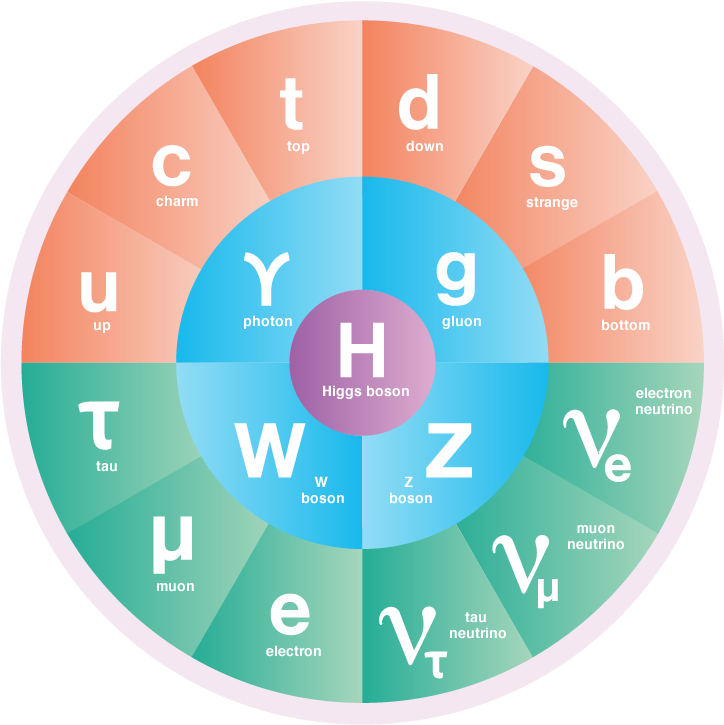
\includegraphics[width=\textwidth]{standard_model}
  \caption[][14.2em]{%
    The particles of the \gls{sm} are divided into subsets:
    quarks (orange), leptons (green), gauge bosons (blue) and the Higgos boson (violet).
    The up-like quarks ($u, c, t$) carry a charge of $\frac{2}{3}e$, while the down-like quarks' ($d, s, b$) charge is $-\frac{1}{3}e$.
    The three leptons on the left ($e, \mu, \tau$) have the charge $-e$, while the leptons on the right ($\nu_e, \nu_\mu, \nu_\tau$) are neutral.
    The gauge bosons are the mediators of electromagnetism ($\gamma$), weak interaction ($W^\pm, Z$) and strong interaction ($g$).
    The Higgs boson ($H$) is reponsible for the \gls{sm} fermions' mass.
    -- \copyright \href{http://www.symmetrymagazine.org/standard-model/}{symmetrymagazine.org}
  }
  \label{fig:standard_model}
\end{figure}

Mathematically speaking, the \gls{sm} is a gauge quantum field theory built upon internal symmetries of the unitary product group $SU(3) \times SU(2) \times U(1)$\marginnote{Unitary and special unitary groups of degree 1, 2 and 3}.

\subsection{The neutrino, from proposal to discovery}
Pauli proposed the existence of a neutral particle with almost no mass in 1930\cite{Brown:1978} to describe the continuous energy spectrum of $\beta$-decays without breaking the principle of energy conservation.
His spin $\frac{1}{2}$, neutral, light particle was practically undetectable, such that he considered his idea not to be in stage of publication.
Enrico Fermi developed a theory of $\beta$-decays based on Pauli's idea and introduced the name neutrino.
Supported by Fermi's theory, Pauli presented his idea in 1933.

The experimental proof of the existence of the neutrino was provided in 1956\marginnote{It took 23 years to proof the existence of neutrinos!} by Frederick Reines' and Clyde L. Cowan, Jr.'s.
The setup consisted of water tanks, liquid scintillator, photomultipliers, an efficient neutron absorber and some logic signal treatment.
Measuring a very characteristic signature of the inverse $\beta$-decay, led to a drastical reduction of the background\cite[-2.5em]{Reines:1995:NobelLecture}.
This made it possible to get significant results, placing the setup close to a nuclear reactor.

\begin{figure*}
  \centering
  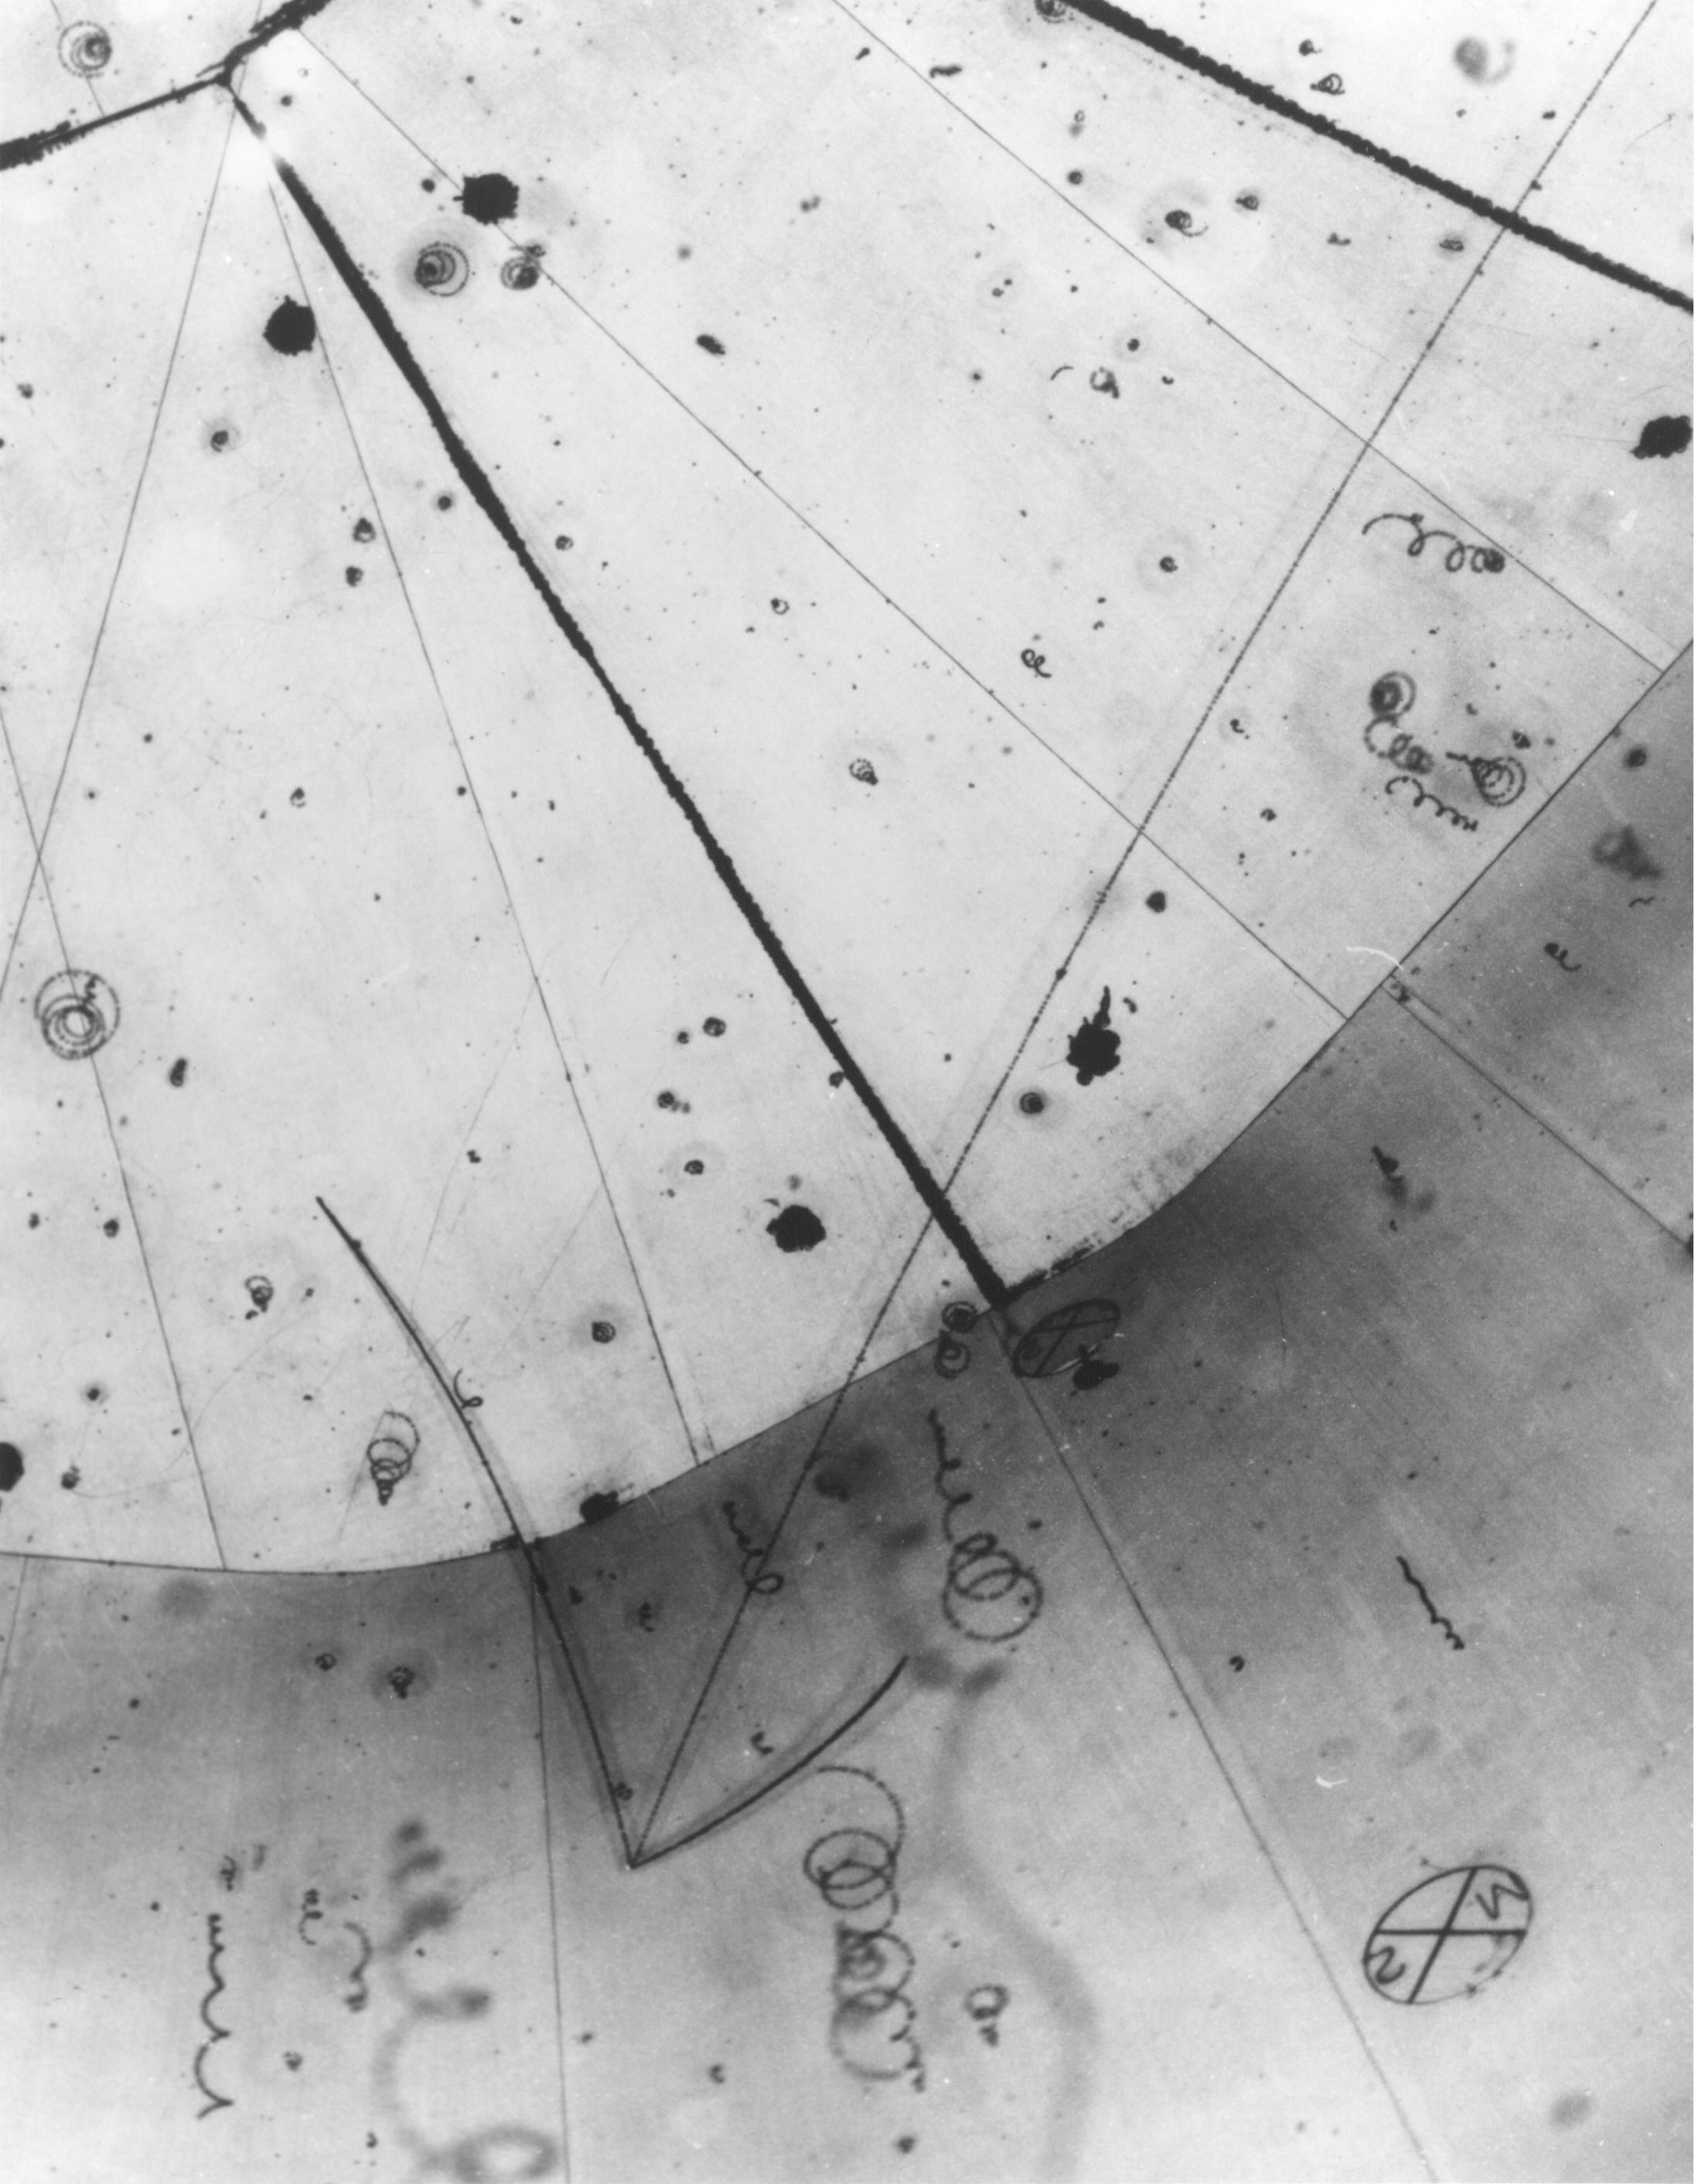
\includegraphics[width=.8\textwidth]{observation}
  \caption[][1em]{%
      World's first neutrino observation (Nov. 13th 1970)
      -- \copyright Argonne National Laboratory
  }
  \label{fig:observation}
\end{figure*}

The Argonne National Laboratory run the Zero Gradient Synchrotron from 1963 to 1979 and used a 12-foot hydrogen bubble chamber to record events from the accelerated particles and their byproducts.
Using this technology, it was possible to register the world's first neutrino observation on November 13th 1970, displayed in figure \ref{fig:observation}.
This event is the irrefutable proof of neutrino's existence.


\subsection{What are neutrino's properties?}
Despite the development of neutrino detectors over the last decades, some neutrino properties remain yet unknown.
Studying the properties of a particle is a good way to check our model's consistency or lead us to new, unknown physics.
This is a good reason to keep developing and running neutrino experiments.

\paragraph{Classification in the \gls{sm}} As proposed by Pauli, neutrinos are neutral particles of small mass with spin 1/2 and therefore fermions.
Neutrinos conserve leptonic number, making them part of the group of leptons.
Neutrinos come in 3 different flavors, and each flavor is associated to one of the heavier leptons: electron neutrino $\nu_e$, muon neutrino $\nu_\mu$ and tauon neutrino $\nu_\tau$.
The number of different light neutrino types was determined by studying Z-Boson production and decay\cite{Karlen:2004fj}.

\paragraph{Helicity} A handy way to group particles is by projecting a particle's spin along its direction of motion getting as a result its helicity.
Particles with a positive helicity are called right-handed, their counterpart is called left-handed.
So far there's no experimental evidence for right-handed neutrinos or left-handed antineutrinos\cite{1601.00627}\cite{Romero:2016str}.
The first hints for neutrino's helicity were given T.D. Lee and C.N. Yang.
They predicted in 1956 parity violation in weak interactions, by expressing the weak interaction as a chiral gauge interaction.
This was later shown by Chien-Shiung Wu in collaboration with the Low Temperature Group of the US National Bureau of Standards\cite{PhysRev.105.1413}.

\paragraph{Mass} Bruno Pontecorvo and Vladimir Gribov had an idea\marginnote{further developed by Ziro Maki, Masami Nakagawa and Shoichi Sakata}, which predicted that neutrinos undergo changes in flavor, called neutrino oscillations\cite{Bahcall:2004}.
Raymond Davis Jr. and John Bahcall's solar neutrino problem strongly indicated the existence of neutrino oscillations and Takaaki Kajita and Arthur B. McDonald confirmed this with their experiment.
Neutrino oscillations require neutrinos to have a non-zero mass and allow to study neutrino's relative mass.\marginnote{The \gls{sm} gives mass to fermions by the interaction with the Higgs field, which involves interactions with particles of both chiralities.
Since no right-handed neutrinos and left-handed antineutrinos were observed so far, it is not clear where the neutrino masses arise from.}
On the other hand the absolute mass of the three flavors of neutrinos remains unknown, such that different hierarchies are possible.
At the point of writing, two possible hierarchies are considered: the normal hierarchy and the inverted hierarchy.

\paragraph{Neutrino velocities} Due to their small mass, neutrinos generated in particle physics processes are expected to have velocities close to the one of light in vacuum\marginnote{So called hot matter}.
The velocity of neutrinos was measured in several experiments, confirming the theory's expectations\cite{Antonello:2012be}\cite{Adam:2011faa}.


\clearpage
\newpage

% - neutrino detectors
\section{Neutrino detection}

You cannot see a neutrino directly, but if it interacts with a particle in our detector, we might observe and identify the byproducts of the interaction.
A few techniques to determine neutrino fluxes and study neutrino's interactions with other particles have been developped.
This section lists some of these methods.

\subsection{Counting atoms}
When neutrinos interact with the neutrons in the atom, a lepton and a proton may be produced
\begin{equation*}
  \nu_e + n \to e^- + p^+,
\end{equation*}
changing the nuclear structure and chemical properties of the atom it interacted with.
If a tank is filled with pure homoatomic liquid and one is able to detect and count the resulting new atoms\marginnote{\emph{Chemists} know how to do this!} of the neutrino interactions, one can draw conclusions on the neutrinos and the neutrino flux.
If the production rate of neutrinos can be controlled, as it is the case with nuclear reactors, the results are even more evident.
And even though counting the number of atoms seems a difficult process, a number of experiments proove that it is feasable.\marginnote{Like the experiment run by John Bahcall and Raymond Davis Jr.}

\subsection{Observing chain interactions}
One could observe the subsequent reactions of the byproducts of the neutrino interaction\marginnote{This astute technique was used by Clyde Cowan and Frederick Reines to detect electron antineutrinos.} to conclude a neutrino interaction.
A clear signal raising from the background is needed for this cause.
For instance, the interaction of an electron antineutrino and a proton results in a neutron and a positron
\begin{equation*}
  \bar{\nu}_e + p^+ \to n + e^+.
\end{equation*}
The positron won't travel very far in matter until it annihilates with an electron, emitting two photons
\begin{equation*}
  e^+ + e^- \to \gamma + \gamma
\end{equation*}
with an energy of approximately half an MeV\marginnote{In a center of mass system, the photons' energy will be equivalent to the electron and positron's mass.} in opposite directions.
If the neutron is absorbed by the nucleus of some atom, the latter may react.
When cadmium absorbs a neutron, it'll go into a meta-stable state, which decays into its ground state by emmiting a gamma ray
\begin{equation*}
  n + \ce{^{108}Cd} \to \ce{^{109}Cd^*} \to \ce{^{109}Cd} + \gamma.
\end{equation*}
The time window from the neutrino interaction to the electron positron annihilation and the gamma emission of the nucleus is a determinant characteristic of the process.

\subsection{Cherenkov detectors} No particle faster than the speed of light in vacuum\marginnote{Physicists call these hypothetical particles \emph{tachions}.} was found so far.
But light's speed depends on the refractive index of the medium it is travelling through.
Therefore charged particles can travel through a suitable medium faster than light does, producing \emph{Cherenkov radiation}, a measurable cone of light.
This light can be read out to reconstruct the geometry of the cone and identify the particle which generated it.
Such cones are displayed in the illustrations of figure \ref{fig:super_kamiokande_events}.
Kamiokande, \gls{lsnd}, MiniBooNE and many other detectors used this technique.

\begin{figure*}
  \centering
  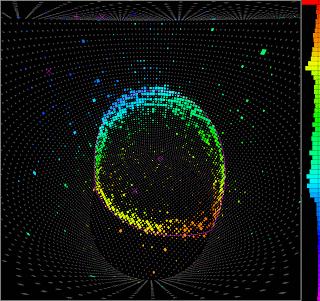
\includegraphics[width=.48\textwidth]{super_kamiokande/muon}
  \hspace*{1em}
  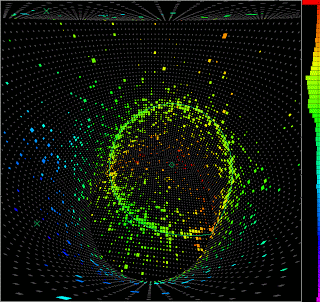
\includegraphics[width=.48\textwidth]{super_kamiokande/electron}
  \caption{%
    Images of events in Super Kamiokande.
    The illustration on the left shows a muon event, the one on the right an electron event.
    The muon's cone has a clean shape while the electron's cone is less evident.
    Electrons scatter more than muons, due to their lower mass, leading to a spread cone.
    The time scale of on the right displays the time window and energy deposit during the observation.
    -- \copyright Tomasz Barszczak - Super-Kamiokande Collaboration
  }
  \label{fig:super_kamiokande_events}
\end{figure*}

\subsection{Bubble \& cloud chambers} Another way to trace charged particles is by putting a fluid close to phase transition in their path.
When the charged particle interacts with the liquid, it produces heat, letting the fluid change its phase, such that bubbles will form.
Bubble chambers and cloud chambers use this effect to produce and image such traces.
The length, thickness and shape of the trace is determinant for the particle generating it.
To be able to reconstruct one event, several images from different angles are needed.
Figure \ref{fig:observation} is a good example of an interaction seen in such a detector.
\marginnote{Watch Professor Sumner Davis' \href{https://www.youtube.com/watch?v=HuIiKy_2F6g}{Advanced Laboratory on Bubble Chambers}}

\subsection{Photoemulsion films} Using a specially chosen chemical compound, which alters its state permanently after interacting with incident radiation, offers a further possibility to trace charged particles.
Photoemulsion films exploit this idea and lead to images like the one illustrated in figure \ref{fig:photoemulsion}.
The grains become visible after a development process, revealing the tracks left behind by the particles.
The OPERA experiment was able to proof the appearance of tauon neutrinos in a muon neutrino beam using this technique\cite{Ereditato2016116}.

\begin{figure}
  \centering
  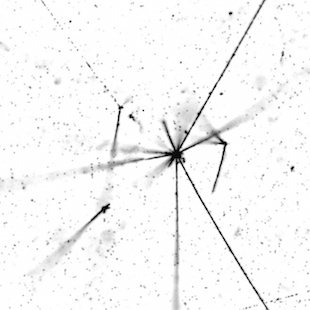
\includegraphics[width=.8\textwidth]{photoemulsion}
  \caption[][24.5em]{%
    Interaction of an anti-proton with a nucleon of an atom in a photo-emulsion film.
    The AEgIS experiment -- source of this event -- uses such emulsion films to measure the gravitational force on antihydrogen
    -- \copyright LHEP Universität Bern
  }
  \label{fig:photoemulsion}
\end{figure}

\subsection{Time projection chambers} In a medium the ionized atoms generated by the incident radiation recombine shortly after being ionized.
By applying an electric field, recombination can be supressed and the ionization electrons can be trapped, letting them drift through the fluid towards a charge collector.
The path can be reconstructed if the drift speed is constant and the time the particle was drifting is determined.
These kind of detectors are called \glspl{tpc}.
MicroBooNE, SBND and Icarus feature \gls{lartpc} in their apparati.
A few events as registered by the \glspl{lartpc} of MicroBooNE are displayed in figure \ref{fig:events_microboone}.

\begin{figure}
  \centering
  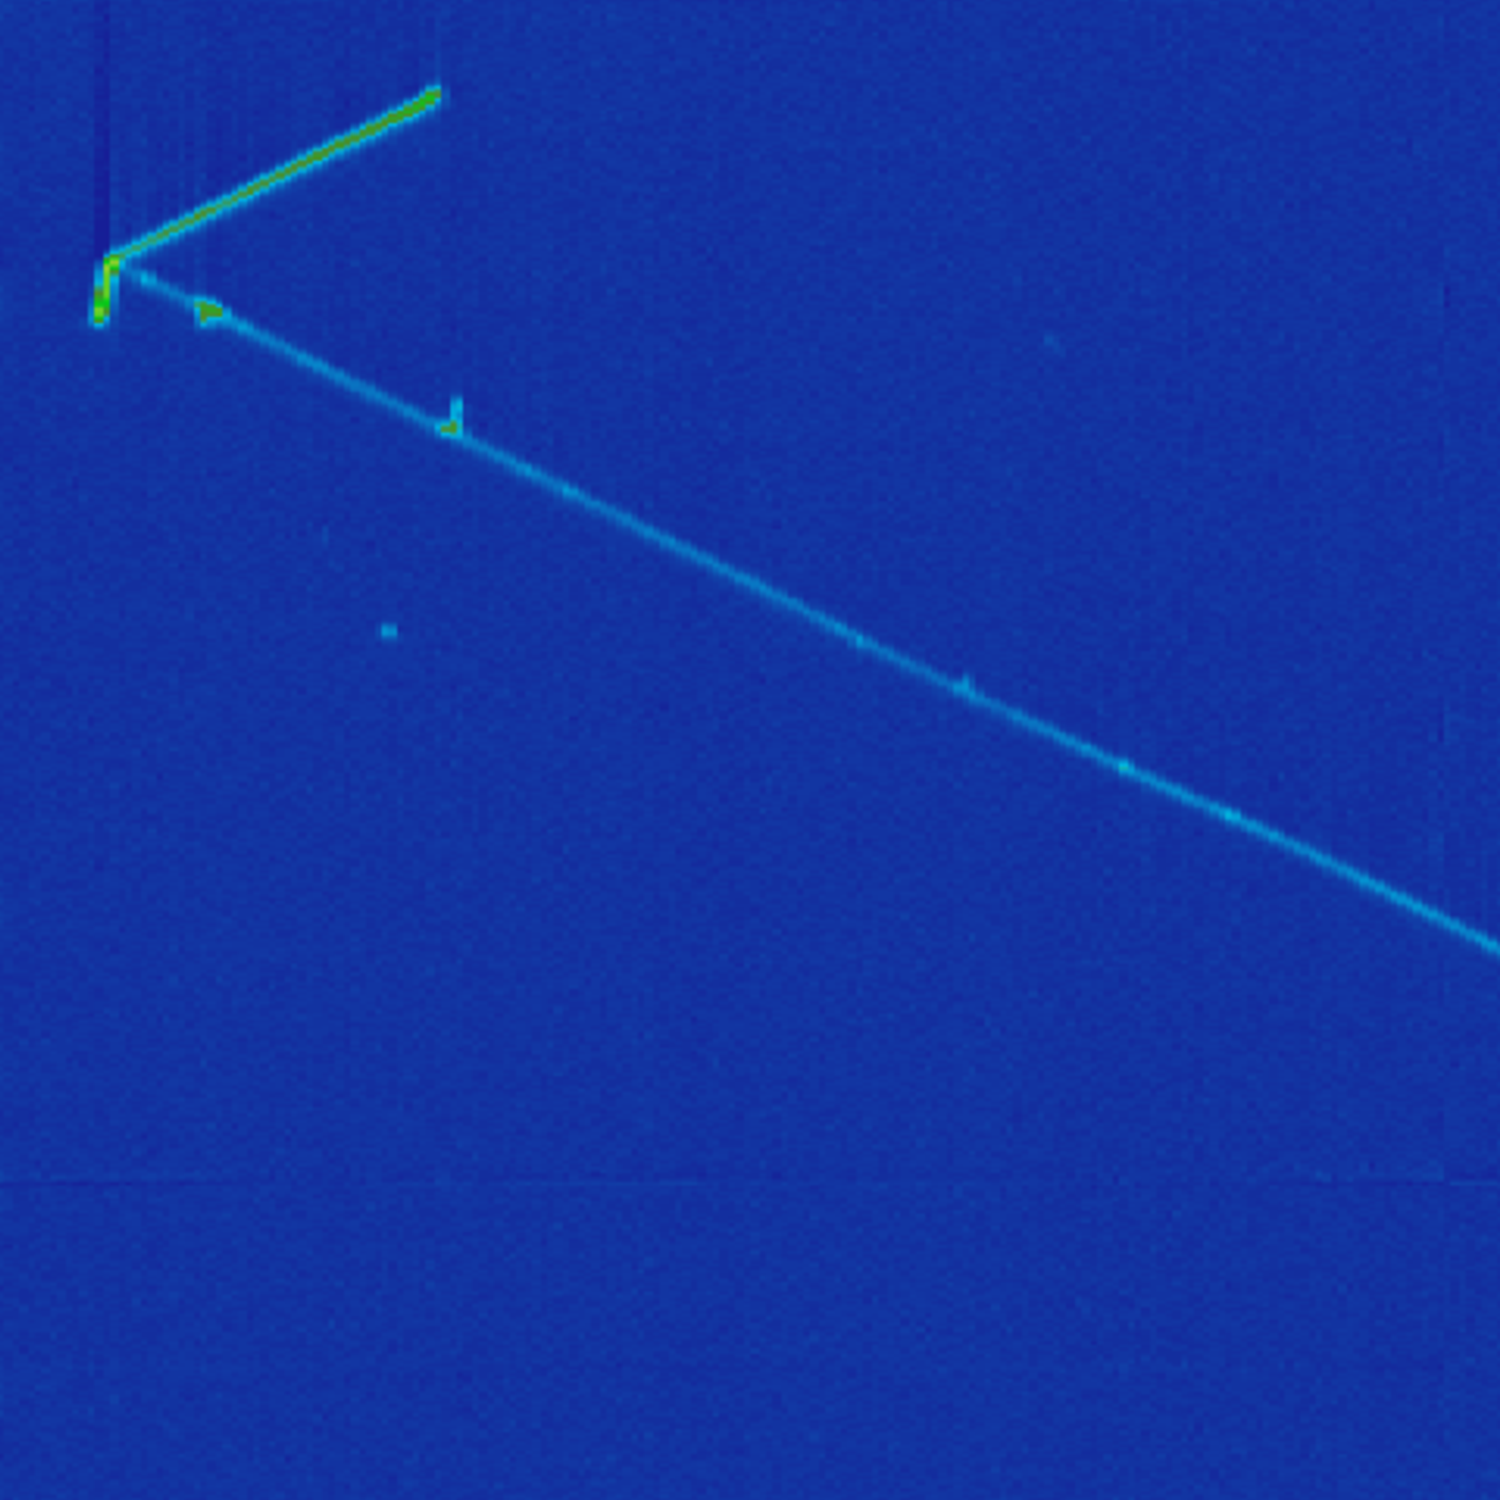
\includegraphics[width=.46\textwidth]{microboone_events/cut/ccqe}
  \hspace*{.5em}
  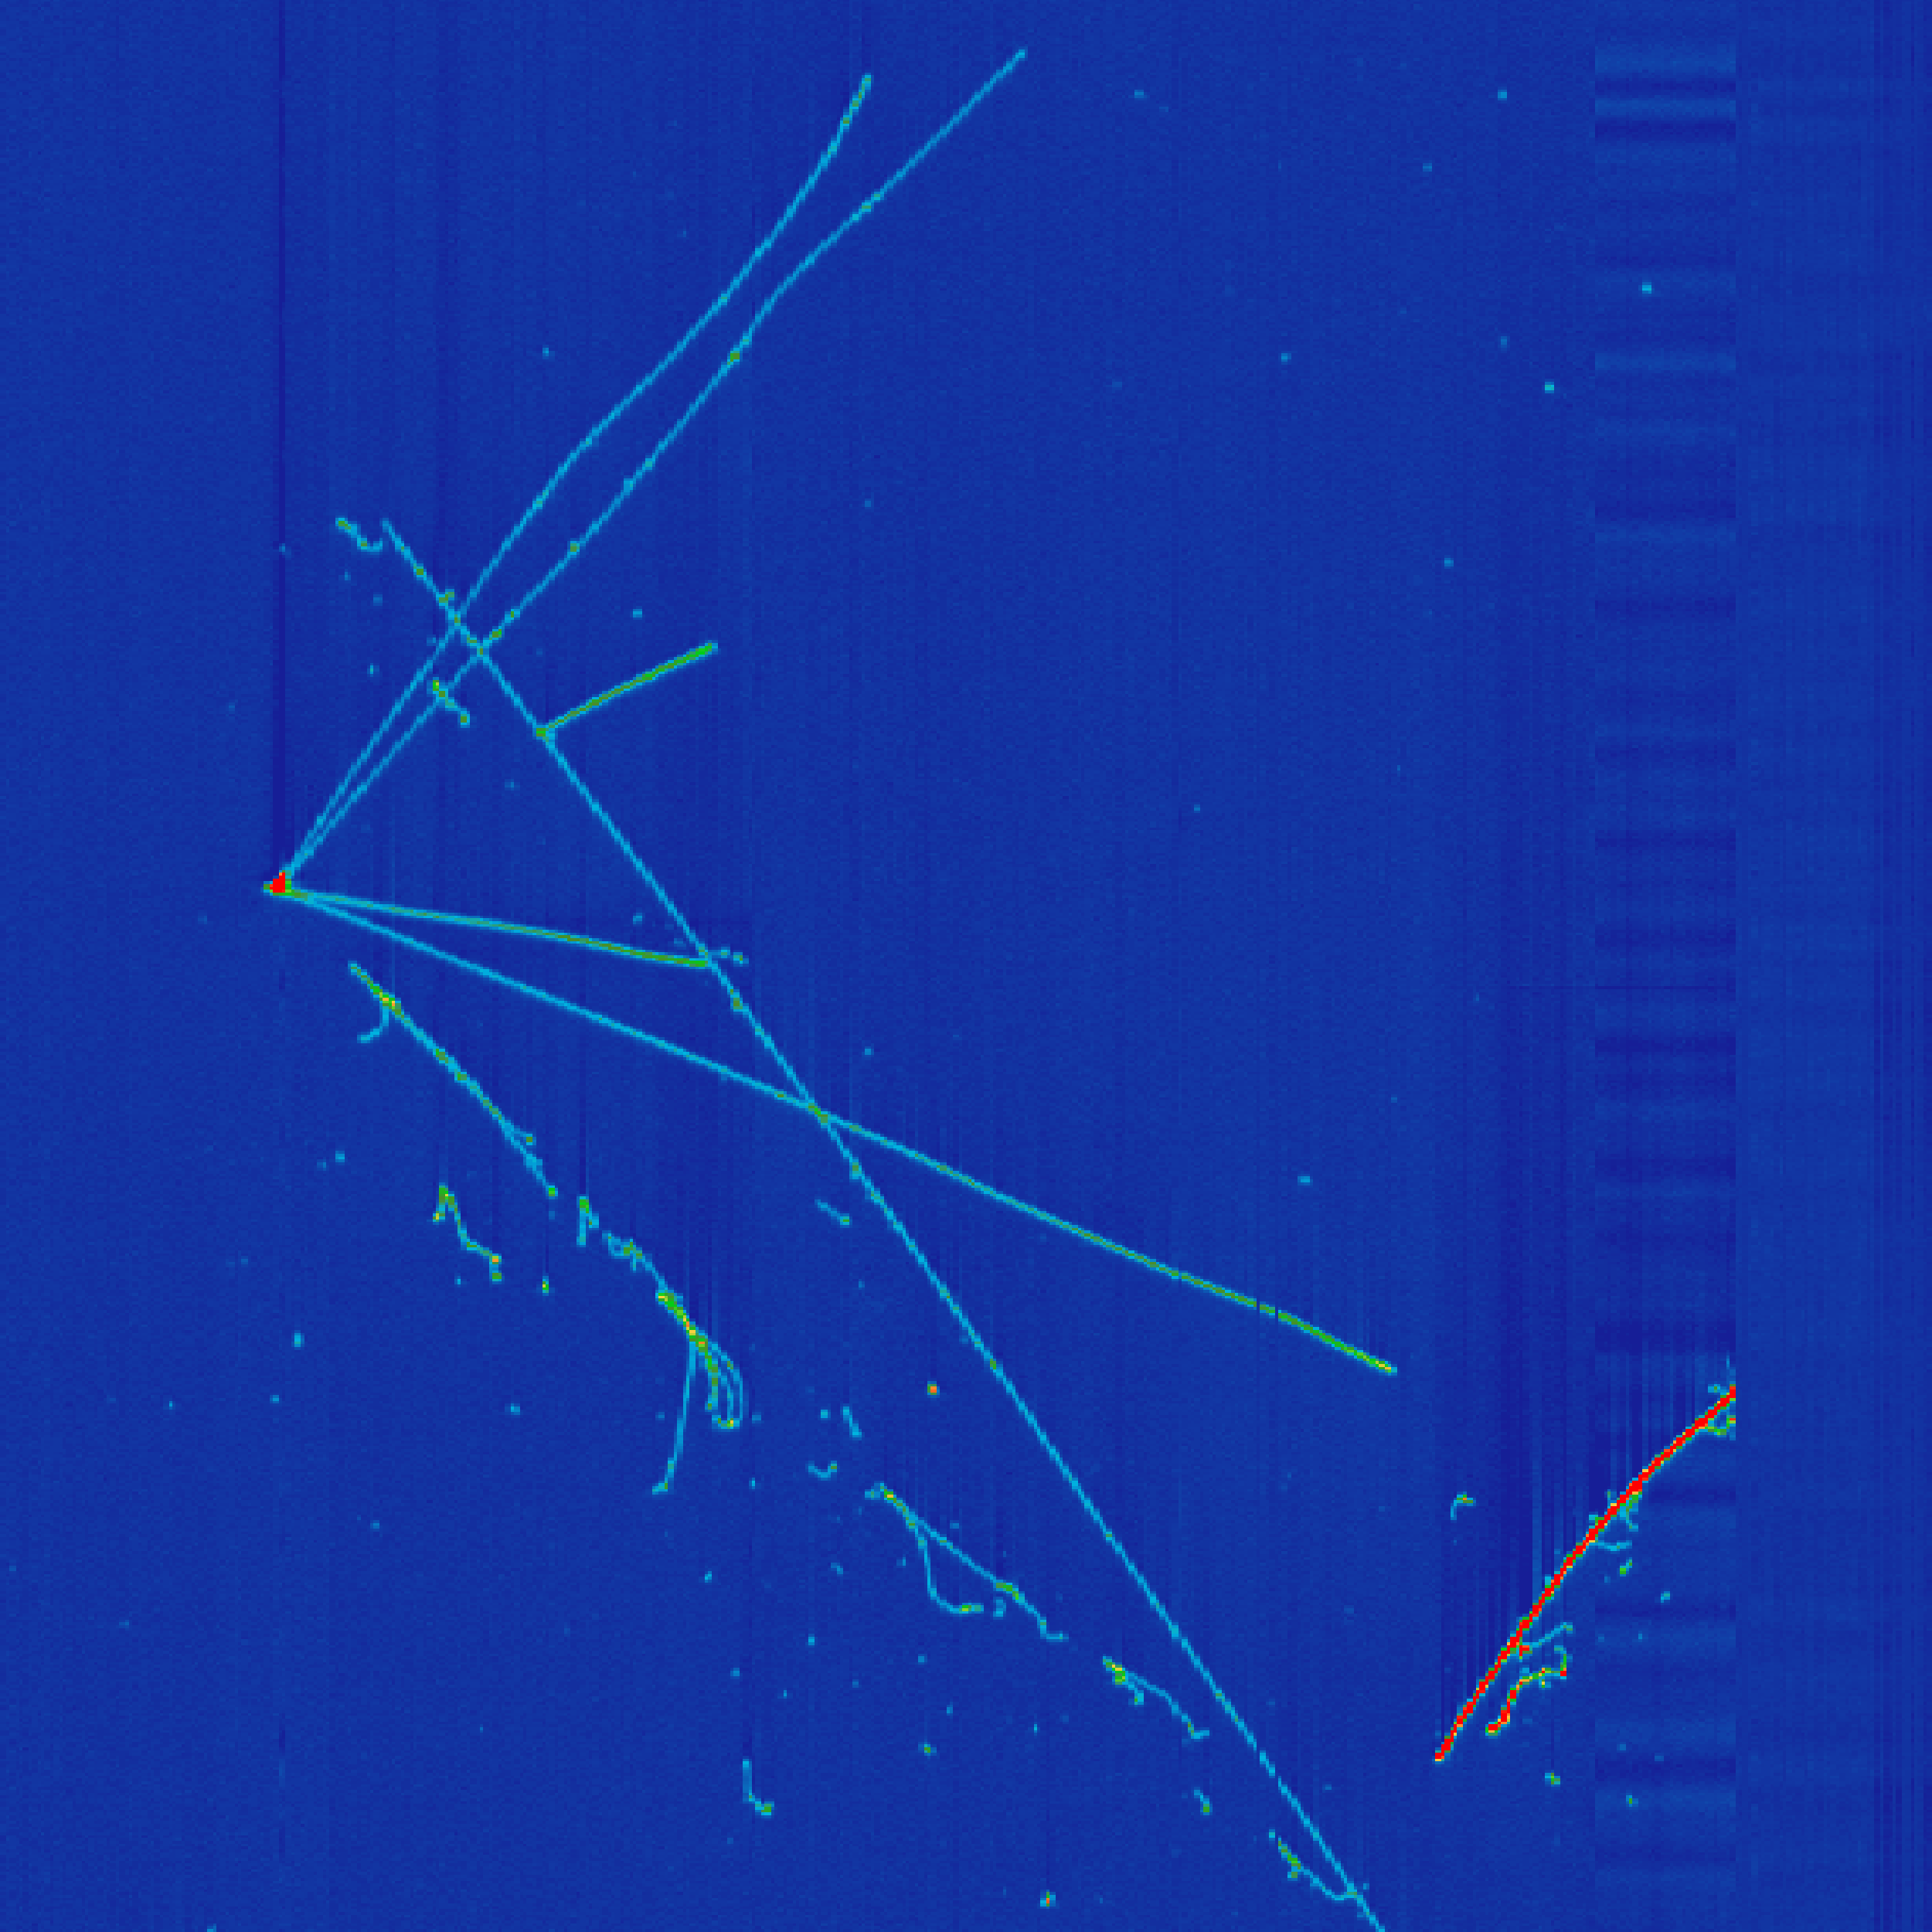
\includegraphics[width=.46\textwidth]{microboone_events/cut/dis}
  \caption{%
    The event on the left is a candidate of a quasi-elastic scattering event.
    The event on the right is probably a deep inelastic scattering event with a candidate of a cosmic ray.
    -- \copyright \href{http://www-microboone.fnal.gov/first-neutrinos/index.html}{fnal.gov}
  }
  \label{fig:events_microboone}
\end{figure}

\clearpage
\newpage

%% Theory
% - how do neutrinos interact
\section{Neutrino interactions}
Neutrinos are studied by observing their interactions.
It is therefore essential to know our model's neutrino interactions.
This section aims to list the known neutrino interacions using Feynman diagrams\marginnote{A handy tool to describe particle interactions! \href{https://www.youtube.com/watch?v=jNNXD7fuE5E}{Watch Feynman explaining their functionality in a lecture series at the University of Auckland in 1979.}}, classify events into common energy ranges using the energy-momentum transfer and list the elastic and quasi-elastic scattering interactions of neutrinos and anti-neutrinos.

\subsection{Currents of the weak interaction}
Ignoring gravitational interactions, neutrinos are assumed to interact only under weak interactions.
Consequently the involved mediators are the massive $W^\pm$- and the $Z$-boson\marginnote{Massive bosons: 80GeV and 91GeV. The high mass of the mediators is the reason for the short range of the weak interaction.}, the mediators for \glspl{cc} and \glspl{nc}.

\begin{figure}
  \centering
  \vspace{1em}
  \begin{fmffile}{nc}
    \begin{fmfgraph*}(135,75)
      \fmfleft{i1,i2}
      \fmfright{o1,o2}
      \fmf{fermion}{i1,v1,o1}
      \fmf{phantom}{i2,v2,o2}
      \fmf{photon}{v1,v2}
      \fmflabel{$\nu$}{i1}
      \fmflabel{$\nu$}{o1}
      \fmflabel{$Z$}{v2}
    \end{fmfgraph*}
    \hspace*{2em}
    \begin{fmfgraph*}(135,75)
      \fmfleft{i1,i2}
      \fmfright{o1,o2}
      \fmf{fermion}{o1,v1,i1}
      \fmf{phantom}{i2,v2,o2}
      \fmf{photon}{v1,v2}
      \fmflabel{$\bar{\nu}$}{i1}
      \fmflabel{$\bar{\nu}$}{o1}
      \fmflabel{$Z$}{v2}
    \end{fmfgraph*}
  \end{fmffile}

  \vspace*{2em}

  \begin{fmffile}{cc}
    \begin{fmfgraph*}(135,75)
      \fmfleft{i1,i2}
      \fmfright{o1,o2}
      \fmf{fermion}{i1,v1,o1}
      \fmf{phantom}{i2,v2,o2}
      \fmf{photon}{v1,v2}
      \fmflabel{$\nu_l$}{i1}
      \fmflabel{$l$}{o1}
      \fmflabel{$W^+$}{v2}
    \end{fmfgraph*}
    \hspace*{2em}
    \begin{fmfgraph*}(135,75)
      \fmfleft{i1,i2}
      \fmfright{o1,o2}
      \fmf{fermion}{o1,v1,i1}
      \fmf{phantom}{i2,v2,o2}
      \fmf{photon}{v1,v2}
      \fmflabel{$\bar{\nu}_l$}{i1}
      \fmflabel{$\bar{l}$}{o1}
      \fmflabel{$W^-$}{v2}
    \end{fmfgraph*}
  \end{fmffile}
  \caption{%
    Feynman diagrams of (ftltbr) neutrino and anti-neutrino interacting with neutral and charged currents.
  }
  \label{fig:currents}
  \vspace{1em}
\end{figure}

For interactions mediated by a \gls{nc} the neutrino remains a neutrino and the anti-neutrino remains an anti-neutrino.
When a neutrino interacts with another particle mediated by a \gls{cc} the resulting particle is the neutrino's associated lepton.
Anti-neutrinos consequently become their associated anti-lepton.
Since the lepton and anti-lepton's charge differ, the currents -- and therefore the mediators -- need to differ as well.\marginnote{Due to conservation of charge.}
Figure \ref{fig:currents} displays the Feynman diagrams of these two interactions.

\subsection{Energy-momentum transfer and event classification}

The interactions can be classified using the energy-momentum transfer between the interacting particles.
Assuming we know the initial and final four-momenta of an interacting particle $p_i^\mu = (E_i, \vec{p}_i)$ and $p_f^\mu = (E_f, \vec{p}_f)$, then the momentum energy transfer is given by
\begin{equation*}
  q = p_i^\mu - p_f^\mu = (\Delta E, \Delta \vec{p}).
\end{equation*}

\begin{figure}
  \centering
  \vspace{1em}
  \begin{tikzpicture}
    \draw[->]         (-3,2) -- node (a) [label={above:$\vec{p}_i$}] {} (0,0);
    \draw[->]         (0,0)  -- node (b) [label={above:$\vec{p}_f$}] {} (2,1);
    \draw[->, dashed] (0,0)  -- node (c) [label={left:$\vec{q}$}] {} (1,-3);
  \end{tikzpicture}
  \hspace*{4em}
  \begin{tikzpicture}
    \draw[->]         (-3,3) -- node (a) [label={above:$\vec{p}_i$}] {} (0,1);
    \draw[->]         (0,1)  -- node (b) [label={below:$-\vec{p}_f$}] {} (-2,0);
    \draw[->, dashed] (-3,3)  -- node (c) [label={left:$\vec{q}$}] {} (-2,0);
  \end{tikzpicture}
  \vspace{1em}
  \caption{%
    Illustration of the momentum transfer.
    $\vec{p}_i$ and $\vec{p}_f$ indicate the initial and final momenta.
    The image on the left shows the interaction of a classical particle transfering the momentum $\vec{q}$.
    If the momenta are rearranged like in the image on the right, it is obvious that $\vec{q}$ is given by $\vec{p}_i - \vec{p}_f$.
  }
  \label{fig:q}
\end{figure}

Given a flat Minkowski-space, the square of the norm of $q$ is given by
\begin{equation*}
  |q|^2 = (\Delta \vec{p})^2 - (\Delta E)^2,
\end{equation*}
where $\Delta E$ is the total transferred energy and $\Delta \vec{p}$ the total transferred momentum.
We can define how massive an event is\marginnote{See the analogy to $m^2 = E^2 - p^2$?}
\begin{align*}
  Q^2 &= (\Delta E)^2 - (\Delta \vec{p})^2 \\
      &= -q^2,
\end{align*}
and use this factor $Q^2$ to classify neutrino interaction events into:\\
\begin{tabular}{ l c }
  Elastic \& quasi-elastic scattering  & $Q^2 < 1 \text{GeV}^2$ \\
  Resonant scattering                  & $Q^2 \approx 1 \text{GeV}^2$ \\
  Deep inelastic scattering            & $Q^2 > 1 \text{GeV}^2$ \\
\end{tabular}

\subsection{Elastic \& quasi-elastic scattering} 
Interactions of $Q^2$ below 1GeV$^2$ are called elastic scattering events if they were mediated by the \gls{nc}.
Low energy scattering events mediated by \gls{cc} do not conserve kinetic energy, since part of it is needed to come up for the mass difference of the neutrino and its associated charged lepton.
For this reason these events are called quasi-elastic.
The terms \gls{ccqe} and \gls{nce} are commonly used to referr to these two classes of events.

If we list all possible interactions of neutrinos and anti-neutrinos with matter and anti-matter, we can see, that there's a clear symmetry in the case of the \gls{nce} -- see figure \ref{fig:elastic}.
The diagram for interactions of neutrinos with matter is equivalent to the diagram for the interactions of anti-neutrinos with anti-matter.
The same occurrs for interacions of neutrinos with anti-matter and anti-neutrinos with matter.

\begin{figure}
  \centering
  \vspace{1em}
  \begin{fmffile}{elastic}
    \begin{fmfgraph*}(135,75)
      \fmfleft{i1,i2}
      \fmfright{o1,o2}
      \fmf{fermion}{i1,v1,o1}
      \fmf{fermion}{i2,v2,o2}
      \fmf{photon,label=$Z$}{v1,v2}
      \fmflabel{$\nu_l$}{i1}
      \fmflabel{$q, l$}{i2}
      \fmflabel{$\nu_l$}{o1}
      \fmflabel{$q, l$}{o2}
    \end{fmfgraph*}
    \hspace*{2em}
    \begin{fmfgraph*}(135,75)
      \fmfleft{i1,i2}
      \fmfright{o1,o2}
      \fmf{fermion}{i1,v1,o1}
      \fmf{fermion}{o2,v2,i2}
      \fmf{photon,label=$Z$}{v1,v2}
      \fmflabel{$\nu_l$}{i1}
      \fmflabel{$\bar{q}, \bar{l}$}{i2}
      \fmflabel{$\nu_l$}{o1}
      \fmflabel{$\bar{q}, \bar{l}$}{o2}
    \end{fmfgraph*}

    \vspace*{4em}

    \begin{fmfgraph*}(135,75)
      \fmfleft{i1,i2}
      \fmfright{o1,o2}
      \fmf{fermion}{o1,v1,i1}
      \fmf{fermion}{i2,v2,o2}
      \fmf{photon,label=$Z$}{v1,v2}
      \fmflabel{$\bar{\nu}_l$}{i1}
      \fmflabel{$q, l$}{i2}
      \fmflabel{$\bar{\nu}_l$}{o1}
      \fmflabel{$q, l$}{o2}
    \end{fmfgraph*}
    \hspace*{2em}
    \begin{fmfgraph*}(135,75)
      \fmfleft{i1,i2}
      \fmfright{o1,o2}
      \fmf{fermion}{o1,v1,i1}
      \fmf{fermion}{o2,v2,i2}
      \fmf{photon,label=$Z$}{v1,v2}
      \fmflabel{$\bar{\nu}_l$}{i1}
      \fmflabel{$\bar{q}, \bar{l}$}{i2}
      \fmflabel{$\bar{\nu}_l$}{o1}
      \fmflabel{$\bar{q}, \bar{l}$}{o2}
    \end{fmfgraph*}
  \end{fmffile}
  \caption{%
    First order neutrino elastic scattering Feynman diagrams.
    $q$ stands for a quark of any flavor in a baryon, since quarks are not found free in nature.
    The diagram on the top left is equivalent to the diagram on the bottom right.
    The diagrams on the top right and the bottom left are equivalent as well.
  }
  \label{fig:elastic}
  \vspace{1em}
\end{figure}

\Gls{ccqe} lack such a symmetry, i.e. none of the four diagrams is equivalent -- see figure \ref{fig:quasielastic}.
Similar diagrams are found by changing the involved particles and mediators by their anti-particles and viceversa.

\begin{figure}
  \centering
  \vspace{1em}
  \begin{fmffile}{quasi}
    \begin{fmfgraph*}(135,75)
      \fmfleft{i1,i2}
      \fmfright{o1,o2}
      \fmf{fermion}{i1,v1,o1}
      \fmf{fermion}{i2,v2,o2}
      \fmf{photon,label=$W$}{v1,v2}
      \fmflabel{$\nu_l$}{i1}
      \fmflabel{$d, l$}{i2}
      \fmflabel{$l$}{o1}
      \fmflabel{$u, \nu$}{o2}
    \end{fmfgraph*}
    \hspace*{2em}
    \begin{fmfgraph*}(135,75)
      \fmfleft{i1,i2}
      \fmfright{o1,o2}
      \fmf{fermion}{i1,v1,o1}
      \fmf{fermion}{o2,v2,i2}
      \fmf{photon,label=$W$}{v1,v2}
      \fmflabel{$\nu_l$}{i1}
      \fmflabel{$\bar{u}$}{i2}
      \fmflabel{$l$}{o1}
      \fmflabel{$\bar{d}$}{o2}
    \end{fmfgraph*}

    \vspace*{4em}

    \begin{fmfgraph*}(135,75)
      \fmfleft{i1,i2}
      \fmfright{o1,o2}
      \fmf{fermion}{o1,v1,i1}
      \fmf{fermion}{i2,v2,o2}
      \fmf{photon,label=$W$}{v1,v2}
      \fmflabel{$\bar{\nu}_l$}{i1}
      \fmflabel{$u$}{i2}
      \fmflabel{$\bar{l}$}{o1}
      \fmflabel{$d$}{o2}
    \end{fmfgraph*}
    \hspace*{2em}
    \begin{fmfgraph*}(135,75)
      \fmfleft{i1,i2}
      \fmfright{o1,o2}
      \fmf{fermion}{o1,v1,i1}
      \fmf{fermion}{o2,v2,i2}
      \fmf{photon,label=$W$}{v1,v2}
      \fmflabel{$\bar{\nu}_l$}{i1}
      \fmflabel{$\bar{d}$, $\bar{l}$}{i2}
      \fmflabel{$\bar{l}$}{o1}
      \fmflabel{$\bar{u}$, $\bar{\nu}_l$}{o2}
    \end{fmfgraph*}
  \end{fmffile}
  \caption{%
    First order Feynman diagrams for quasielastic scattering.
    $u$ and $d$ stand for up-like and down-like quarks in a baryon.
    No equivalence can be found in these diagrams.
  }
  \label{fig:quasielastic}
  \vspace{1em}
\end{figure}


\clearpage
\newpage

% The short baseline neutrino detector
\section{Neutrino sources}

Neutrinos have a very small cross-section and interact very rarely\marginnote{\ldots and matter is virtually transparent for them}.
Many neutrinos emerge from natural and non natural sources adding an important signal background to any observation.
It is important to quantify the background's value of any source whose neutrinos may interact in our detector and bias our observations.
This section covers known natural and human induced neutrino sources.

\subsection{Natural sources}

\paragraph{Geoneutrinos} are neutrino emitted in a $\beta$-decay of a radionuclide naturally occurring in the Earth.
Most geoneutrinos are electron antineutrinos and originate from $\beta^-$-decay-branches of $\ce{^{40}K}$, $\ce{^{232}Th}$ and $\ce{^{238}U}$.
Referr to Geo-neutrinos\cite{2013PrPNP:73:1B} for a detailed review and analysis of the results from the KamLAND and Borexino data.

\paragraph{Atmospheric neutrinos} result from the interaction of cosmic rays with an atomic nucleus in the Earth's atmosphere.
These interactions generate showers of unstable particles -- mostly pions ($\pi$) -- whose decay involves the production of neutrinos.
For more information on cosmic rays refer to section on background detection and mitigation..
The atmospheric neutrino flux is studied using the data of the IceCube experiment\cite[-6em]{Aartsen:2016xlq} and Super-Kamiokande\cite[-1em]{Richard:2015aua}.

\paragraph{Solar neutrinos} The greatest neutrino background contribution is made by the sun.
The main solar neutrino radiation\marginnote{86\% of the solar neutrinos are produced by: $p + p \to d + e^+ + \nu_e$} comes from the proton-proton reaction, which is one of the known fusion reactions by which stars convert hydrogen to helium.
Important contributions are made by the reactions of beryllium and boron\marginnote[-.5em]{%
\setlength{\parindent}{0pt}%
$\ce{^7Be} + e^- \to \ce{^7Li} + \nu_e$, \\
$\ce{^8B} \to \ce{^8Be^*} + e^+ + \nu_e$}.
Solar neutrinos are best reviewed with the data of the Sudbury Neutrino Observatory\cite{Bellerive:2016byv}.

\subsection{Other sources}

\paragraph{Reactor neutrinos} Neutrinos emerging from interactions in nuclear reactors\marginnote{Nuclear scientific reactors, powerplants, nuclear submarines, etc.} are called reactor neutrinos.
The emission spectrum depends strongly on the type of nuclear reactions produced in the reactor\marginnote{So studying a reactor's neutrino spectrum allow to study nuclear power plants.}.

\paragraph{Neutrino beams} When particles in rest decay by a two body decay, the energy and momenta of the resulting particles are known exactly.
It is well known that the lightest charged mesons ($\pi^\pm$) decay into muons and their associated neutrinos, therefore the previous effect can be taken in advantage to build a neutrino beam out of decaying charged pions.


\clearpage
\newpage

% The short baseline neutrino detector
\section{Neutrino oscillations and anomalies in the observations}

Neutrino oscillations have been observed by numerous experiments, yet there's a discrepance in the results of the different experiments.
It is important to know how neutrino oscillations are modeled and the possible effects that alter our expected observations.
This section includes simple oscilation models, matter effects and results from the neutrino oscillation experiments \gls{lsnd} and MiniBooNE.

\subsection{Neutrino oscillation models}

Neutrino oscillations are a consequence of flavour neutrino mixing\marginnote{\ldots or lepton mixing} in vacuum\cite{Agashe:2014kda}.
This can be modeled using a linear combination of the fields of the massive neutrinos $\nu_m$ for the flavor neutrino field $\nu_f$ in the charged current weak interaction
\begin{equation*}
  \nu_f = \sum_m U_{fm}\nu_m,
\end{equation*}
where $f \in \{e, \mu, \tau\}$ is the index for the flavor eigentstate and $m \in \{1, 2, 3\}$ is the index for the mass eigenstate.

$U_{fm}$ is an unitary matrix generally called \emph{mixing} matrix\marginnote{\ldots but also known as the Pontecorvo-Maki-Nakagawa-Sakata (PMNS) mixing matrix}.
The parametrization of this unitary matrix depends on the number of neutrino flavors and their characterization into \emph{Majorana} or \emph{Dirac} particles\marginnote{Whilst Majorana particles are their own anti-particles, particle and anti-particle differ when dealing with Dirac particles.}.
Assuming there are $n$ neutrino flavors and $n$ massive neutrinos, the mixing matrix $U$ can be parametrized by $\frac{n(n-1)}{2}$ Euler angles (see figure \ref{fig:euler_angles}) and $\frac{n(n+1)}{2}$ phases in the case of Majorana neutrinos or $\frac{(n-1)(n-2)}{2}$ phases if neutrinos are Dirac particles\cite{Xing:2013woa}.

In the following 3 types of flavor field and mass field eigenstates are assumed.
We impose furthermore, that none of the eigenstates is identical to another
\begin{align*}
  \braket{\nu_{l'}}{\nu_l}             = \delta_{l'l}, \quad
  \braket{\bar{\nu}_{l'}}{\bar{\nu}_l} = \delta_{l'l}, \quad
  \braket{\bar{\nu}_{l'}}{\nu_l}       = 0,
\end{align*}
where $l \in \{e, \mu, \tau\}$ or $l \in \{1, 2, 3\}$.

In the case of Dirac massive neutrinos the representation of $U$ is given the three angles $\theta_{12}, \theta_{13}, \theta_{23}$ and just one \gls{cp} violation phase $\delta$
\begin{marginfigure}
  \centering
  \vspace*{1em}
  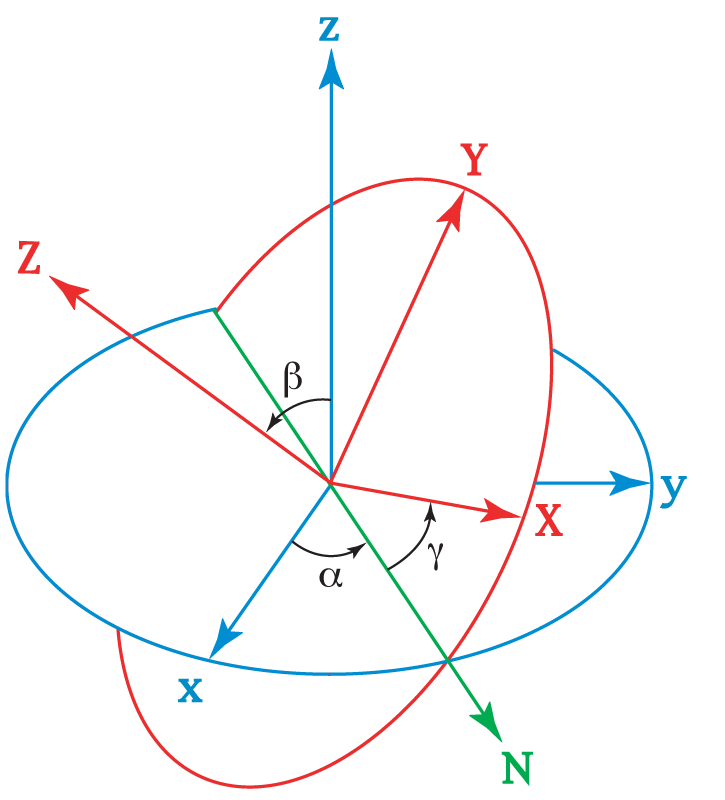
\includegraphics[width=\textwidth]{eulerangles}
  \caption{Illustration of the Euler angles between two rotated 3 dimensional reference frames.
  -- \copyright \href{https://commons.wikimedia.org/wiki/File:Euler.png}{wikimedia.org}}
  \label{fig:euler_angles}
\end{marginfigure}
\begin{align*}
  U_D &= \begin{bmatrix}
      U_{e 1} & U_{e 2} & U_{e 3} \\
      U_{\mu 1} & U_{\mu 2} & U_{\mu 3} \\
      U_{\tau 1} & U_{\tau 2} & U_{\tau 3}
    \end{bmatrix} \\
    &= \begin{bmatrix}
      1 & 0 & 0 \\
      0 & c_{23} & s_{23} \\
      0 & -s_{23} & c_{23}
    \end{bmatrix} \begin{bmatrix}
      c_{13} & 0 & s_{13}e^{-i\delta} \\
      0 & 1 & 0 \\
      -s_{13}e^{i\delta} & 0 & c_{13}
    \end{bmatrix} \begin{bmatrix}
      c_{12} & s_{12} & 0 \\
      -s_{12} & c_{12} & 0 \\
      0 & 0 & 1
    \end{bmatrix} \\
    &= \begin{bmatrix}
      c_{12}c_{13} & s_{12}c_{13} & s_{13}e^{-i\delta} \\
      -s_{12}c_{23} - c_{12}s_{23}s_{13}e^{i\delta} & c_{12}c_{23} - s_{12}s_{23}s_{13}e^{i\delta} & s_{23}c_{13} \\
      s_{12}s_{23} - c_{12}c_{23}s_{13}e^{i\delta} & -c_{12}s_{23} - s_{12}c_{23}s_{13}e^{i\delta} & c_{23}c_{13}
    \end{bmatrix},
\end{align*}
where $c_{ij} = \cos(\theta_{ij})$ and $s_{ij} = \sin(\theta_{ij})$.

If neutrinos are Majorana particles, two more \gls{cp} phases are needed.
These two phases can be can be taken into account by multiplying $U_D$ with a diagonal matrix $P$ containing the additional Majorana \gls{cp} violation phases $\rho$ and $\sigma$
\begin{align*}
  U_M &= U_D P \\
    &= \begin{bmatrix}
      U_{e 1} & U_{e 2} & U_{e 3} \\
      U_{\mu 1} & U_{\mu 2} & U_{\mu 3} \\
      U_{\tau 1} & U_{\tau 2} & U_{\tau 3}
    \end{bmatrix} \begin{bmatrix}
      e^{i\rho} & 0 & 0 \\
      0 & e^{i\sigma} & 0 \\
      0 & 0 & 1
    \end{bmatrix}.
\end{align*}

\subsection{Two flavor oscillation probabilities in vacuum}
The neutrino oscillation probability's complexity is reduced if assumed only two flavor eigenstates $(\nu_e, \nu_\mu)$ and two mass eigenstates $(\nu_1, \nu_2)$\marginnote{With only 2 Dirac neutrinos, the number of euler angles reduce to 1 and no phases appear.}.
In that case the mixing matrix reduces to
\begin{align*}
  U &= \begin{bmatrix}
      U_{e 1} & U_{e 2} \\
      U_{\mu 1} & U_{\mu 2}
    \end{bmatrix} \\
    &= \begin{bmatrix}
      \cos(\theta) & \sin(\theta) \\
      -\sin(\theta) & \cos(\theta)
    \end{bmatrix},
\end{align*}
where $\theta$ is the euler angle.
Consequently the flavor neutrinos can be written down in the form
\begin{align*}
  \ket{\nu_e}   &= \cos(\theta)\ket{\nu_1}  + \sin(\theta)\ket{\nu_2}, \\
  \ket{\nu_\mu} &= -\sin(\theta)\ket{\nu_1} + \cos(\theta)\ket{\nu_2}.
\end{align*}

Since the solutions of a plane wave can be used to describe the propagation of the mass eigenstates, we can state
\begin{equation*}
  \ket{\nu_m(t)} = e^{-i(E_m t - p_m x)}\ket{\nu_m(0)},
\end{equation*}
where $E_m$ and $p_m$ are the energy and momentum of the $m$th eigenstate\marginnote{The momentum of the particle is simplified to one dimension}.
The probability to find an electron neutrino in a beam of muon neutrinos is given by
\marginnote[1em]{%
  \setlength{\parindent}{5pt}%
  Used identities: \\
  $\braket{\nu_{l'}}{\nu_l} = \delta_{l'l}$ \\
  $\Delta E = E_1 - E_2$ \\
  $p_1 = p_2$ \\
  $\sin^2(\varphi)\cos^2(\varphi) = \frac{1}{4}\sin^2(2\varphi)$ \\
  $e^{i\varphi} = \cos(\varphi) + i \sin(\varphi)$ \\
  $\cos(\varphi) = \cos(-\varphi)$ \\
  $\sin(\varphi) = - \sin(-\varphi)$ \\
  $1 - \cos(2\varphi) = 2 \sin^2(\varphi)$
}
\begin{align*}
  P_{\nu_\mu \to \nu_e} &= |\braket{\nu_e(t)}{\nu_\mu}|^2 \\
  &= |\sin(\theta)\cos(\theta)(e^{-i(E_1t - p_1x)} - e^{-i(E_2t - p_2x)})|^2 \\
  &= \sin^2(\theta)\cos^2(\theta)\left(2 - e^{-i\Delta E t} - e^{i\Delta E t} \right) \\
  &= \frac{1}{2}\sin^2(2\theta)\left(1 + \cos(\Delta E t) \right) \\
  &= \sin^2(2\theta)\sin^2(\frac{\Delta E t}{2}).
\end{align*}

Since neutrinos' mass is very small in comparison to their momentum, we can approximate their energy by the Taylor expansion around $p_i$ and set $p_i \approx E_i \approx E$ getting
\begin{align*}
  E_i &= \sqrt{p_i^2 + m_i^2} \\
      &\approx p_i + \frac{m_i^2}{2E_i} \\
      &\approx E + \frac{m_i^2}{2E},
\end{align*}
to find
\marginnote[5em]{It's $\Delta(m^2)$ not $(\Delta m)^2$!}
\begin{align*}
  \Delta E &= \frac{m_1^2 - m_2^2}{2E} \\
           &= \frac{\Delta m^2}{2E}.
\end{align*}

Setting $t \approx \frac{L}{c} = L$ -- since neutrinos are always ultrarelativistic -- leads to the well known formula for two flavor neutrino oscillations
\begin{align*}
  P_{\nu_\mu \to \nu_e}(L) = \sin^2(2\theta) \sin^2(\Delta m^2 \frac{L}{4 E})
\end{align*}

Knowing the energy $E$ of the muon neutrino flux and the distance $L$ between the source of the muon neutrino flux and the detector the angle $\theta$ can be determined.

\subsection{Matter effects}
The occurring neutrino interactions depend on the type of matter and the neutrino flavor.
Since condensed matter is composed mainly of netrons, protons and electrons the possible interactions for muon and tauon neutrinos $\nu_\mu$, $\nu_\tau$ reduce to the interactions with hadronic matter, while electron neutrinos $\nu_e$ interact with the electrons as well.
Hence matter affects the passage of neutrinos of different flavors differently.\marginnote{\ldots the Michejew-Smirnow-Wolfenstein effect}
This can be elucidated by taking a look at the Feynman diagrams for the neutrino interactions with matter.

\begin{figure}
  \centering
  \vspace{2em}
  \begin{fmffile}{matter}
    \begin{fmfgraph*}(120,75)
      \fmfleft{i1,i2}
      \fmfright{o1,o2}
      \fmf{fermion}{i1,v1,o1}
      \fmf{fermion}{i2,v2,o2}
      \fmf{photon,label=$Z$}{v1,v2}
      \fmflabel{$\nu_{e, \mu,\tau}$}{i1}
      \fmflabel{$q$}{i2}
      \fmflabel{$\nu_{e, \mu,\tau}$}{o1}
      \fmflabel{$q$}{o2}
    \end{fmfgraph*}
    \hspace*{3em}
    \begin{fmfgraph*}(120,75)
      \fmfleft{i1,i2}
      \fmfright{o1,o2}
      \fmf{fermion}{i1,v1,o1}
      \fmf{fermion}{i2,v2,o2}
      \fmf{photon,label=$W$}{v1,v2}
      \fmflabel{$\nu_{e, \mu,\tau}$}{i1}
      \fmflabel{$d$}{i2}
      \fmflabel{$e, \mu,\tau$}{o1}
      \fmflabel{$u$}{o2}
    \end{fmfgraph*}

    \vspace*{4em}

    \begin{fmfgraph*}(120,75)
      \fmfleft{i1,i2}
      \fmfright{o1,o2}
      \fmf{fermion}{i1,v1,o1}
      \fmf{fermion}{i2,v2,o2}
      \fmf{photon,label=$Z$}{v1,v2}
      \fmflabel{$\nu_e$}{i1}
      \fmflabel{$e$}{i2}
      \fmflabel{$\nu_e$}{o1}
      \fmflabel{$e$}{o2}
    \end{fmfgraph*}
    \hspace*{3em}
    \begin{fmfgraph*}(120,75)
      \fmfleft{i1,i2}
      \fmfright{o1,o2}
      \fmf{fermion}{i1,v1,o1}
      \fmf{fermion}{i2,v2,o2}
      \fmf{photon,label=$W$}{v1,v2}
      \fmflabel{$\nu_e$}{i1}
      \fmflabel{$e$}{i2}
      \fmflabel{$e$}{o1}
      \fmflabel{$\nu_e$}{o2}
    \end{fmfgraph*}
  \end{fmffile}
  \caption{Interactions neutrinos with common matter.}
  \label{fig:matter_effects}
\end{figure}

Since the coupling for all interactions is the same, it is clear that the event rate for electron neutrinos will differ from the event rate of tauon and muon neutrinos.
This affects the oscillations of the neutrinos of different types and needs to be taken into account in neutrino oscillations.



\clearpage
\newpage


\section{Anomalies in neutrino oscillation observations}

\subsection{Liquid Scintillator Neutrino Detector}

The \gls{lsnd} run from 1993 to 1998 to study neutrino oscillations at the Los Alamos Meson Physics Facility.
The used Cherenkov detector contained 167t of mineral oil and was placed at only 30m distance from the target.
Interactions of neutrinos with protons, electrons and atom nuclei were observed the from 20 to 200 MeV $\bar{\nu}_\mu$-beam.

To see oscillations $\bar{\nu}_\mu \to \bar{\nu}_e$, the \gls{lsnd}-collaboration looked for electron antineutrino reactions.
Due to the proximity of the detector to the target, the expected contribution of electron neutrinos was small.
The observed rate was significatly higher than the expected value, such that it could not be explained with the common oscillation theory -- see figure \ref{fig:anomaly_plots} for an illustration.

\begin{figure*}
  \makebox[\textwidth]{%
  \begin{tikzpicture}
    % Map
    \node (img) {%
      \centering
      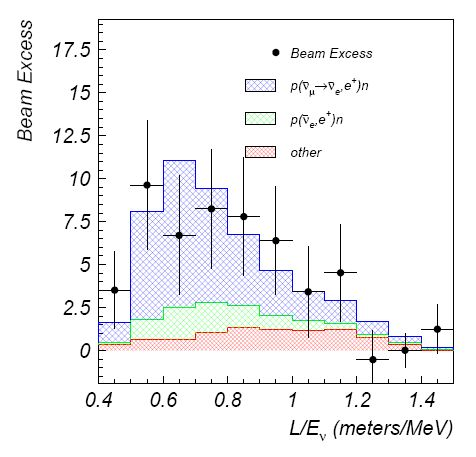
\includegraphics[width=.425\textwidth]{LSND_electrons_LoverE_dist}
      \hspace*{.5em}
      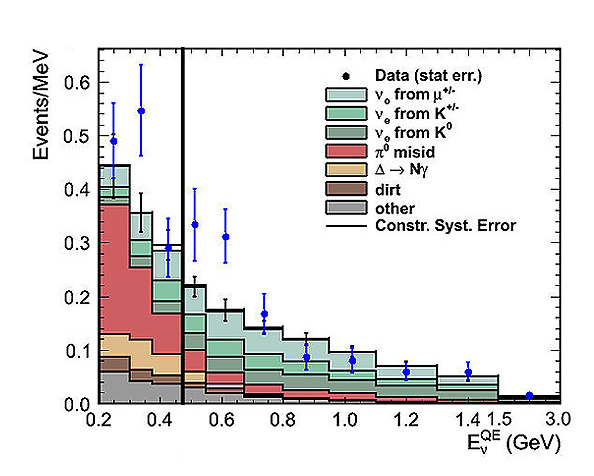
\includegraphics[width=.545\textwidth]{miniboone_excess_2}
    };
    \draw (-7.1,3.2) node[anchor=west, inner sep=1em, black] {\gls{lsnd}};
    \draw (.3,3.2)  node[anchor=west, inner sep=1em, black] {MiniBooNE};
  \end{tikzpicture}
  }
  \caption{%
    The plot on the left shows the beam excess observed by \gls{lsnd}.
    The blue region represents the required oscillation from $\bar{\nu}_\mu \to \bar{\nu}_e$.
    The plot on the right displays the excess of events at low energies observed by MiniBooNE.
  }
  \label{fig:anomaly_plots}
\end{figure*}

\subsection{MiniBooNE}

MiniBooNE was designed to observe neutrino oscillations and unambiguously verify or refute the \gls{lsnd} controversial result in a controlled environment.
The MiniBooNE detector was a Cherenkov detector located 541 m away from the target and was based on mineral-oil.\cite{Katori:2014qta}
The detector contained 800t of ultrarefined mineral oil and methylene compounds as scintillating liquid.
The experiment collected data for ten years from 2002 to 2012.

The results -- see figure \ref{fig:anomaly_plots} -- show an anomaly in the low energy distribution of the quasi-elastic neutrino events.
The observation indicate an excess of low energy electron-like events in \gls{ccqe}.\cite{Gninenko:2009ks}


\clearpage
\newpage

% The short baseline neutrino detector
\section{Short Baseline Neutrino Program}

Understanding the anomalies observed at \gls{lsnd} and MiniBooNE is one of the goals of the proposed \gls{sbn} program.
The program includes three \glspl{lartpc} located along the \gls{bnb} at Fermilab: \gls{sbnd}, MicroBooNE and Icarus.
This section aims to give an overview of the \gls{sbn} program beam and detectors.

\subsection{The Booster Neutrino Beam line}
The \gls{bnb} is one of the neutrino sources from Fermilab's Accelerator Complex, which comprises seven particle accelerators and storage rings\marginnote{including the main injector, \gls{numi}, the Tevatron, \ldots}.
The \gls{bnb} has successfully been operated for already 12 years in both neutrino and anti-neutrino modes.
The fluxes are well understood, systematic uncertainties associated with the beam have also been determined\cite[-.5em]{Antonello:2015lea}.
See figure \ref{fig:sbnp} for an overview of the location of the accelerators, detectors and the \gls{bnb} axis.
\begin{figure}
  \makebox[\textwidth]{%
  \begin{tikzpicture}
    % Map
    \node (img) {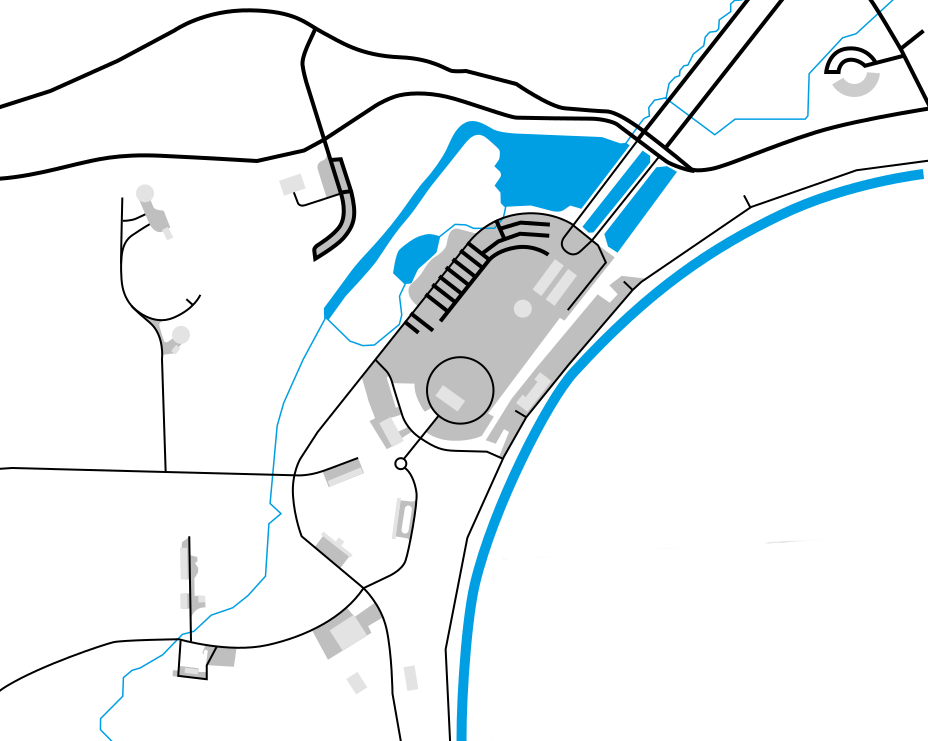
\includegraphics[width=\textwidth]{maps_fermilab_cutout}};
    % Accelerators
    \draw[solarized-red, very thick, densely dotted] ( -.05, -.225) circle (.4cm);
    \begin{scope}
      \clip(-6,-4.25) rectangle (3, 3);
      \begin{scope}[rotate=30]
        \draw[solarized-base0, very thick, densely dotted] (-5.9, -4.25) ellipse (2.6cm and 3.3cm);
      \end{scope}
    \end{scope}
    \draw[solarized-red, very thick, densely dashed] (-.45, -.225) -- (-.4, -1.55);
    \begin{scope}
      \clip(-2.4, -1.55) rectangle (2, -4);
      \draw[solarized-red, very thick, densely dashed] (-2.4, -1.55) circle (2cm);
    \end{scope}
    \begin{scope}
      \clip(-2.4, -2.8) rectangle (-4, -4);
      \draw[solarized-red, very thick, densely dashed] (-2.4, -2.8) circle (.75cm);
    \end{scope}
    % Target
    \draw[solarized-red,  very thick] (-3.15, -2.5) circle (.25cm);
    \draw (-3.15,-2.5) node[cross=.24cm, solarized-red, very thick] {};
    % Detectors
    \draw[solarized-blue, very thick] (-3.19, -1.7) circle (.2cm);
    \draw[solarized-magenta, very thick] (-3.3, .4) circle (.2cm);
    \draw[solarized-base0,very thick] (-3.3, .95) circle (.2cm);
    \draw[solarized-cyan,very thick] (-3.37, 1.3) circle (.2cm);
    \draw[solarized-base0,very thick,densely dashed] (-3.6, 1.9) circle (.3cm);
    % Beam lines
    \draw[solarized-blue, dashed, very thick, ->] (-3.175,-2.1) -- (-3.55, 4.2);
    \draw[solarized-base0, dashed, very thick, ->] (-1.5,-3.2) -- (-4.5,3.9);
    % Legende
    \draw[solarized-red, very thick, densely dotted] (1.5, -1)   circle (.15cm)
      node[anchor=west, inner sep=1em, black] {Booster Ring};
    \draw[solarized-red,very thick, densely dashed] (1.4, -1.6) -- (1.6, -1.4);
    \draw (1.5,-1.5) node[anchor=west, inner sep=1em, black] {Proton beam};
    \draw (1.5,-2) node[cross=.4em, solarized-red, very thick] {};
    \draw[solarized-red,  very thick] (1.5,-2) circle (.15cm)
      node[anchor=west, inner sep=1em, black] {Target \& decay pipe};
    \draw[solarized-blue,very thick, dashed, ->] (1.4, -2.6) -- (1.6, -2.4);
    \draw (1.5, -2.5) node[anchor=west, inner sep=1em, black] {\gls{bnb} axis};
    \draw[solarized-blue,   very thick] (1.5,-3.125)   circle (.15cm)
      node[anchor=west, inner sep=1em, black] {\gls{sbnd}};
    \draw[solarized-magenta, very thick] (1.5,-3.625) circle (.15cm)
      node[anchor=west, inner sep=1em, black] {MicroBooNE};
    \draw[solarized-cyan, very thick] (1.5,-4.125)   circle (.15cm)
      node[anchor=west, inner sep=1em, black] {Icarus};
  \end{tikzpicture}
  }
  \caption{%
    Traced map of Fermilab and the detectors involved in the \gls{sbn} program.
    The Main Injector, MiniBooNE, Minos, Minerva, Nova and the \gls{numi} axis were added as reference points.
  }
  \label{fig:sbnp}
\end{figure}

The beam's starting point is the radio-frequency quadrupole accelerator, which accelerates and separates the protons into bunches.
Then the protons pass through a 150m linear accelerator before they're fed to the Booster Ring.
After reaching energies of 8.89GeV in the ring the protons are guided to the beryllium target.
The target measures 71cm long\marginnote{The length of the target corresponds to 1.7 interaction lengths.} and is only 1cm in diameter.
The resulting charged particles are focused using a magnetic horn and decay in a 50m long region filled with air\marginnote{Commonly known as the decay pipe.}, where the \gls{bnb} is generated.
This region can be shortened to 25m with the use of an absorber to influence the resulting flux.

\subsection{MicroBooNe}

MicroBooNE is the first operative \gls{lartpc} detector of the \gls{sbn} program.
The observation of tracks started in August 2015 and the collaboration is already taking and registering data.
Figure \ref{fig:events_microboone} displays some neutrino event candidates observed at MicroBooNE.

\begin{figure}
  \centering
  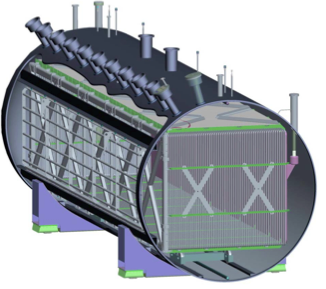
\includegraphics[width=.42\textwidth]{microboone_scheme}
  \caption{Scheme of the \gls{lartpc} of MicroBooNE}
  \label{fig:microboone_concept}
\end{figure}

MicroBooNE's active mass is 89 tons and its \gls{lartpc} is contained in a cryostat.
The active region is a rectangular volume of dimensions $2.33m \times 2.56m \times 10.37m$.
The cathode is situated at the boundary of the active volume on the left beam side of the detector.
The design of the chamber allows the ionization electrons of the charged particle tracks' to drift up to 2.56m to the wire grids, where the readout is made in the right beam side of the detector.
\Glspl{pmt} are installed behind the read out wire planes to collect prompt scintillation light produced in the argon.

\subsection{Short-Baseline Near Detector}

\begin{figure}
  \centering
  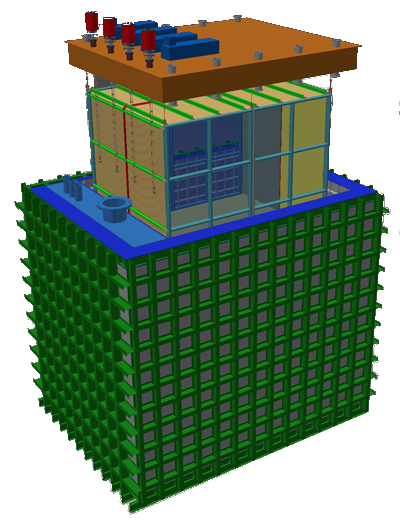
\includegraphics[width=.36\textwidth]{sbnd_detector_concept_new}
  \caption{Scheme of the \gls{sbnd}}
  \label{fig:sbnd_concept}
\end{figure}

The \gls{sbnd} is a \gls{lartpc} in contruction with an active volume of $4m \times 4m \times 5m$ at 110 meters from the \gls{bnb} target -- figure \ref{fig:sbnd_concept} illustrates its building concept.
The \gls{lartpc} has a capacity for 112 tons of liquid argon and is contained in a membrane-style cryostat.
It features four anode plane assemblies for signal readout.
The maximal drift distance of the ionization electrons is 2m, $\approx$20\% shorter than the maximal drift length in MicroBooNE.
\Gls{sbnd} will additionally feature a light collection system for detecting the scintillation light produced in the argon volume.
The operation of the \gls{sbnd} is planned to start in 2018.


\clearpage
\newpage

\section{Electron neutrino signals from cosmic background}
A flux of particles from outer space constantly bombards the Earth's atmosphere, generating an important background signal in \glspl{lartpc}, the main reason for the construction of the \gls{crt}.
This section handle \glspl{cr} and the associated effects that contribute to neutrino signal..
\label{sec:cosmics}

\subsection{Cosmic rays}
Cosmic rays were discovered nearly a century ago and its origin and composition is not yet fully understood.
The energy range of these incident particles is very wide, reaching ultra high energies above $10^{8}$GeV, whose origin is still unknown\cite[-8em]{Dova:2016ipa}.
These cosmics travel millions of light years to before they reach earth, reason for which only stable particles are observed.
Due to observed charges of these particles, the sources of these primary cosmic rays are assumed to be of electromagnetic nature.

\begin{figure}
  \centering
  \makebox[.45\textwidth]{
  \begin{tikzpicture}
    % Map
    \node (img) {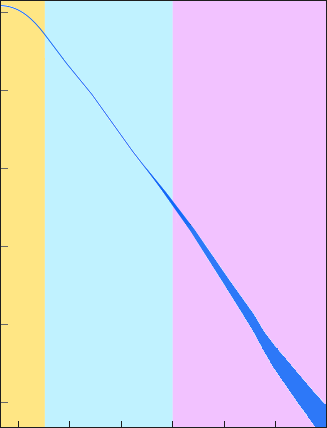
\includegraphics[width=.45\textwidth]{cosmics}};
 
    % Y-Axis
    \draw (-2.25,-2.85 ) node[anchor=east, inner sep=1em] {$10^{-27}$};
    \draw (-2.25,-1.7  ) node[anchor=east, inner sep=1em] {$10^{-21}$};
    \draw (-2.25,-.45  ) node[anchor=east, inner sep=1em] {$10^{-15}$};
    \draw (-2.25, .7   ) node[anchor=east, inner sep=1em] {$10^{-9}$};
    \draw (-2.25,1.95  ) node[anchor=east, inner sep=1em] {$10^{-3}$};
    \draw (-2.25,3.1   ) node[anchor=east, inner sep=1em] {$10^{3}$};
 
    \node[label={[label distance=0.5cm,text depth=-1ex,rotate=90]above:$F \quad (m^{-2} \text{sr}^{-1} s^{-1} \text{GeV}^{-1})$}] at (-3.1,0) {};
 
    % X-Axis
    \draw (-2.3,-2.8) node[anchor=north, inner sep=1em] {$10^0$};
    \draw (-1.5,-2.8) node[anchor=north, inner sep=1em] {$10^2$};
    \draw (- .7,-2.8) node[anchor=north, inner sep=1em] {$10^4$};
    \draw (  .1,-2.8) node[ anchor=north, inner sep=1em] {$10^6$};
    \draw (  .9,-2.8) node[  anchor=north, inner sep=1em] {$10^8$};
    \draw ( 1.7,-2.8) node[ anchor=north, inner sep=1em] {$10^{10}$};
    \draw ( 2.5,-2.8) node[ anchor=north, inner sep=1em] {$10^{12}$};
    
    % Label
    \draw (.1,-3.6) node[anchor=north, black] {$E \quad (\text{GeV})$};
  \end{tikzpicture}
  }
  \caption{%
    This plots displays the flux of cosmic rays in dependency of the particle's energy.
    The colored regions denote the particle fluxes:
    $1 \text{m}^{-2}\text{s}^{-1}$ (yellow),
    $1 \text{m}^{-2}\text{yr}^{-1}$ (cyan),
    $1 \text{km}^{-2}\text{yr}^{-1}$ (magenta).
  }
  \label{fig:cosmics}
\end{figure}

Using balloon-borne and space-based experiments the energy spectrum and components of \gls{cr} have been studied\cite{Maestro:2015lla}.
The most abundant components of cosmic radiation are protons and helium nuclei.
Elements of atomic number greater than \ce{Fe} are extremely rare.

\begin{figure}
  \centering
  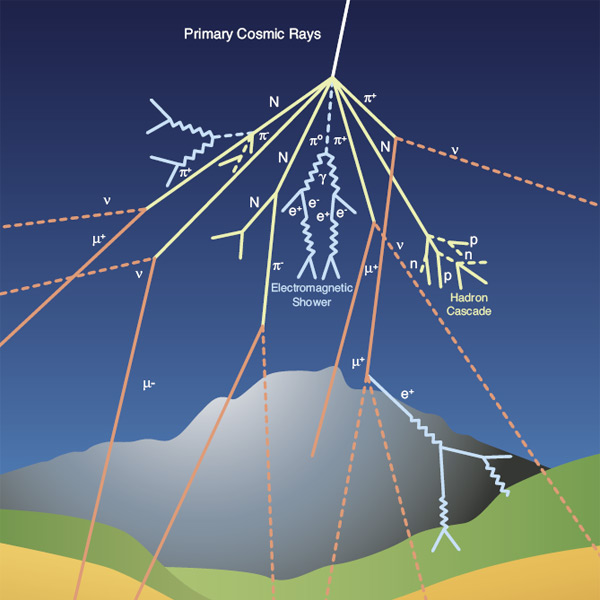
\includegraphics[width=.9\textwidth]{cosmic_ray}
  \caption{%
    A primary cosmic ray interacts in the atmosphere and produces a shower of particles as illustrated.
  }
  \label{fig:particle_shower}
\end{figure}

Cosmics contribute to the neutrino signal, due to the production of electromagnetic and hadronic showers of the constituents of the primary and subsequent cosmic rays.
Electromagnetic showers involve many photons which can contribute to the neutrino signal.
Hadronic showers result in neutral pions, which decay to high energy photons shortly after production.

\subsection{Interactions contributing to the neutrino signal}

Besides of the backgrounds contributed by the neutrino fluxes discussed in the section on neutrino sources, signal contributions of the high energy photons in these showers need to be taken into account.

The main contributions to the neutrino signal are given by compton scattering events and electron positron production.
Photons are not visible in the \gls{lartpc}'s signal, the resulting free electrons from the photon interactions cannot be distinguished from a free electron of a neutrino interaction.
See figure \ref{fig:cosmics_interactions} for an illustration.
\begin{figure}
  \centering
  \vspace{1em}
  \begin{fmffile}{sc}
    \begin{fmfgraph*}(135,100)
      \fmfleft{i1}
      \fmfright{o1,o2}
      \fmf{photon}{i1,v1,o1}
      \fmf{fermion}{v1,o2}
      \fmflabel{$\gamma$}{i1}
      \fmflabel{$\gamma$}{o1}
      \fmflabel{$e^-$}{o2}
    \end{fmfgraph*}
    \hspace*{2em}
    \begin{fmfgraph*}(135,100)
      \fmfleft{i1}
      \fmfright{o1,o2,o3}
      \fmf{phantom}{i1,v1,v2,o1}
      \fmf{photon}{i1,v1}
      \fmf{fermion}{v2,v1,o1}
      \fmf{photon}{v2,o2}
      \fmf{photon}{v2,o3}
      \fmflabel{$\gamma$}{i1}
      \fmflabel{$\gamma$}{o2}
      \fmflabel{$\gamma$}{o3}
      \fmflabel{$e^-$}{o1}
    \end{fmfgraph*}
  \end{fmffile}

  \caption{%
    Compton scattering is displayed on the left.
    Pair production with subsequent annihilation of the positrion with an electron of the medium is displayed on the right.
  }
  \label{fig:cosmics_interactions}
  \vspace{1em}
\end{figure}

The contribution of Compton scattered electrons to the electron neutino signal is comprehensible.
In the case of electron-positron pair production, the subsequent annihilation of the positron with an electron in the medium is required, to interpret the event as a neutrino interaction.



\clearpage
\newpage

% - How to build the CRT
\section{The Cosmic Ray Tagger}
Detecting and tracing incident ionizing background radiation to distinguish background from a \gls{bnb}-based event in the \gls{lartpc} is the main goal of the \gls{crt}.
This section covers the \gls{crt} modules functionality and important parameters are listed.

\subsection{The Cosmic Ray Tagger in a nutshell}
If the times and positions at which an incident particle entered and exited our detector are known, we can identify the crossing particle's trace.
To trace incident radiation in a \gls{tpc}, the latter needs to be covered with an additional detector generating a grid.
This additional detector is the \gls{crt} and a scheme of it is illustrated in figure \ref{fig:scheme}.

\begin{figure}
  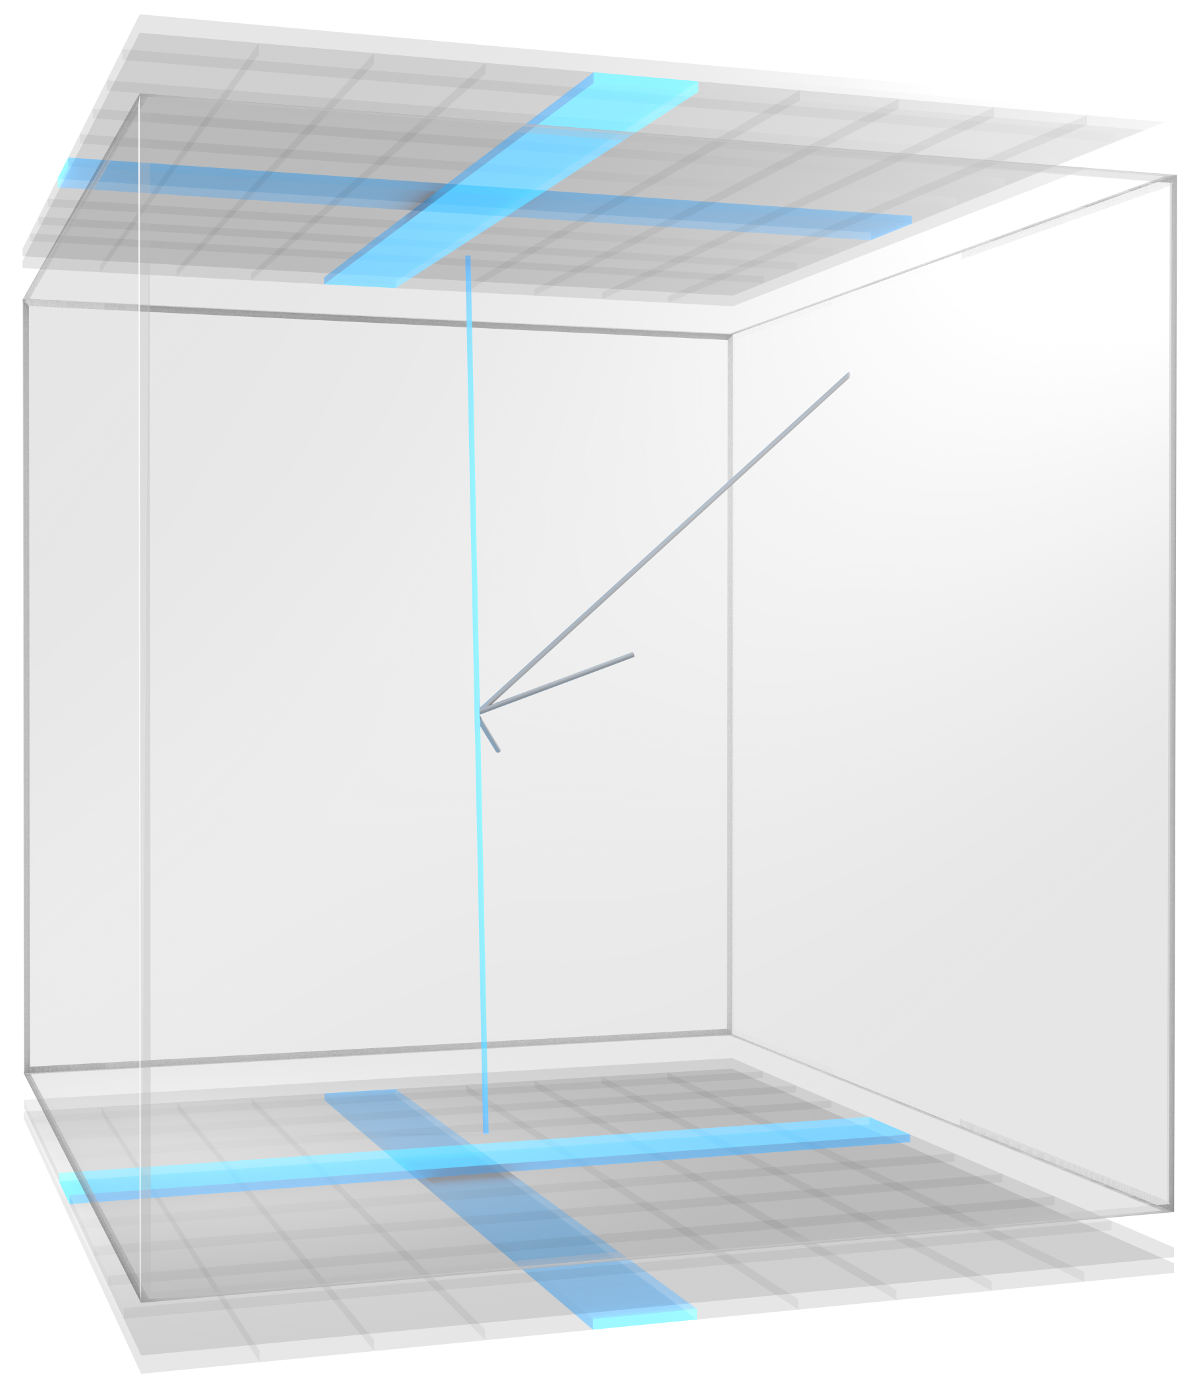
\includegraphics[width=.9\textwidth]{detector}
  \caption{%
    Schematic of two layers of \gls{crt} positioned above and below a virtual \gls{tpc} containing an event.
    The event represents the interaction between a muon neutrino and a proton ($\nu_\mu + p \to p' + \pi^+ + \mu$) with an atmospheric muon travelling close to the event's vertex.
    The highlighted scintilating bars are crossed by the atmospheric muon.
    Using the grid produced by the scintilating bars the atmospheric muon's path can be identified.
  }
  \label{fig:scheme}
\end{figure}

The \gls{crt} consists of several independent detectors (modules), making it fully modulable.
Each \gls{crt} module consists of a \gls{crt} panel and a \gls{feb}, which processes the panel's incoming signals to event data.
A layer of \gls{crt} requires at least two panels -- to generate a grid of scintillating pixels -- and two layers are needed to track incident particles.
If the position of the panels is well known, their signals and time coincidence can be used to determine the entry and exit points of the incident particle.

\subsection{Background mitigation}

Charged particles will generate a signal in our \gls{crt} modules.
Using these signals, a cylindrical volume can be constructed around the path of the incident particles.
This volume acts as a veto for the track.

If the vertex of a neutrino event is inside the veto region, the event needs to be reconstructed with more delicate algorithms to distinguish the neutrino signal from the cosmic signal.
The following parameters of the detector are of severe importance to achieve a useful veto signal with the smallest possible volume..

\paragraph{Time resolution} The time a particle takes to cross our detector is given by the particle's velocity.
If the \gls{crt} modules are run without using the coincidence signals featured by the \gls{feb}, these coincidences need to be reconstructed from the detector data.
A precise time resolution is required for this task.

\paragraph{Position resolution} is principally given by the width of the bars installed in the module.
This resolution can be improved by calibrating the signal ratio and signal amplitudes for the channels of a bar.

\paragraph{Detection efficiency} Not every occurrent particle transition is registered as an event by our detector.
Many physical effects\marginnote{Quantum efficiencies, geometrical fill factors, surface reflections, detection ranges, signal losses\ldots} influence the particle detection efficiency of the \gls{crt}.
An important contribution to detection efficiency is made by the set threshold, since it will change the part of the energy spectrum observed by the \gls{crt}.

\clearpage
\newpage

% - How to build the CRT
\section{The Cosmic Ray Tagger panel}

This section covers technical aspects of the panels' components as well as manufacturing processes.

\subsection{The panel in a nutshell}
A panel consists of 16 scintillating bars embedded in an aluminium cover.
Each of the bars is prepared with two grooves, two \gls{wlsf}, a plastic endpiece and an electronics board with two embedded \gls{sipm}.
See figure \ref{fig:exploded_bar} for assembled and exploded assembly drawings of the scintillating bar.

\begin{figure}
  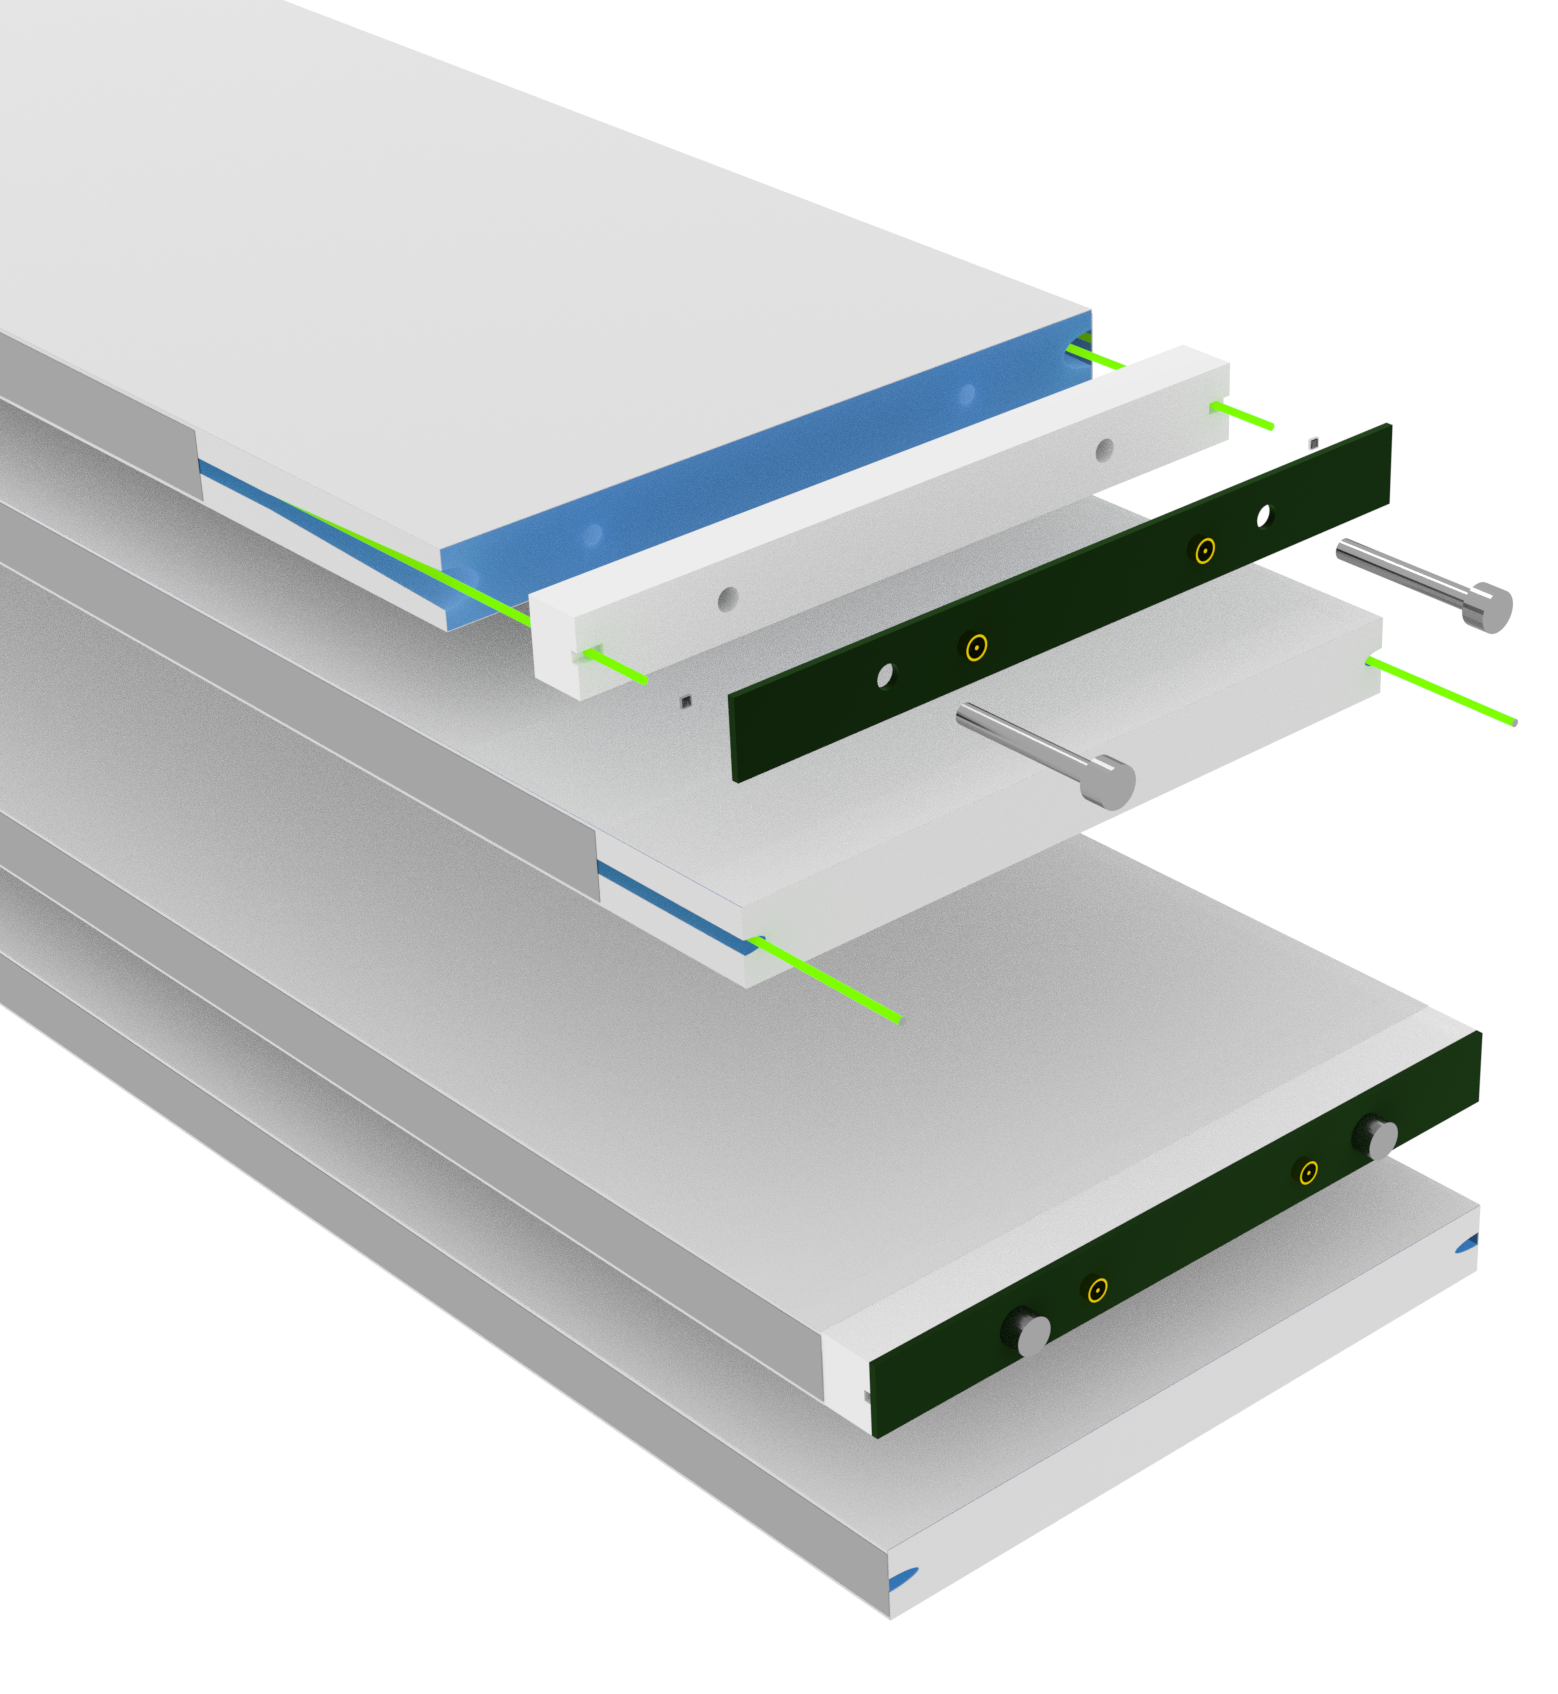
\includegraphics[width=\textwidth]{assembly}
  \caption{%
    Assembled and exploded views of front and rear ends of scintillating bars.
    The long sides of the bars (blue) are furnished with grooves containing the \glspl{wlsf} (fluorescent green) to guide the scintillation light to the \glspl{sipm} (black).
    The grooves are covered with mylar foil (gray).
    The plastic endpiece (white) serves as a physical guide and holder for the \glspl{wlsf}.
    The electronics and the enpiece are fixed to the bar with screws.
    Optical glue keep the \glspl{wlsf} and the mylar foil in place.
  }
  \label{fig:exploded_bar}
\end{figure}

When a high energy particle traverses the panel, it will most likely cross one of the scintillating bars\marginnote{This likelyhood depends on the fill factor of the panel} and induce the isotropical emission of photons.
These photons will be attenuated along their path in the material and reflected on the bars' walls until some of them reach the \gls{wlsf}.
The \gls{wlsf} are used for their light propagation properties and low attenuation coefficient, which allow some of the fluorescense photons to reach the \glspl{sipm}.
The photons arriving to the \gls{sipm} may induce the discharge of a cell in the \gls{sipm}, generating an observable signal.

\subsection{Aluminium shielding} The bars are covered with sheets of aluminium to shield the scintillating plastic and \glspl{sipm} from photons and charged particles.
The aluminium cannot dissipate all particle's energy, letting some photons and high energy particles through.
Knowing the kind of radiation tresspassing the detector is insightful, this is discussed for photons and charged particles.

\paragraph{Photons} are attenuated exponentially by the material along their path
\begin{equation*}
  I(x) = I_0 e^{-\mu x},
\end{equation*}
where $I_0$ is the intensity of the transmitted radiation at the interface and $x$ the perpendicular distance from the interface.

The attenuation depends on the energy of the photons, the nuclear structure and density of the material.
The attenuation coefficients for aluminium are displayed in figure \ref{fig:attenuation_coefficient_alu}.
\begin{figure*}
  \centering
  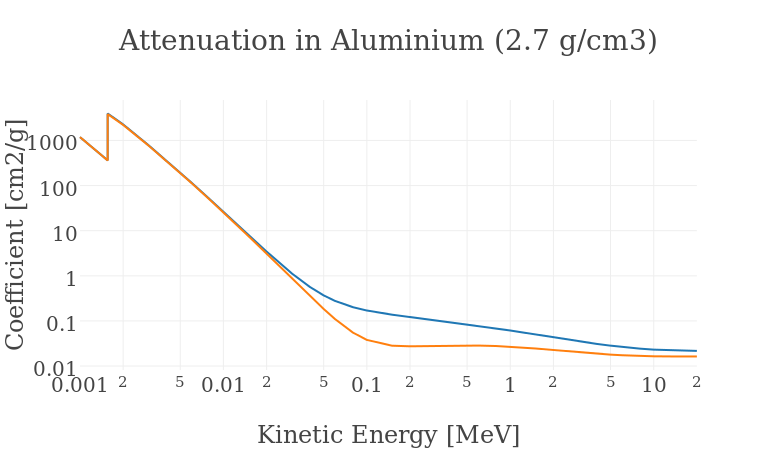
\includegraphics[width=.48\textwidth]{shielding/attenuation_photon}
  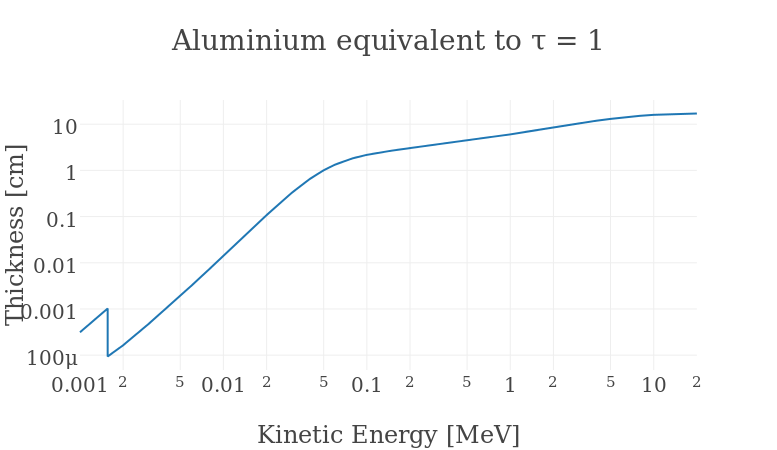
\includegraphics[width=.48\textwidth]{shielding/optical_depth}
  \caption{%
    The plot on the left displays the attenuation coefficient (blue) and energy absorption coefficient (orange) for photons in aluminium.
    The right plot displays the thickness of aluminium required to have an optical depth of one.
    Data used from NIST tables.
    Data source: \href{http://physics.nist.gov/PhysRefData/XrayMassCoef/tab3.html}{NIST Xray Mass Coefficients},
  }
  \label{fig:attenuation_coefficient_alu}
\end{figure*}

Since single photons can reach great depths in any material, it is more commonly used to express the thickness of a layer of material for incident radiation in optical depth
\begin{equation*}
  \tau = \mu x,
\end{equation*}
where $\mu$ is the attenuation coefficient and $x$ the thickness of the layer of material.

\marginnote{Assuming photons of the energy of 1.5MeV -- which is approximately the energy of the $\gamma$ photons resulting from \ce{^40K} undergoing electron capture in ambient radiation -- the mass attenuation coefficient of aluminium is $\mu_\rho = 0.05 \text{cm}^2 \text{g}^{-1}$ and therefore $\mu = \mu_\rho \rho = 0.135 \text{cm}^{-1}$.
The optical depth of $\tau = 1$ is reached with a $x = \frac{1}{\mu} = 7.4cm$ thick layer of aluminium.
For photons of energies above 0.1MeV, 2mm of aluminium is almost transparent.
}

\paragraph{Charged particles} For charged particles the penetration range can be estimated using a continuously slowing down approximation and the stopping powers of aluminium for every kind of particle
\begin{align*}
  R(E_0) &= \int_{E_0}^{0} \frac{1}{S(E)} dE \\
         &= \int_{E_0}^{0} -\frac{dx}{dE} dE.
\end{align*}

The high stopping power of aluminium for charged hadronic radiation stops heavy charged particles.
The nuclear contribution to energy loss for charged hadronic radiation is negligible.
Electrons lose almost all their kinetic energy to other electrons.
The radiation contributions of electrons start to be significant only for kinetic energies above 50MeV.
Using the stopping powers the ranges inside aluminium in depedence of their energy can be computed.
See figure \ref{fig:shielding} for an illustration of the stopping powers and ranges for electrons, protons and alpha particles in aluminium.

\begin{figure*}
  \centering
  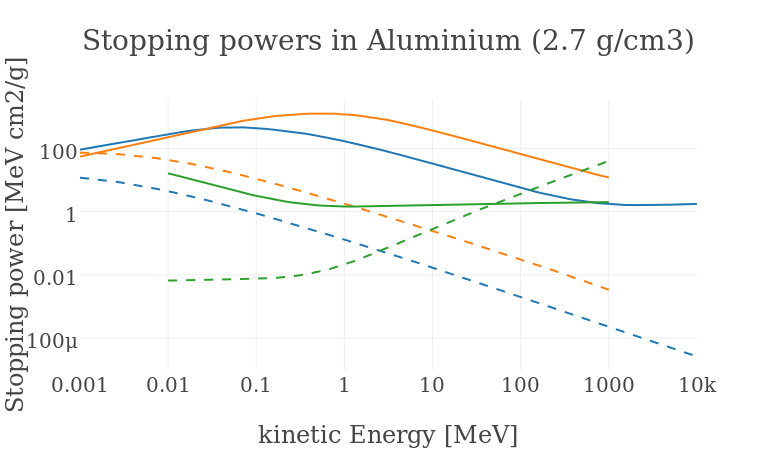
\includegraphics[width=.48\textwidth]{shielding/stopping_powers}
  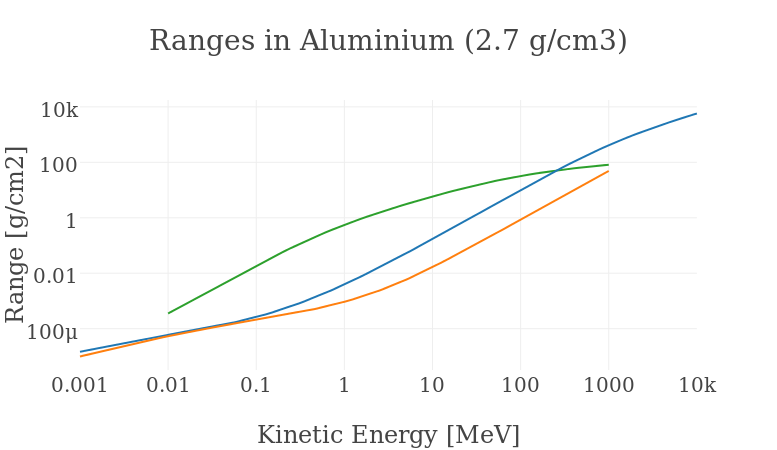
\includegraphics[width=.48\textwidth]{shielding/csda_ranges}
  \caption{%
    The stopping powers (left) and \gls{csda} ranges (right) are displayed for electrons (green), protons (blue) and alpha particles (orange).
    The radiative energy losses for electrons and nuclear contributions for the hadros are dashed.
    Data source: \href{http://physics.nist.gov/PhysRefData/Star/Text/ESTAR.html}{NIST ESTAR},
                 \href{http://physics.nist.gov/PhysRefData/Star/Text/PSTAR.html}{NIST PSTAR} \&
                 \href{http://physics.nist.gov/PhysRefData/Star/Text/ASTAR.html}{NIST ASTAR}
  }
  \label{fig:shielding}
\end{figure*}

\subsection{Scintillating bars}
The scintillating bars generate the grid of the \gls{crt} and yields light from the incident radiation.
A scintillator is a material which emmits light through luminescence when exposed to radiation.
When struck by ionizing radiation, a scintillator will absorb some of the radiation's energy and release the absorbed energy by light emission.\marginnote[2em]{Luc Beaulieu gave a good review on \href{https://vimeo.com/76977696}{Plastic Scintillation Detectors} at the AAPM 2013.}

The scintillation light originates from an organic fluor which is mixed into the plastic out of which the bars are produced.
The fluor excites into a metastable state, but its decay time is short\marginnote{The decay time is of the order of nano seconds.}, leading to almost no delay on the emission of the scintillation light.
The scintillation light is emitted isotropically from the radiation's incident point.
The components of the scintillating plastic are listed on table \ref{tab:material_safety_data_sheet}, the spectra of absorption and fluorescence of the scintillating components are displayed in figure \ref{fig:scintillator_graphs}.

\begin{table}
  \centering
  \begin{tabular}{ l l c }
    Ingredient                          & Synonym     & \% WT \\
    \hline
    Styrolution PS GPPS                 &             & 98.46 \\
    1,4-Diphenylbenzene                 & p-Terphenyl & 1.5   \\
    1,4-Bis(5-phenyl-2-oxazolyl)benzene & POPOP       & 0.04  \\
    \hline
    \\
  \end{tabular}
  \caption{%
    Composition / Information on ingredients of the scintillating plastic used for the bars of the \gls{crt}.
  }
  \label{tab:material_safety_data_sheet}
\end{table}

The bars come prepared with a thermal treatment, which increases the reflexion of light.
The size of the bars vary, depending on the dimensions of the module they are built in.
One side of the bars is faced to have a clean interface to fix the plastic endpiece to.
The grooves need to be cut open before glueing the \gls{wlsf} into them.

\begin{figure*}
  \centering
  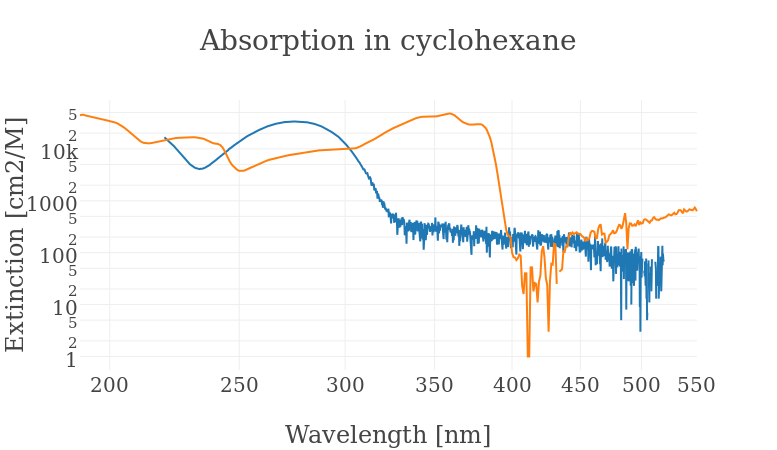
\includegraphics[width=.48\textwidth]{scintillators/absorptions_thin}
  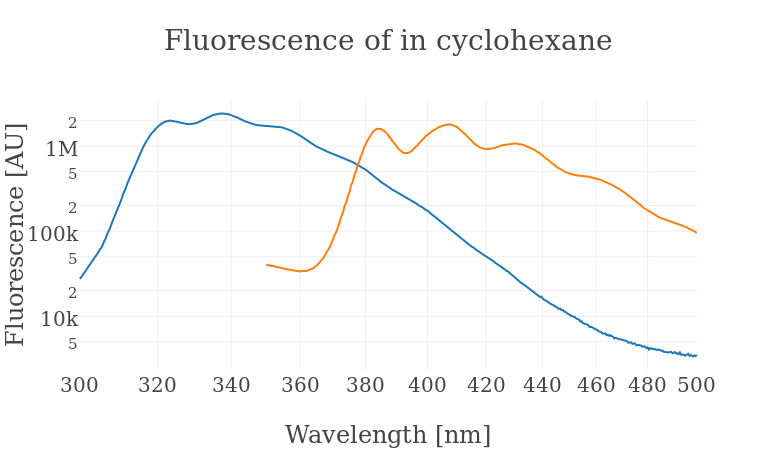
\includegraphics[width=.48\textwidth]{scintillators/fluorescences_thin}
  \caption{%
    (fttb)
    Optical absorption and fluorescence emission spectrum of p-Terphenyl (blue) and POPOP (orange) in cyclohexane.
    Data from PhotochemCAD package, version 2.1a (Du 1998, Dixon 2005), http://omlc.org/spectra/PhotochemCAD/
  }
  \label{fig:scintillator_graphs}
\end{figure*}

The scintillating bars are fixed to the aluminium sheets using double sided scotch tape.
The short sides of the panels are fixed to a prepared aluminium bar with screws.
The long sides of the panels are closed with U-shaped aluminium profiles, which are fixed with glue to the rest of the panel.
The gaps that might arise are closed with glue to minify the transision of photons.


\subsection{Wavelength shifting fibers}
Since light is collected through the fiber's cladding and a very low attenuation coefficient is needed, a \gls{wlsf} is used to guide the light from the scintillating bar to \glspl{sipm}.
\gls{wlsf} are very efficient light guides, since their emission and absorption spectrum is shifted, which leads to a very low attenuation coefficient.
The absorption and emission spectrum and the attenuation of the spectrum along a fiber are displayed on figure \ref{fig:wlsf_observations}.
Further technical details for the \gls{wlsf} Y-11 can be found on \href{http://kuraraypsf.jp/psf/ws.html}{kuraray's website} and its product catalogue.

\begin{figure*}
  \centering
  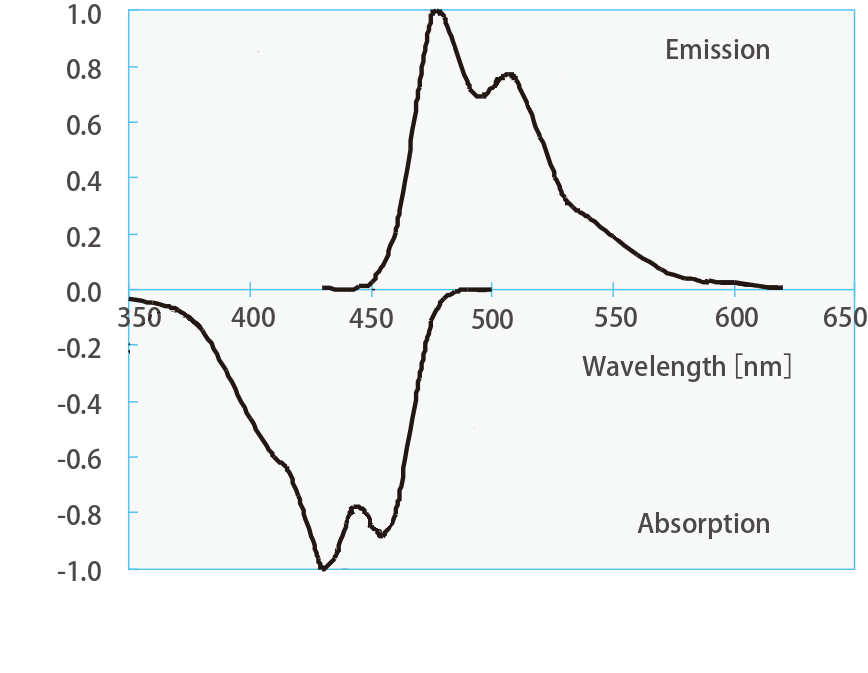
\includegraphics[width=.427\textwidth]{wlsf/absorption_emission_y11.png}
  \hspace*{1em}
  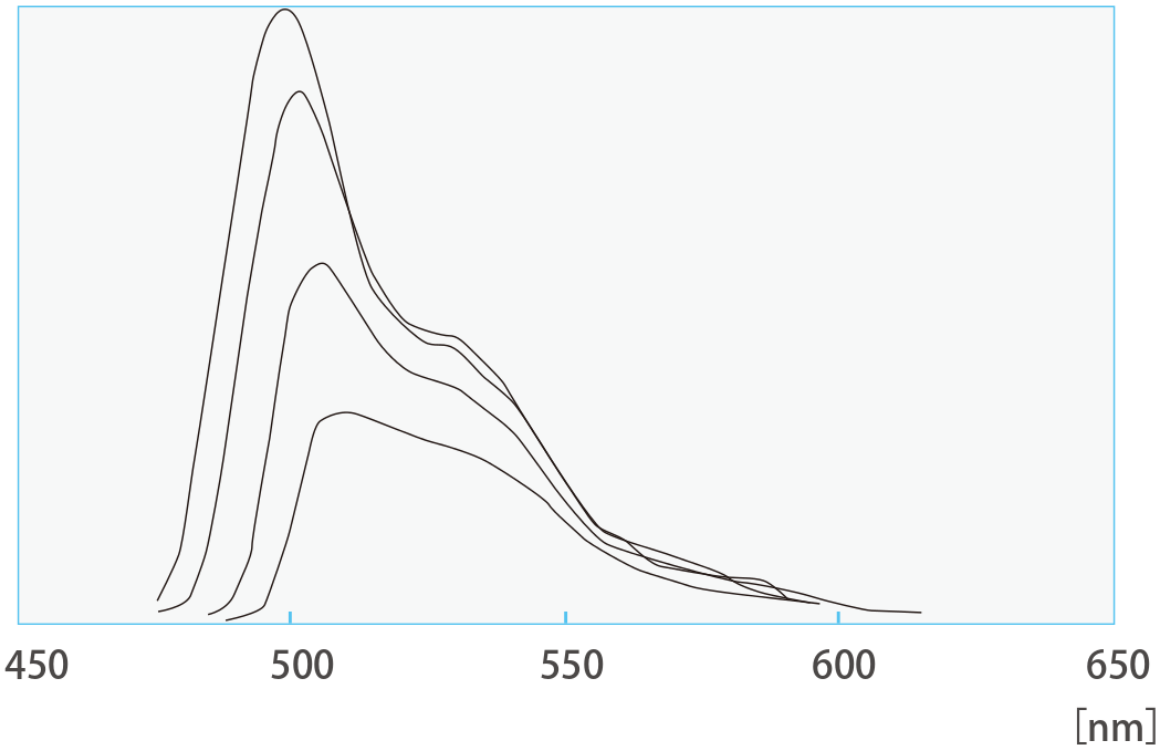
\includegraphics[width=.515\textwidth]{wlsf/attenuation_y11.png}
  \caption{%
    Absorption and emission spectrum of the \glspl{wlsf} displayed on the left shows peaking fluorescence emission at 476 nm and a maximal absorption at 430 nm.
    Attenuation of the spectrum of the \glspl{wlsf} on the right displays the spectrum at different distances (fttb 10, 30, 100, 300cm) from the source's incident point.
    The used light source to excite the fibers had a wave length of 430nm.
    Source: \href{http://kuraraysf.jp/pdf/all.pdf}{kuraray's product catalogue}
  }
  \label{fig:wlsf_observations}
\end{figure*}

The fibers are cut according to the length of the bars.
Both ends of the fibers are faced using a diamond-cutter to optimize the interface.
Aluminium is evaporated on the far end, to improve the reflexion of light.
The uncoated end is put on top of the \gls{sipm}, by using the plastic endpiece as physical guide and holder.
The fibers are glued to the groove using optical glue.

% Method
%\begin{figure*}
%  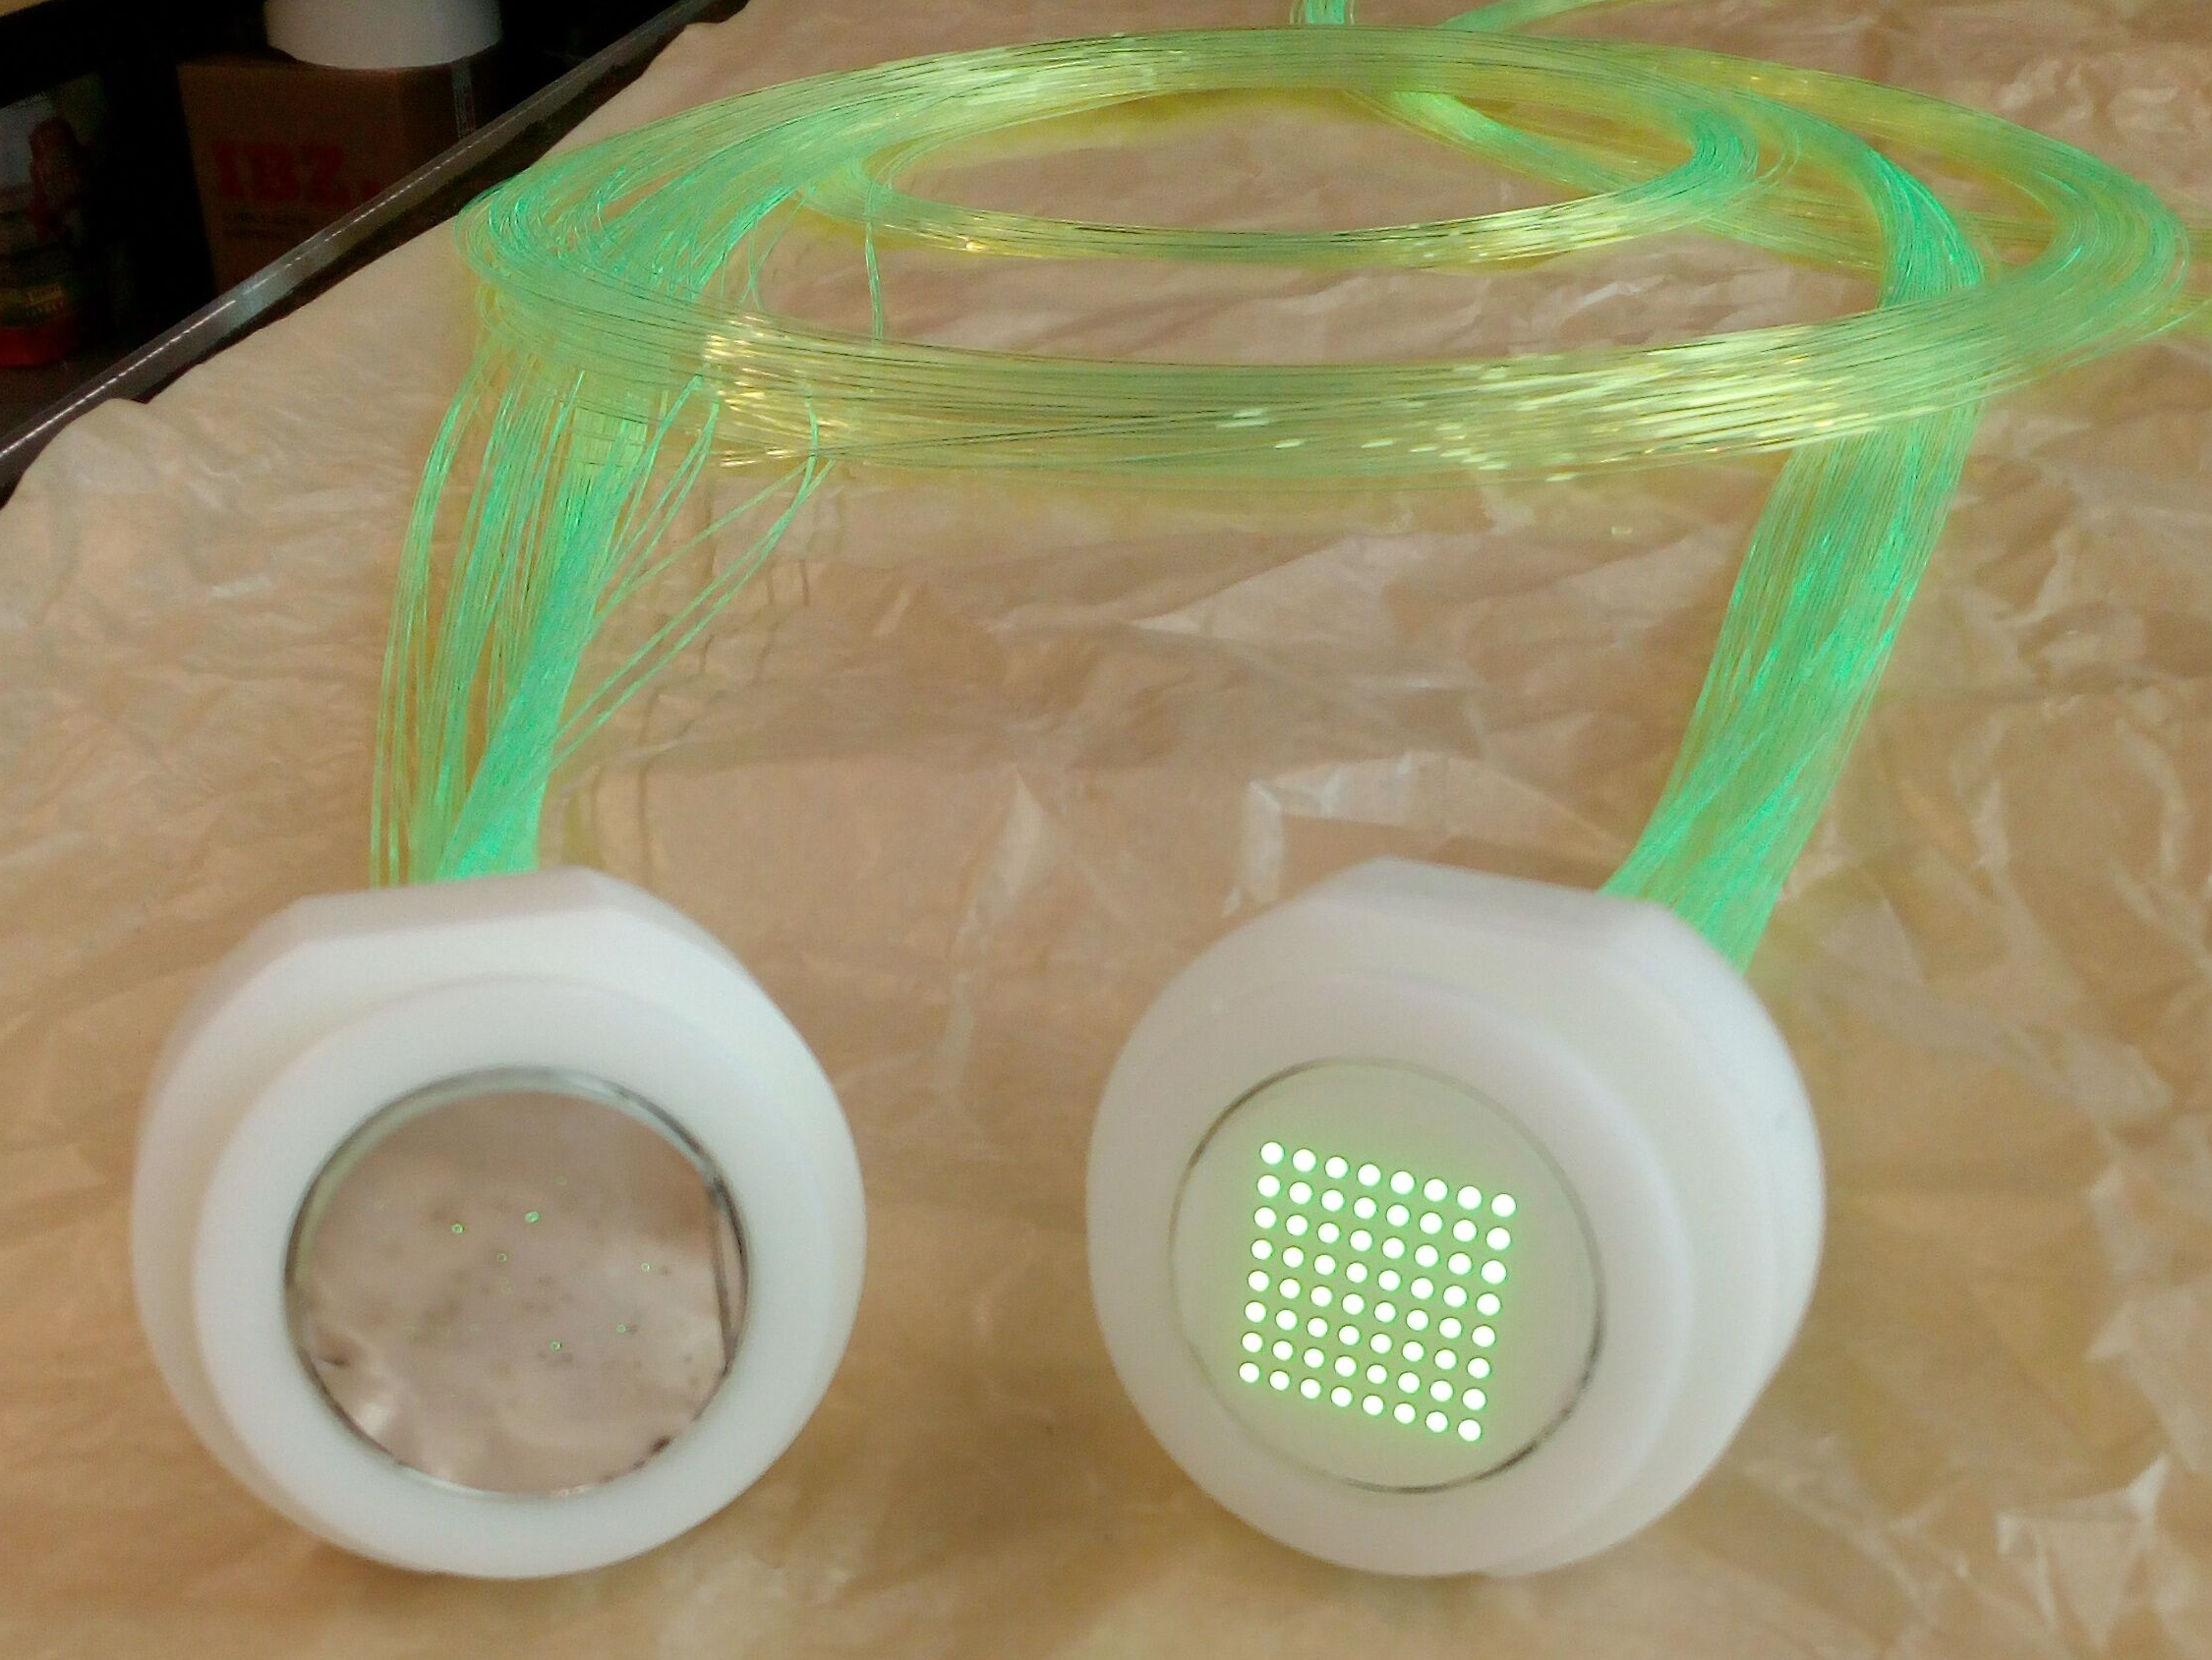
\includegraphics[width=\textwidth]{wlsf/fibers}
%  \caption{%
%    Fibers ready for assembly.
%    The fibers are fixed into plastic nests with optical glue, then both ends are diamond-cut.
%    One end is evaporated with aluminium to increase light reflexion.
%  }
%  \label{fig:exploded_bar}
%\end{figure*}
\clearpage
\subsection{Silicon photomultiplier}

A \gls{sipm} is an array of cells made of silicon, a well known semiconductor which is able to carry electrons and electron holes.
Each cell of the \gls{sipm} behaves like a diode, the electronic equivalent of a \gls{sipm} is displayed in figure \ref{fig:sipm_array_diodes}.

\begin{figure}
  \centering
  \begin{circuitikz}
    \node[ground] (g1) at (0, -1) {};
    \draw (0, -1) to[V=$V_\text{bias}$] (0, 1);

    \draw (0, 1) -- (1, 1);
    \draw (4, 1) to[D] (2.5, 1) to[R] (1, 1);
    \draw (4, 0) to[D] (2.5, 0) to[R] (1, 0) -- (1, 1);
    \draw (4, -1.5) to[D] (2.5, -1.5) to[R] (1, -1.5);
    \draw (1, 0) -- (1, -.5);
    \draw[densely dotted] (1, -.5) -- (1, -1);
    \draw (1,-1) -- (1,-1.5);

    \draw[densely dotted] (4, -.5) -- (4, -1);
    \draw (4, 1) -- (4, -.5);
    \draw (4, -1) -- (4,-1.5);
    \draw (4, 1) to[short,-o] (4.5, 1);
    \draw (4.5, 1) node[right] {$S_i$};

  \end{circuitikz}
  \caption{%
    Each branch of this electronic scheme represents a cell of the \gls{sipm}.
    All cells of the same crystal share the same bias voltage.
  }
  \label{fig:sipm_array_diodes}
\end{figure}

The charge carriers in the cells' silicon latice can be knocked out by incoming photons and drift to their appropiated electrodes if a field is applied.
With greater field the drift velocity increases, to the point where further charged carriers are knocked out.
With a sufficiently high voltage\marginnote{also called breakdown voltage} a photo electron leads to a self-sustaining avalanche.
A typical structure of a cell is shown in figure \ref{fig:sipm_structure}.

\begin{figure}
  \centering
  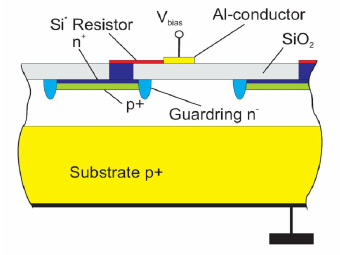
\includegraphics[width=.6\textwidth]{sipm_structure}
  \caption{%
    Typical structure of a \gls{sipm}'s cell.
    The cells are generally arranged on a 2 dimensional array.
    -- \copyright M. Teshima, \href{https://www.researchgate.net/publication/1764553_SiPM_Development_for_Astroparticle_Physics_Applications}{SiPM Development for Astroparticle Physics Applications}
  }
  \label{fig:sipm_structure}
\end{figure}

\Glspl{sipm} are run in Geiger mode, in which each cell behaves like a capacitance.
The amount of collected charge depends on the voltage applied to the \gls{sipm}'s cells.
Since the capacitances and the voltages are similar in within a \gls{sipm}, the collected charge is linearly proportional to the number of simultaneously discharged cells\marginnote{and therefore linearly proportional to the number of incoming photons!}.
The \glspl{sipm} used in the \gls{crt} are \glspl{mppc} produced by Hamamatsu.
More data can be found on table \ref{tab:sipm_specs}.

\begin{table}
  \centering
  \begin{tabular}{ l l r }
    \multicolumn{2}{l}{Parameter}                             & Value                 \\
    \hline
    \multicolumn{2}{l}{Effective photosensitive area}         & $1.3 \times 1.3 mm^2$ \\
    \multicolumn{2}{l}{Number of cells}                       & $667$                 \\
    \multicolumn{2}{l}{Geometrical fill factor}               & $62 \%$               \\
    \multicolumn{2}{l}{Breakdown voltage}                     & $65 V$                \\
    \multicolumn{2}{l}{Gain}                                  & $10^5 - 10^6$         \\
    \hline
  \end{tabular}
  \caption{
    Product specifications for Hamamatsu MPPC S12825-050.
    Source: Hamamatsu Product Flyer
  }
  \label{tab:sipm_specs}
\end{table}


\clearpage
\newpage

% - How to build the CRT
\section{The Cosmic Ray Tracker Front-End Board}
The Front-End Board \gls{feb} is designed to serve a \gls{crt} panel and process its signals to event data.
The \gls{feb} is illustrated in figure \ref{fig:feb}.
This section aims to explain the \gls{feb}'s functionalities and list some of its features.
For more detailed information please refer to the \gls{feb}'s technical description\cite{Auger:2016vpo}.

\subsection{The Front-End Board in a nutshell}
The \gls{feb} completes a \gls{crt} module by supplying the \glspl{sipm} with a bias voltage and read out their signals.
The \gls{feb} features a configurable bias voltage and threshold as well as a triggering logic to reduce background signal.
The bias voltage is used to tune the gain of every \gls{sipm} while the threshold is used to discriminate events below a certain signal.
Several \glspl{feb} can be set in coincidence, triggering events only if all the \glspl{feb} put in coincidence trigger an event in a short time window.
This allows to arrange more complex setups.
When several \glspl{feb} are used, they can be daisy-chained to send data via network to a single host.

\begin{figure}
  \centering
  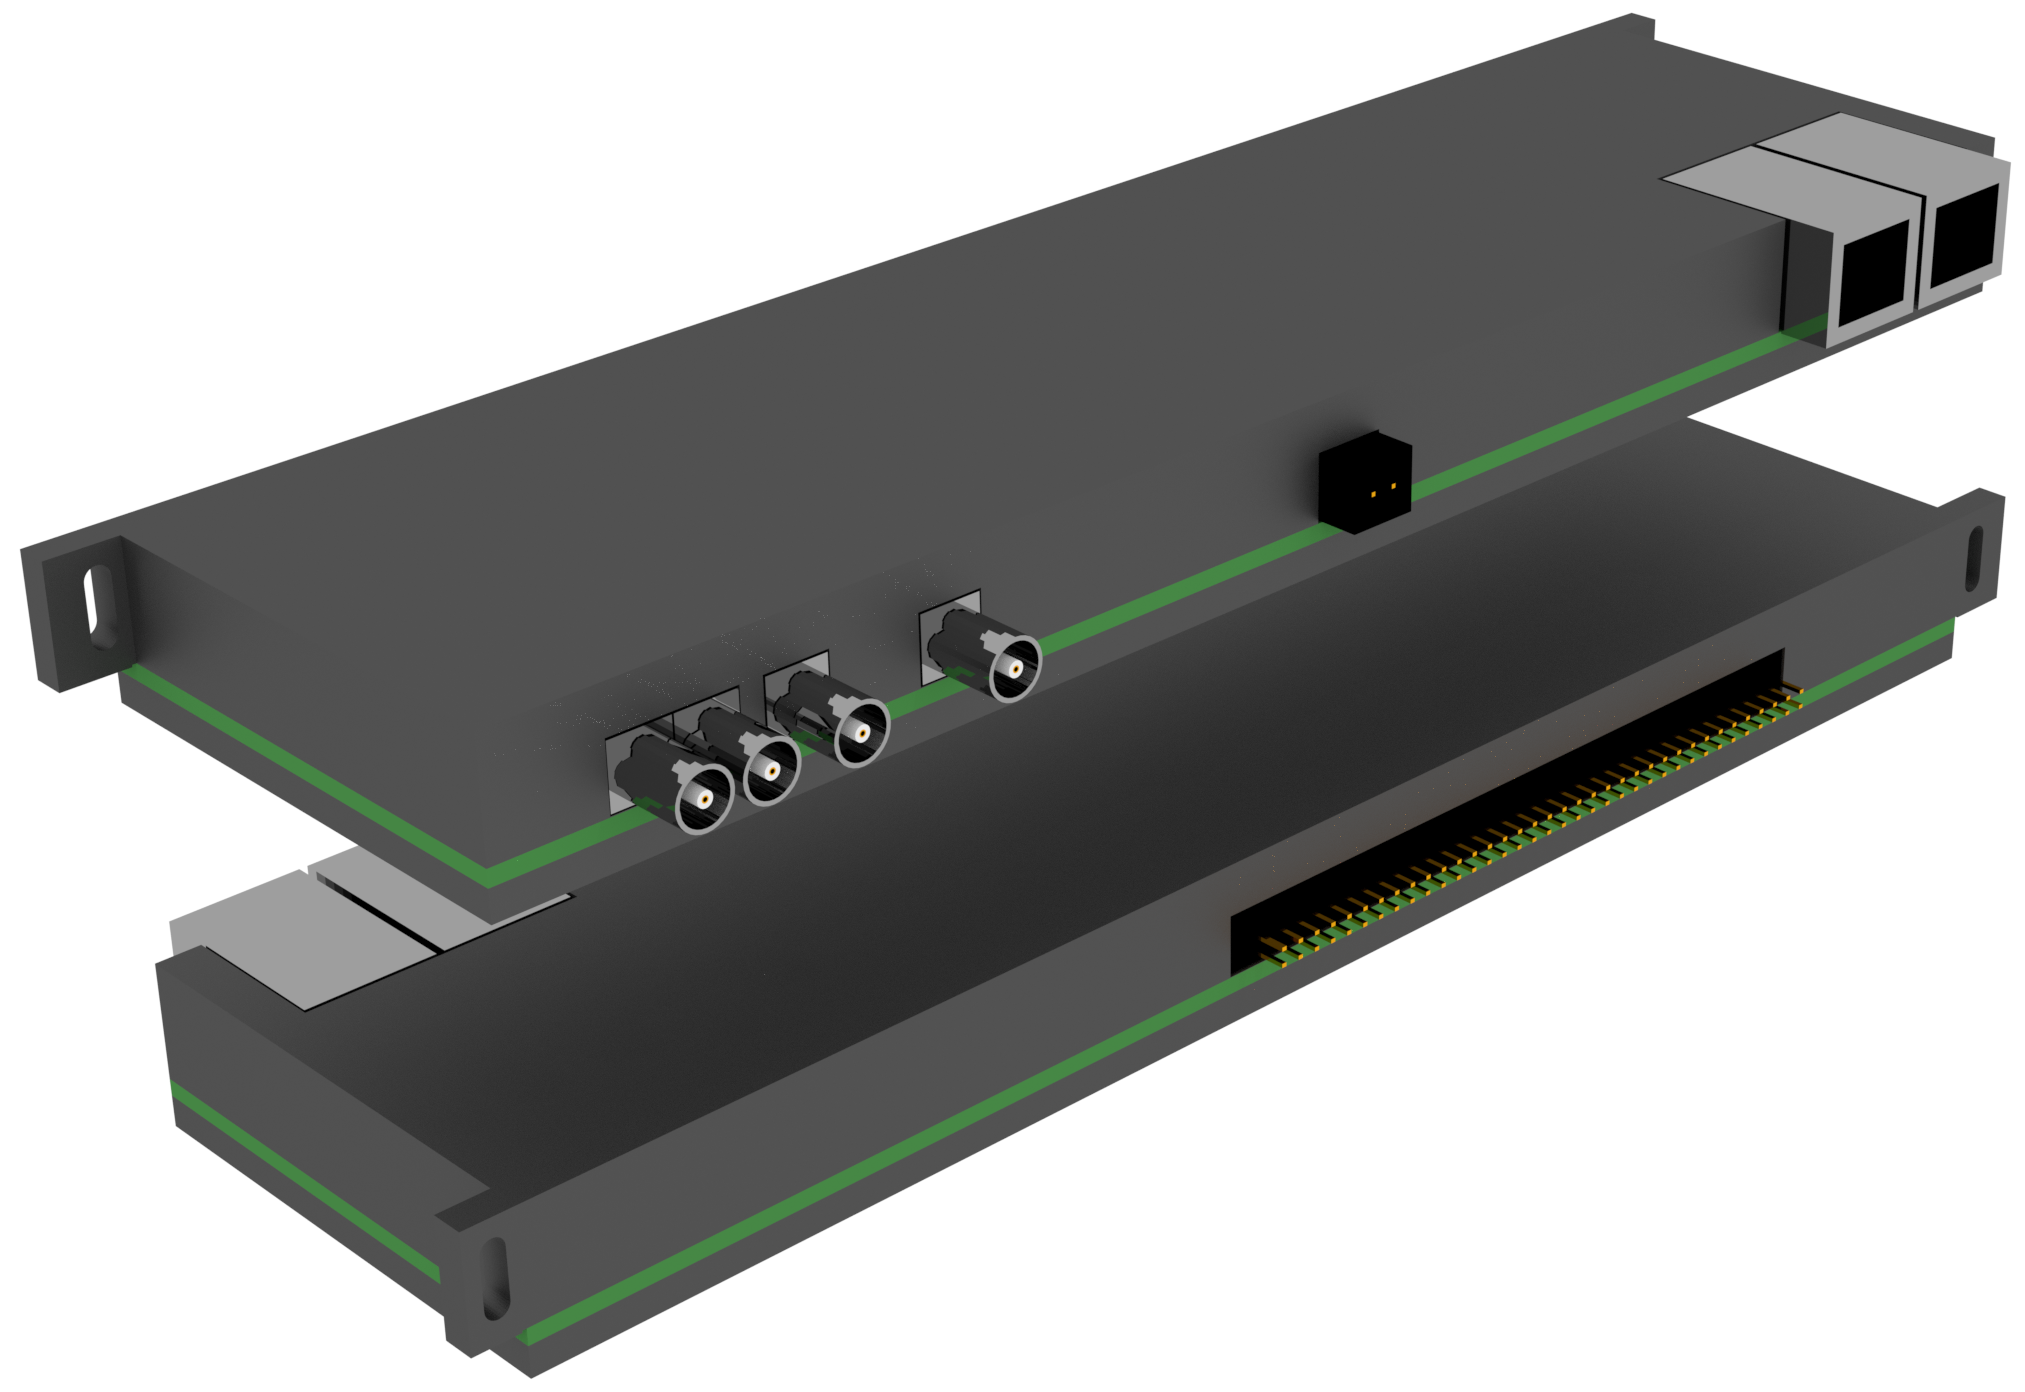
\includegraphics[width=\textwidth]{FEB}
  \caption{%
    This figure shows the ports of the \gls{feb} (top) and the connector for the \gls{crt} panel (bottom).
    The ports are (fltr): TIN, TOUT for external coincidence signals, T2, T1 for time reference signals, power connector, 2x fast ethernet.
    The electronic components' board is visible from outside (green).
  }
  \label{fig:feb}
\end{figure}

\subsection{Bias voltage generator}
Bias voltage is given by two opposed voltages: A stabilized power supply and the voltage output of a \gls{dac}.
The voltage of the power supply is adjustable in a range from 50V to 90V by varying manually a trimmer resistor and is common for all 32 \glspl{sipm} served by the \gls{feb}.
Individual adjustments for every channel are made using the output the \gls{dac} supplied on board.
See figure \ref{fig:voltage_generator} for a simplified scheme of the electronic circuit.

\begin{figure}
  \centering
  \begin{circuitikz}
    \node[ground] (g1) at (0, -1) {};
    \node[ground] (g2) at (8, -1) {};
    
    \draw (0, -1) -- (0, 0) to[V=$V_\text{DAC}$] (2, 0) to[R, -*] (4, 0) to[D] (6, 0);
    \draw (8, -1) -- (8, 0) to[V=$V_\text{trimmed}$] (6, 0);
    \draw (4, 0) to[short, -o] (4, -2);
    \draw (4, -2) node[right] {$S_i$};
  \end{circuitikz}
  \caption{%
    The bias voltage is generated using a voltage source trimmed by a resistor.
    Voltage fine tuning for every channel is made with a configurable \gls{dac}'s output.
    The \gls{dac}'s constant output corresponds to a DC-offset of the signal lines, the \gls{dac}'s full range is from +0.5V to +4.5V.
    Since the \gls{dac}'s output is positive, increasing its value actually reduces the effective bias voltage for the \gls{sipm}.
    The \gls{sipm} is depicted as a single diode in this scheme for simplicity.
  }
  \label{fig:voltage_generator}
\end{figure}

\subsection{Triggering logic}
One of the \gls{feb}'s features is to trigger events only when both \glspl{sipm} of the same scintillating bar present simultaneously a sufficently high signal.
The signal $S_i$ -- for the $i$th \gls{sipm} -- is amplified a charge amplifier and shaped with a RC-CR-shaper.
If the shaped signal is greater than the set threshold, the output of the discriminator $T_i$ is positive.
This output is combined with the corresponding signal of the associated \gls{sipm}, generating the pair trigger signal $P_i$.
If one of the pairs trigger a signals is positive, the \gls{cpu} tarts digitazion of the event.
\marginnote{This coincidence requirement reduces the number of events caused by incident gamma radiation significantly.}
Amplification, shaping and discrimination is done by CITIROC ASIC and signal logic is processed by a SPARTAN-6 \gls{fpga}.
See figure \ref{fig:fast_shaper_discriminator} for an illustration of the electronic circuit.

\begin{figure}
  \centering
  \begin{circuitikz}

    \node[buffer]     (amp1)    at (0, 0) {};
    \node[coordinate] (c1)      at (2, 0) {};
    \node[coordinate] (c2)      at (4, 0) {};
    \node[coordinate] (c2t)     at (4, 1.5) {};
    \node[coordinate] (c2tt)    at (4, 3) {};
    \node[buffer]     (amp2)    at (5, 0) {};
    \node[coordinate] (c3b)     at (6, -1) {};
    \node[ground]     (ground)  at (6, -2.5) {};
    \node[coordinate] (c3)      at (6, 0) {};
    \node[coordinate] (c3t)     at (6, 1.5) {};
    \node[coordinate] (c3tt)    at (6, 3) {};

    \node[op amp, yscale=-1]  (amp) at (8, -0.5) {};
    \node[and port]   (and) at (12, -0.775) {};

    % Inputs
    \draw (-1, 0) node[left] {$S_{2i}$};
    \draw (-1, 0) to[short, o-] (amp1.in);

    % RC-CR shaper
    \draw (amp1.out) to[R] (c1) to[C, -*] (c2);
    \draw (c2) -- (c2t) to[R, *-*] (c3t) -- (c3);
    \draw (c2) -- (c2tt) to[C] (c3tt) to[short, -*] (c3);
    \draw (c2) -- (amp2.in);
    \draw (amp2.out) -- (amp.+);

    % Connections to discriminator
    \draw (ground) to[V=$V_\text{DAC}$] (c3b) -- (amp.-);

    % Connections to the and port
    \draw (amp.out) -- (and.in 1);
    \draw (and.out) to[short, -o] (and.out);

    % Labels
    \draw (and.out)  node[right] {$P_i$};
    \draw (and.in 2) node[left] {$T_{2i+1}$};
    \draw (and.in 2) to[short, o-] (and.in 2);
    \draw (and.in 1) node[above left] {$T_{2i}$};

  \end{circuitikz}
  \caption{%
    Scheme of the electronic circuit to generate the trigger signal for a pair $P_i$ from the signals of two \glspl{sipm} $S_{2i}$ and $S_{2i+1}$.
    The amplifier, shaper and discriminator to generate associated signal $T_{2i+1}$ are not displayed for simplicity.
  }
  \label{fig:fast_shaper_discriminator}
\end{figure}

\subsection{Analog signal readout and digitization}
The \gls{feb} starts signal readout when an event trigger signal is triggered.
In that case the signal of the \glspl{sipm} is amplified, shaped using a slow RC-CR shaper and stored in a sample-and-hold circuit.
The stored analog signals are then digitized one by one using a 12-bit \gls{adc} and an analog multiplexer, to switch between the signals to digitalize.
Figure \ref{fig:slow_shaper} illustrates the electronic circuit.

\begin{figure}
  \centering
  \begin{circuitikz}

    \node[buffer] (amp1) at (0, 0) {};
    \node[coordinate] (c1) at (2, 0) {};
    \node[coordinate] (c2) at (4, 0) {};
    \node[coordinate] (c2t) at (4, 1.5) {};
    \node[coordinate] (c2tt) at (4, 3) {};
    \node[buffer] (amp2) at (5, 0) {};
    \node[coordinate] (c3) at (6, 0) {};
    \node[coordinate] (c3t) at (6, 1.5) {};
    \node[coordinate] (c3tt) at (6, 3) {};

    % Inputs
    \draw (-1, 0) node[left] {$S_i$};
    \draw (-1, 0) to[short, o-] (amp1.in);

    % RC-CR shaper
    \draw (amp1.out) to[R] (c1) to[C, -*] (c2);
    \draw (c2) -- (c2t) to[R, *-*] (c3t) -- (c3);
    \draw (c2) -- (c2tt) to[C] (c3tt) to[short, -*] (c3);
    \draw (c2) -- (amp2.in);
    \draw (amp2.out) -- (c3) -- ($(amp2.out) + (1, 0)$);
    \draw ($(amp2.out) + (1, 0)$) node[above] {$I_i$};

    % Switch and ADC
    \draw ($(amp2.out) + (1, 0)$)
      to[generic, l=S\&H] ($(amp2.out) + (3, 0)$)
      to[ospst=MUX] ($(amp2.out) + (4, 0)$)
      to[generic, l=ADC, -o] ($(amp2.out) + (6, 0)$);

  \end{circuitikz}
  \caption{%
    A series of amplificators and RC-CR slow shapers are used to treat the diode's signal before beind stored in the hold circuit.
  }
  \label{fig:slow_shaper}
\end{figure}

\subsection{Event data structure \& storage}
When an event is striggered and as soon as the \gls{adc} process is completed for all 32 channels, the result is combined with the time stamp to a packet of the following structure:

\begin{minted}{c}
  typedef struct {
    uint32_t flags;
    uint32_t T1;
    uint32_t T2;
    uint16_t adc[32];
  } FEBEVT_t;
\end{minted}

These event packets are stored in the internal ring buffer.
Once the capacity of 1024 events is reached, new events will override present ones.
The number of overwritten events is passed in the flags of the event packet.

\subsection{The Front-End Board software}

\paragraph{febdrv} communicates with \gls{feb} and sends commands to it.
febdrv allows to switch bias, data adquisition and configure the \gls{feb}.
It also publishes statistics and stati of the connected \glspl{feb} and their observed event packets.

\paragraph{febctl} sends commands to the febdrv to start and stop \gls{daq} and switch the \gls{feb}'s bias voltage.

\paragraph{febconf} reads configurations from files and sends them to the febdrv to change the \gls{feb}'s settings.

\paragraph{febmon} displays current status of the \gls{feb} published by febdrv.



\clearpage
\pagebreak

\section{Calibration of a Cosmic Ray Tagger module}
While time resolution of the \gls{crt} can be calibrated without directly knowing the gain, calibrating the latter is critical for position resolution and efficiency of a \gls{crt} module.
Given a fixed threshold, the efficiency of a \gls{sipm} depends strongly on the gain.
This section introduces the distributions of the signals observed by the \gls{crt} module, the distribution's associated parameters, gain determination and calibration.

\subsection{The signal spectrum}

The event data obtained from febdrv is collected and the signal values are counted for every \gls{sipm}, leading to each \gls{sipm}'s spectrum and the pedestal.
The resulting distributions for the pedestal vary in dependence of the observed \gls{sipm}, therefore a sample spectrum is displayed in figure \ref{fig:cal_pedestal_spectrum}.

\begin{figure}
  \centering
  \begin{tikzpicture}
    \node (img) {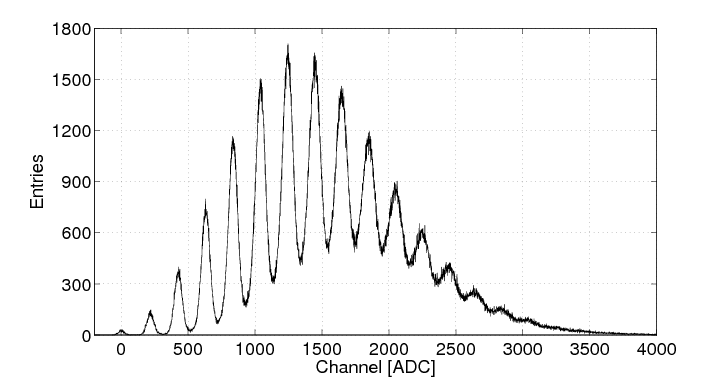
\includegraphics[width=\textwidth]{sipm_spectrum}};
    \node[label={[label distance=0.5cm,text depth=-1ex,rotate=90]above:pedestal}] at (-3, -1.5) {};
    \node[label={[label distance=0.5cm,text depth=-1ex,rotate=90]above:1 photo electron}] at (-2.6, -.5) {};
    \node[label={[label distance=0.5cm,text depth=-1ex,rotate=90]above:2 p.e.}] at (-2.2,-.8) {};
    \node[label={[label distance=0.5cm,text depth=-1ex,rotate=90]above:3 p.e.}] at (-1.8,0.2) {};
  \end{tikzpicture}
  \caption{%
    Sample spectrum of a \gls{sipm}.
    The first peak corresponds to the pedestal, followed by a series of peaks, each representing a number of simultaneously discharged cells.
    Since the uncertainties of the cells add up, the peaks get wider with increasing number of simultaneusly discharged cells.
  }
  \label{fig:cal_pedestal_spectrum}
\end{figure}

The spectrum of a \gls{sipm} consists of a series of peaks, the first peak corresponds to the pedestal, a gaussian distribution around the zero value.
The nature of this pedestal is the electronic noise and the current leaks generated by the electronic components.
The subsequent peaks correspond to simultaneously discharged \gls{sipm} cells and therefore to a number of photo electrons.
Since every peak corresponds to a number of simultaneously discharged cells, the distances between the position of the peaks corresponds to the gain of the \gls{sipm}.

\paragraph{Signal \& single photon resolution}
The signal in the readout is the sum of the signal when no avalanche occurrs -- also called pedestal -- and the avalanche signal
\begin{equation*}
	S_i = S_\text{pedestal} + i \cdot G,
\end{equation*}
where $G$ is the gain of signal in a \gls{sipm} and $i$ is the number of photo electrons or simultaneously discharged cells.

The fluctuations of the pedestal and gain uncertainties determine the single photon resolution:
\begin{equation*}
  \sigma(i)^2 = \sigma^2_\text{pedestal} + i \cdot \sigma^2_\text{gain},
\end{equation*}
where $i$ is the number of activated cells.
The fluctuations in the pedestal originate from unpredictable current leaks and readout electronics noise.
The uncertainties in the gains come from varying quenching resistances from cell to cell and the fluctuations during avalanche processes.

\paragraph{Dark rate, cross-talk \& after pulses} The dark rate is the event rate from avalanches generated by thermal or field mediated excitations of electrons in the silicon lattice and two correlated avalanche triggers: cross-talk and after pulses.

When the bias voltage is greater than the breakdown voltage, a charged carrier crossing the cell's p-n junction, can create a photon with sufficient energy to create an electron-hole pair.
The probability of this happening is of the order of $10^{-5}$, therefore for gains of the order of $10^5$, the number of these photons becomes significant\cite{1206.4154}.
It is important to point out, that these photons can propagate into nearby cells and initiate an avalanche.
This effect is called optical cross-talk.

During avalanches, electrons can be trapped in the Si-lattice and released later, producing a second avalanche after a characteristic time delay.
These avalanches are generally called after pulses.


\subsection{Determine the gain of a silicon photomultiplier}

Since the distance between neighboring peaks allows to compute the gain of the \glspl{sipm}, a method to identify the peaks, determine their positions and compute the distances is needed.
For this the part of the spectrum where the peaks are best visible is cut out.
\begin{figure}
  \centering
  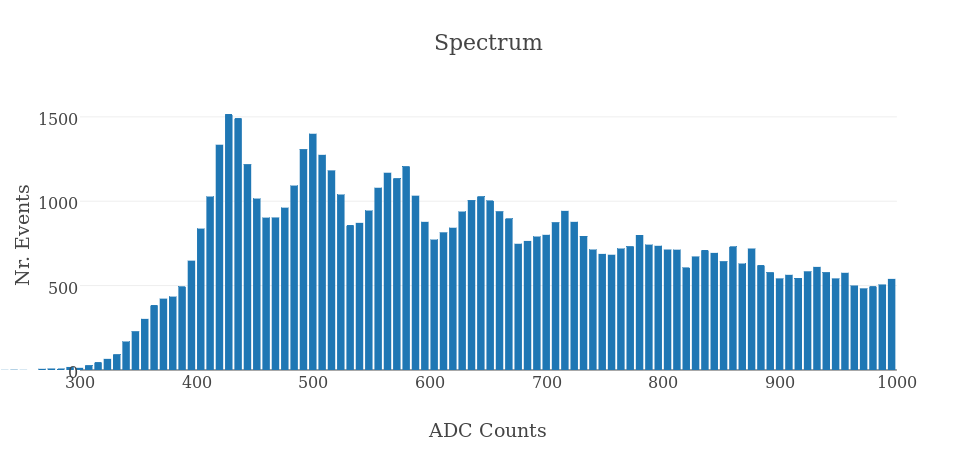
\includegraphics[width=\textwidth]{calibration/spectrum_cutout}
  \caption{%
    A small region of the spectrum has peaks, which are easy to identify.
  }
  \label{fig:spectrum_for_fit}
\end{figure}

First the positions of the peaks are estimated, using ROOT\cite{cern:root} and its TSpectrum class\cite{ROOT:TSpectrum}.
Three search parameters are used to find estimates: the width of the peaks, the bin size and the threshold.
Estimations are made by varying these parameters, each set of parameters leads to a search result with a number of peak candidates.

If the number of the estimated peak candidates is sufficently high, but doesn't exceed the number of expected peaks, a gaussian distribution is found to fit each peak candidate.
The resulting parameters are kept if the relative uncertainty of the position and the width is small\marginnote{$\sigma < 5\%$}.
Every set of search parameters leads therefore to a number of fitted peaks\marginnote{\ldots including fake peaks and missing some peaks sometimes!}.
The fitted positions are counted in a histogram, displayed in figure \ref{fig:cal_fitted_peaks}.

\begin{figure*}
  \centering
  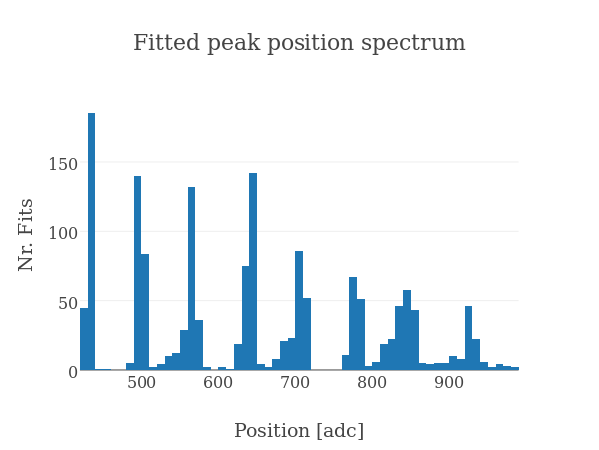
\includegraphics[width=.48\textwidth]{calibration/peak_spectrum}
  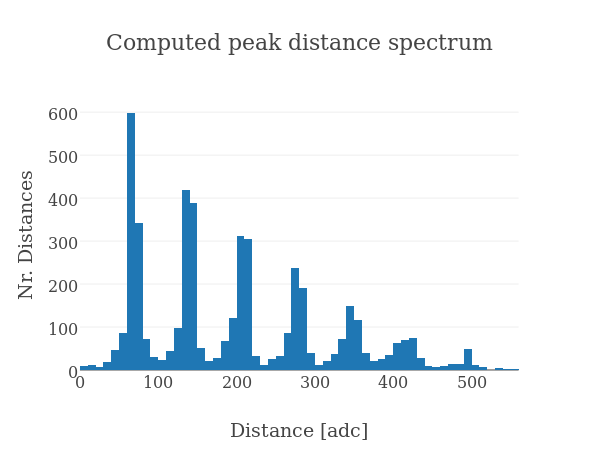
\includegraphics[width=.48\textwidth]{calibration/distances_spectrum}
  \caption{%
    The plot on the left shows the peak positions found for the given spectrum and different search parameters.
    The occurrences between the maxima show, that the search and fit method finds and registers fake peaks as well.
    The plot on the right displays the computed spectrum of distances.
    The first peak is the distance between two neigboring peaks.
    The second peak is the distance to the next proximate peaks, etc.
  }
  \label{fig:cal_fitted_peaks}
\end{figure*}

Since not only real peaks but fake peaks are identified and fitted as peaks, taking the mean and the standard deviation of the distances leads to undesired results.
This is avoided by computing the distances between the peaks for every set of fitted peaks.
Putting all these distances in a histogram -- as displayed in figure \ref{fig:cal_fitted_peaks} -- shows a series of clear features with decreasing height.
Assuming the number of found fake peaks is low, the most occurring distance is the distance between two neighboring peaks.
The position and width of a gaussian fitted around the greatest peak corresponds to the \gls{sipm}'s nominal gain and its uncertainty in \gls{adc} counts per photo electron -- see figure \ref{fig:cal_fitted_gain}.

\begin{figure}
  \centering
  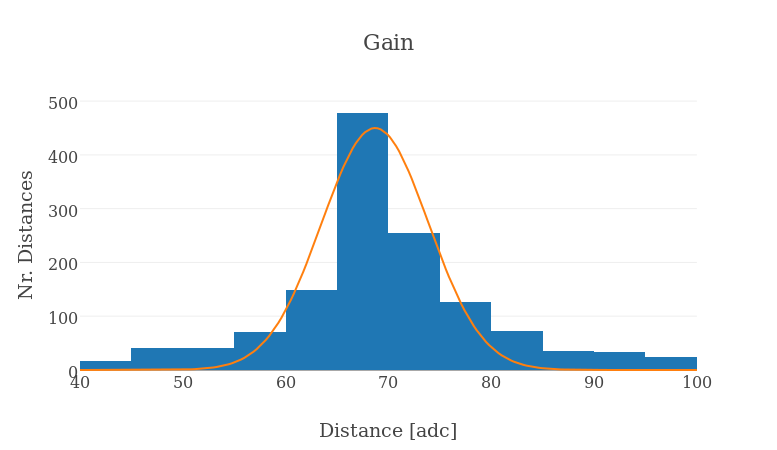
\includegraphics[width=\textwidth]{calibration/fitted_gain}
  \caption{%
    The plot displays the part of the histogram with the greatest peak and the fitted gaussian distribution around it.
  }
  \label{fig:cal_fitted_gain}
\end{figure}

\subsection{Dependency of the gain on the bias voltage}

When driven in Geiger mode, the cell of a \gls{sipm} behaves like a capacitance, accumulating charge -- which is responsible for the signal's gain -- due to a voltage supplied by the \gls{feb} charge
\begin{align}
  G &= \frac{C_\text{cell}}{e} (V_\text{bias} - V_\text{breakdown}) \label{eq:the_relation} \\
    &= \frac{C_\text{cell}}{e} V_\text{over voltage}  \\
    &\propto V_\text{over voltage},
\end{align}
where $C_\text{cell}$ is the capacitance of a cell, $e$ is the elementary electric charge,  $V_\text{breakdown}$ is the breakdown voltage of the \gls{sipm} and $V_\text{bias}$ is the bias voltage\marginnote{$V_\text{bias}$ is greater than $V_\text{breakdown}$ for \glspl{sipm} running in Geiger mode}.

This relation lets the observed spectrum and the gain depend heavily on the bias voltage.
A greater bias voltage leads to a greater charge stored in the \gls{sipm}'s cells and therefore to a greater discharge when the cell interacts with a photon.
This consequently leads to a higher gain.

The bias voltage of the \glspl{sipm} is generated by a manually trimmed stabilized power supply and a configurable \gls{dac} output voltage.
Since the trimmed output varies from \gls{feb} to \gls{feb} and the effective parameter used to calibrate the \glspl{crt} is the \gls{dac}'s setting, the gain is computed in dependence of the digital setting of the \gls{dac}.
The spectral change is displayed in figure \ref{fig:cal_changing_voltages}.

\begin{figure*}
  \centering
  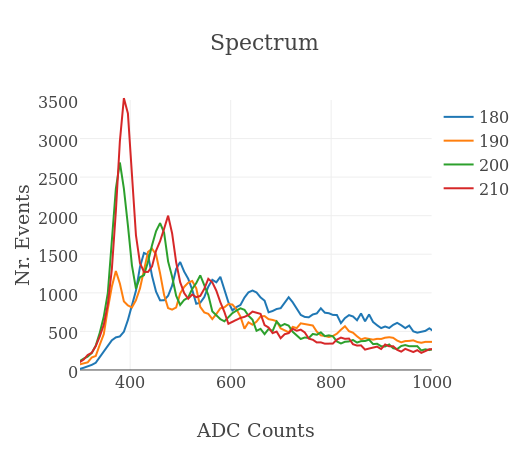
\includegraphics[width=.48\textwidth]{calibration/change_voltages}
  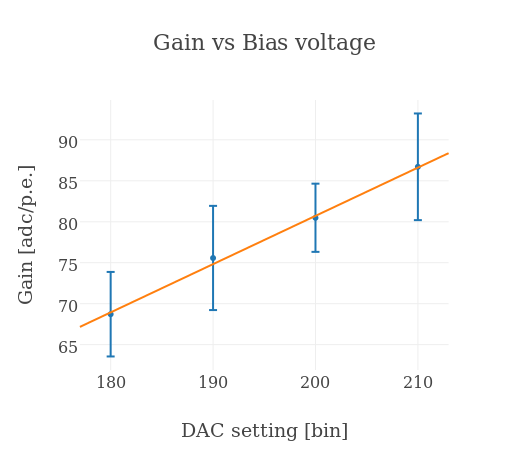
\includegraphics[width=.48\textwidth]{calibration/gain_vs_voltage}
  \caption{%
    The plot on the left displays spectra of a \gls{sipm} for increasing bias \gls{dac} output.
    It is clearly visible, that the spectrum shifts to the right with greater \gls{dac} setting.
    It is also visible, that the distance between the peaks increases with greater \gls{dac} setting.
    The plot on the right displays the dependence of the gain on the \gls{dac} setting.
  }
  \label{fig:cal_changing_voltages}
\end{figure*}

To determine this dependency, the bias voltage is changed by changing the setting responsible for the \gls{dac}'s output -- recall figure \ref{fig:voltage_generator}.
For every \gls{dac} setting, several sets of observations are made, the resulting relation is visible in figure \ref{fig:cal_changing_voltages}.
Even if the uncertainty of the gain is high at every observation point, a linear dependency can be guessed.

\subsection{The spectra of an uncalibrated panel vs. a calibrated panel}

The observed spectra vary from \gls{sipm} to \gls{sipm}.
For ideal components, fixing the bias voltage to a certain value for all \glspl{sipm} solves the problem.
In the case of real components a change in the spectrum is clearly visible, as displayed in figure \ref{fig:cal_uncalibrated_spectra}.

\begin{figure}
  \centering
  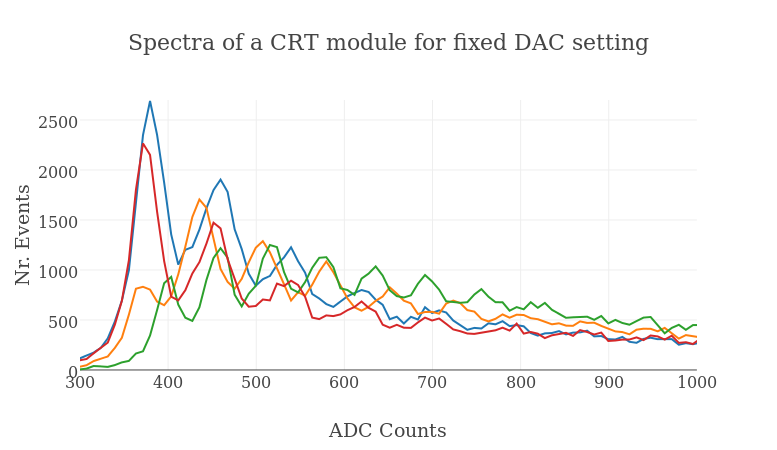
\includegraphics[width=\textwidth]{calibration/uncalibrated_spectra}
  \caption{%
    The spectra of 4 channels of the same \gls{crt} module are displayed.
    Every color represents one of the observed channels.
  }
  \label{fig:cal_uncalibrated_spectra}
\end{figure}

The gains of the \glspl{sipm} are computed and displayed in the left plot of figure \ref{fig:cal_vs_uncal} to visualize the distribution of gains in within a \gls{crt} module for fixed bias voltages.

With the aim to improve the spread of gains within a \gls{crt} module and improve therefore the uncertainty of the gain, the dependency of the gain on the bias voltage is computed for every \gls{sipm} of the \gls{crt} module.
The obtained curves are plotted in figure \ref{fig:cal_dependencies}.

\begin{figure}
  \centering
  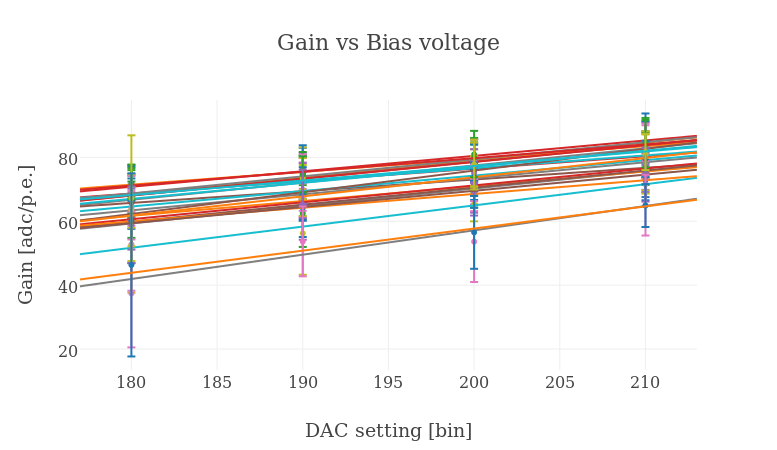
\includegraphics[width=\textwidth]{calibration/dependencies_run_1}
  \caption{%
    Change in gain in dependency of the \gls{dac} setting.
    Every colored line represents a different channel.
  }
  \label{fig:cal_dependencies}
\end{figure}

The inclination of the resulting slopes are similar for all the \glspl{sipm}.
The interval of configurable gains is narrow in within the given range of bias settings.
Due to the spread of the slope's position the interval of achievable gains for an uniform distribution is further reduced.

Using the computed dependencies and a simplified version of relation \ref{eq:the_relation}\marginnote{%
  $G = a \cdot \text{bias} + b \to \text{bias} = \frac{G-b}{a} $
} the settings for the biasing \gls{dac} is computed for every \gls{sipm}, with the aim to reduce the dispersion of gains within a module.

To test the sensitivity of the calibration, the bias settings are computed for three different gain within the attainable range: 75, 85 and 65 \gls{adc} counts per photo electron.
A set of observations is made for every set of computed settings and the gains are computed and counted for every \gls{sipm}.
The distributions are displayed in the right plot of figure \ref{fig:cal_vs_uncal}.

\begin{figure*}
  \centering
  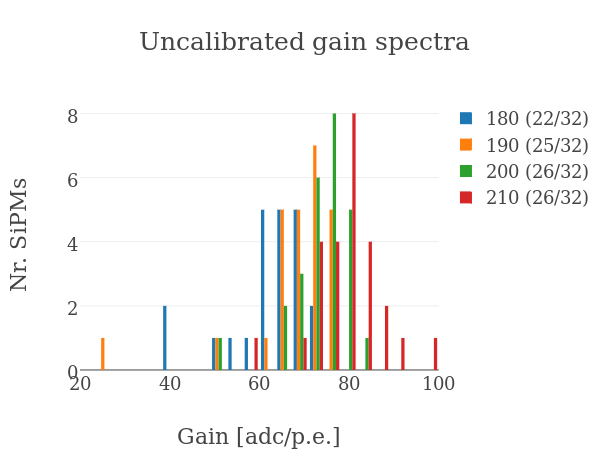
\includegraphics[width=.48\textwidth]{calibration/vorher}
  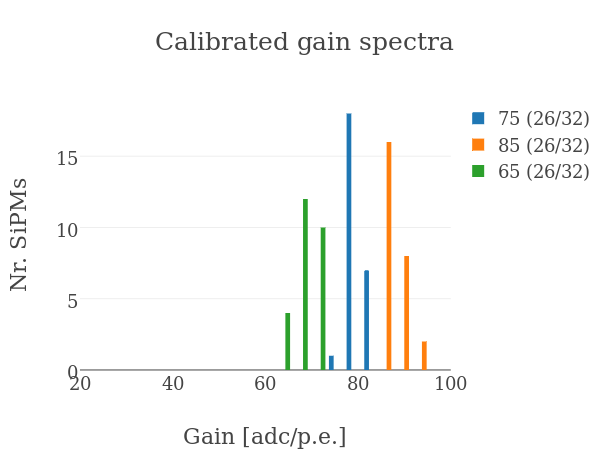
\includegraphics[width=.48\textwidth]{calibration/nacher}
  \caption{%
    The plot on the left shows the spectrum of computed gains for fixed \gls{dac} settings for every \gls{sipm}.
    The plot on the right displays the distribution of gains after the calibration process.
    To make the change more visible, the same range for the x axis is used.
  }
  \label{fig:cal_vs_uncal}
\end{figure*}

An important reduction of the spread of gains is observable in the plots of figure \ref{fig:cal_vs_uncal}.

For comparison with the uncalibrated spectra, the observed spectra for fixed nominal gains are displayed in figure \ref{fig:cal_vs_uncal_spectrum}.

\begin{figure*}
  \centering
  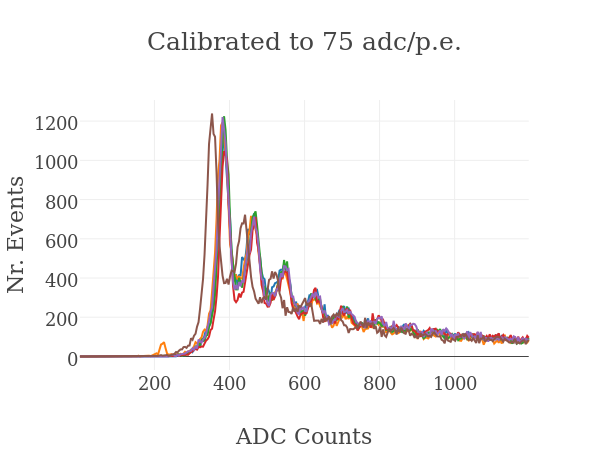
\includegraphics[width=.32\textwidth]{calibration/spectrum_75}
  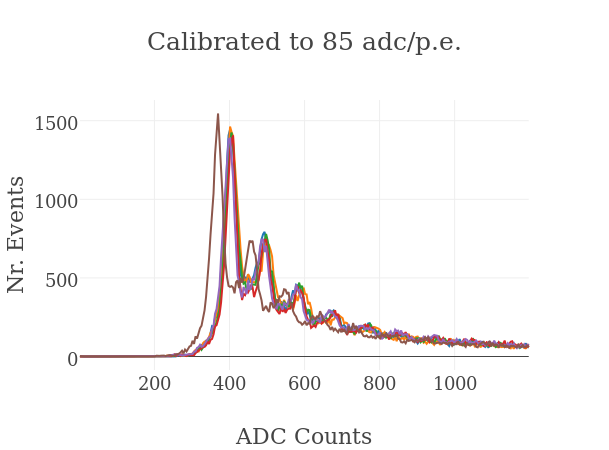
\includegraphics[width=.32\textwidth]{calibration/spectrum_85}
  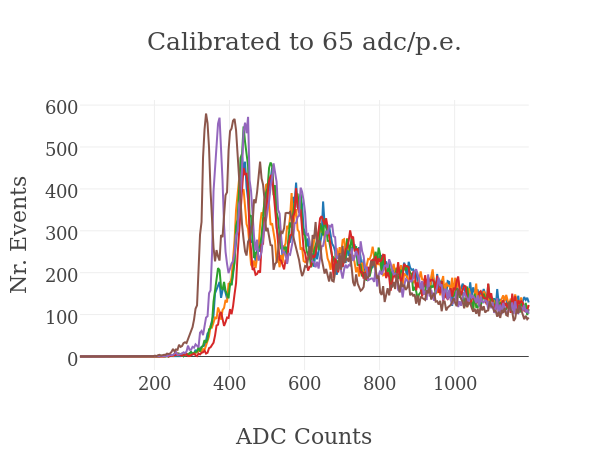
\includegraphics[width=.32\textwidth]{calibration/spectrum_65}
  \caption{%
    Observed spectra after calibration process.
  }
  \label{fig:cal_vs_uncal_spectrum}
\end{figure*}

An improvement in the spectra's uniformity in comparison to the uncalibrated spectra shown in figure \ref{fig:cal_uncalibrated_spectra} is visible.

\clearpage
\pagebreak

% Calibrating the panels
\section{Further studies on the Cosmic Ray Tracker}

Using the software bundled with the \gls{feb} and CalibRaTe, 3 further sets of observations are made to analyse the behaviour of the \gls{crt} modules, test the functionality of the data acquisition software and show the versatility of the evaluation tools.
This section lists the observations made with the \gls{crt} modules and analyzes part of the data of the observation sets.

\subsection{Sets of observations}

The \gls{feb}'s power supply voltage affects the generation of the bias voltage $V_\text{bias}$ and the output of the discriminator used to determine the threshold.
A change in the power supply voltage will changes the visible spectrum in the histograms.
Several sets of measurements have been taken using different power supply voltages to see this behavior and other effects.
The set of parameters for these observations are listed in table \ref{tab:os1}.

\begin{table}
  \centering
  \begin{tabular}{ c c c }
    Date       & \gls{feb} \& panels & Power supply voltage [V] \\
    \toprule
    2016-07-30
      & & \begin{tabular}{c c c c c}
        4.50 & 4.60 & 4.70 & \ldots & 5.10 \\
      \end{tabular}
    \\
    2016-08-03 & (71, 371) & 5.20   \\
    2016-08-04 &
      & \begin{tabular}{c c c}
        5.30 & 5.40 & 5.50 \\
      \end{tabular}
    \\
    \bottomrule
    \\
  \end{tabular}
  \caption{%
    Parameters of the observation set OS1.
    The \gls{feb} was powered with a Gw Instek GPS-4304 Power Supply, the power supply voltage's value was set manually and checked with a Fluke 115 Multimeter with an uncertainty of 0.01V.
    The power supply displayed a constant current at 0.52 (0.01) A.
  }
  \label{tab:os1}
\end{table}

The used data acquisition software was written to read data from several modules in parallel.
Another feature of the software is to permit the acquisition of data for a set of \gls{dac} settings without human interaction.
To test this functionality, the set of observations OS2 -- listed in table \ref{tab:os2} was made.

\begin{table}
  \centering
  \begin{tabular}{ c c c }
    Date       & \glspl{feb} \& panels & \gls{dac} setting [bin] \\
    \toprule
    2016-08-07
      & \begin{tabular}{ c c }
        (75, 375) & (76, 376) \\
        (77, 377) & (78, 378) \\
        (79, 379) & (80, 380) \\
      \end{tabular}
      & \begin{tabular}{ c c c c c }
         180 & 181 & 182 & \ldots & 200 \\
      \end{tabular}
    \\
    \bottomrule
    \\
  \end{tabular}
  \caption{%
    Parameters of the observation set OS2.
    The \gls{feb} was powered with rack power supply, the power supply voltage was kept constant at 4.63 (1) V and checked with a Fluke 115 Multimeter.
  }
  \label{tab:os2}
\end{table}

\subsection{Effects of changing power supply voltages on the pedestal}

A gaussian distribution is fitted around the pedestal of every \gls{sipm} for every parameter of observation set OS1.
The resulting positions, width and amplitudes are plotted in dependency of the power supply voltage in figure \ref{fig:pedestal_input}.

\begin{figure*}
  \centering
  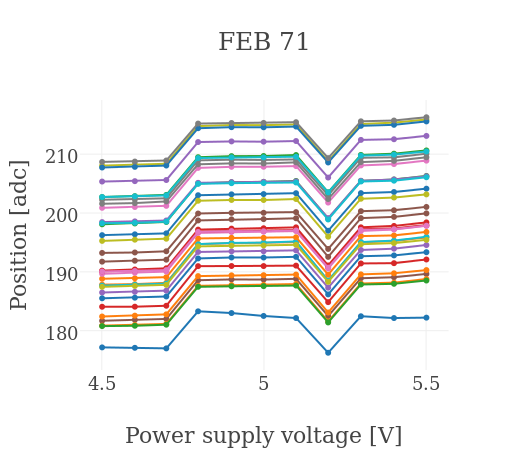
\includegraphics[width=.32\textwidth]{studies/input_voltages/pedestal_position_narrow}
  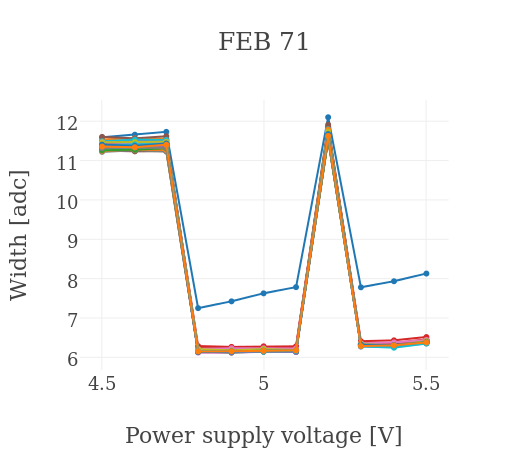
\includegraphics[width=.32\textwidth]{studies/input_voltages/pedestal_width_narrow}
  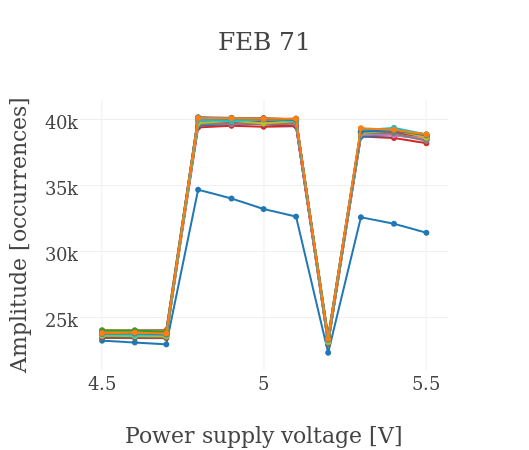
\includegraphics[width=.32\textwidth]{studies/input_voltages/pedestal_amplitude_narrow}
  \caption{
    Fitted pedestal positions for the 32 \glspl{sipm} of observation set OS1.
    Every colored line represents a \gls{sipm} of the \gls{crt} module.
    The uncertainties of the fits are tiny and not displayed in the plot.
  }
  \label{fig:pedestal_input}
\end{figure*}

The correlation of the signal of the 32 \glspl{sipm} is evident.
The plot also shows, that the pedestal of the \gls{crt} module has at least two diferent 'regimes'.
Notice the change of all three parameters at power supply voltages at and around 4.7V and 5.1V.
The pedestal changes by $\approx10\%$, while the width and amplitude change by a factor of 2.
The reason for this behaviour requires further study.

\subsection{Influences of the power supply voltage on the spectrum}

The behaviour of the spectrum is observed for changing power supply voltages, using the data from set OS1.
The spectrum of a \gls{sipm} is is displayed in dependency of the power supply voltage in figure \ref{fig:spectrum_input}.
\begin{figure}
  \centering
  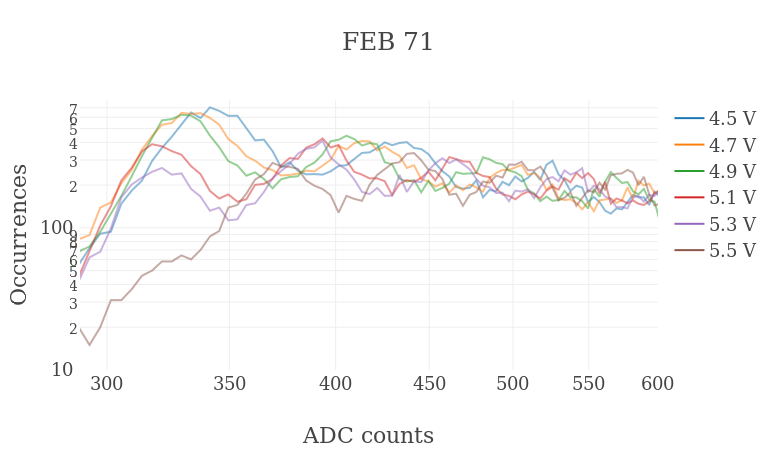
\includegraphics[width=\textwidth]{studies/input_voltages/spectrum_cutout}
  \caption{%
    Observed spectrum for changing power supply voltages.
    A shift of the spectrum to the left is clearly visible with increasing power supply voltage.
  }
  \label{fig:spectrum_input}
\end{figure}

The figure shows the spectrum of a \gls{sipm} for varying power supply voltages.
It is clearly visible, that the spectrum depends on the power supply voltage.
It is not obvious, though expected, that the distance between peaks change.
The shift of the spectrum to the left with raising voltage is undeniable.
This behavior shows the importance of a stable power supply voltage.

\subsection{Event rate vs. power supply voltages}

During \gls{daq} an important change of the time spent to acquire the same amount of data was noticed.
To study this behavior further, the \gls{feb}'s event rates were observed and stored using the output of the monitoring software febmon.
Since febmon does not specify which \gls{sipm} originates the observed event rate, spectra of the event rates are generated.
The event rate spectrum for every voltage is plotted histogram \ref{fig:eventrate_input}.

\begin{figure}
  \centering
  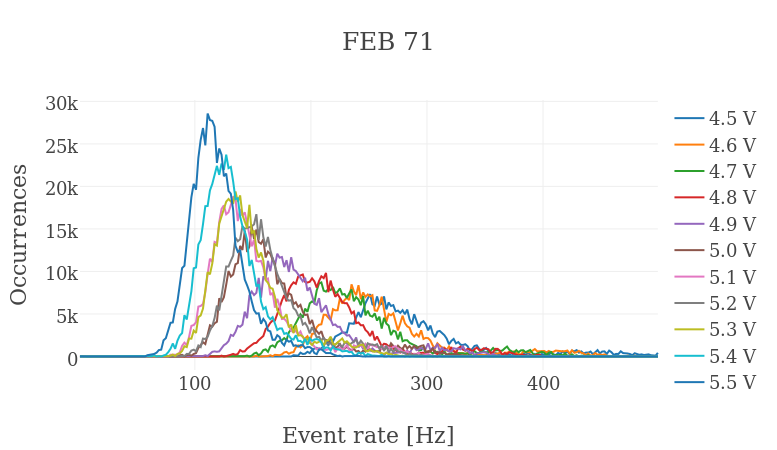
\includegraphics[width=\textwidth]{studies/input_voltages/event_rates}
  \caption{%
    Observed spectra of the event rates for \gls{feb} 71 and panel 371 for different power supply voltages.
    The shift to the left with increasing power supply voltage is evident.
  }
  \label{fig:eventrate_input}
\end{figure}

\pagebreak
The plot shows gaussian distributed spectra, whose shape and position depend cleary on the power supply voltage.
The distribution shifts to the left with increasing power supply voltage while getting thinner and gaining amplitude.

To see this effect more clearly, a gaussian distribution is fitted to each spectrum to determine its amplitude, position and width.
These fit parameters are plotted in dependence of the power supply voltage in figure \ref{fig:eventrate2_input} to see the dependency on the power supply voltage.

\begin{figure*}
  \centering
  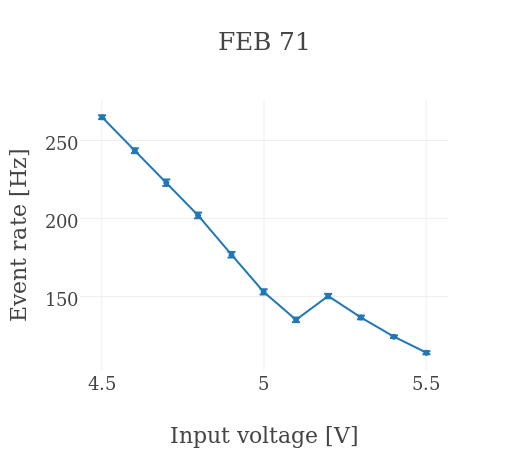
\includegraphics[width=.325\textwidth]{studies/input_voltages/eventrate_vs_voltage}
  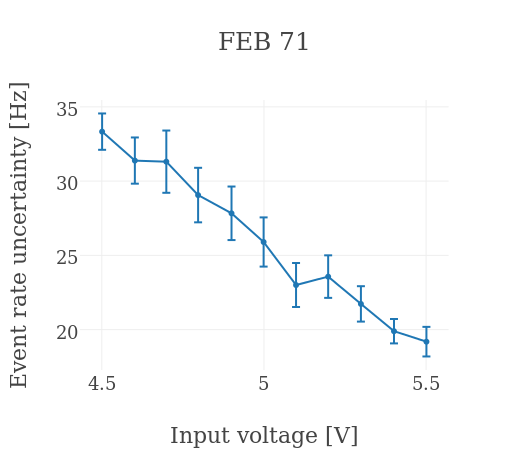
\includegraphics[width=.325\textwidth]{studies/input_voltages/eventrate_uncertainty_vs_voltage}
  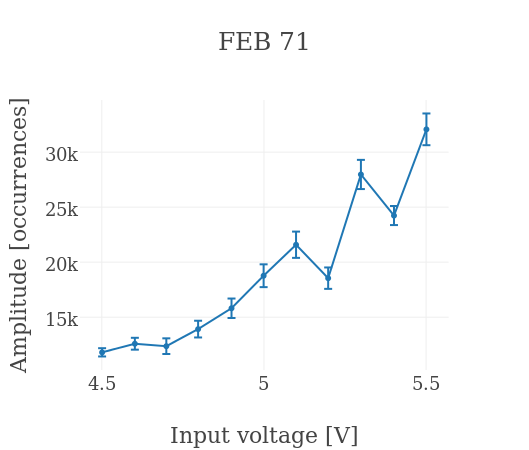
\includegraphics[width=.325\textwidth]{studies/input_voltages/eventrate_amplitude_vs_voltage}
  \caption{Fit parameters (fltr: position, width and amplitude) of the event rate distributions in dependency of the power supply voltages.}
  \label{fig:eventrate2_input}
\end{figure*}

The decrease of the event rate with increasing power supply voltage is obvious.
This decrease suggests a change in the detection efficiency.
The dispersion of the event rate spectra within a \gls{crt} module decreases with higher voltage, consequently the amplitude of the gaussians increases with higher power supply voltage.
Since the event rates decrease with higher voltage and each set of measurements contains the same amount of events, the time febmon observed the event rate increased.
Due to febmon's constant observation rate, the number of observations and therefore the amplitude of the spectra increases with longer observation time.

\subsection{Effects of changing bias voltages on the pedestal}

Since the pedestal is an indicator of the noise in the signal, studying its behavior in dependency of the bias voltage is of importance.
For this reason the pedestal is studied for the observation set OS2.
The positions and widths of the fitted gaussians are displayed in figures \ref{fig:pedestal_pos_bias} and \ref{fig:pedestal_wid_bias}.

\begin{figure}
  \centering
  \includegraphics[width=\textwidth]{studies/bias_voltages/pedestal_position_75}
  \caption{%
    Fitted pedestal positions in dependency of the bias voltage for one of the \gls{feb} of a observation set OS2.
    Every colored line represents a \gls{sipm} of the module.
  }
  \label{fig:pedestal_pos_bias}
\end{figure}

The plot displays a clear correlation of the pedestals change in position for all the \gls{sipm} signals.
This correlation indicates the independency of the \gls{sipm} on the change of position, suggesting the \gls{feb} as main contributor to this parameter.
This correlation is visible for all observed \gls{crt} panels.
The positions of the pedestals depend on the \gls{sipm}.
The spread of pedestal positions is assumed to be related to the spread of gains of an uncalibrated \gls{crt} module.

\begin{figure}
  \includegraphics[width=\textwidth]{studies/bias_voltages/pedestal_position_uncertainty_75}
  \caption{%
    Fitted pedestal widths in dependency of the bias voltage for one of the \gls{feb} of a observation set OS2.
    The widths of the pedestals are similar to each other, only one of the \glspl{sipm} has a wider pedestal.
    Every colored line represents a \gls{sipm} of the module.
  }
  \label{fig:pedestal_wid_bias}
\end{figure}

The width of the pedestal is similar for all the \glspl{sipm} of the same \gls{crt} module.
Only one \gls{sipm}'s pedestal is considerably wider than the rest.
This behavior is attributed to the greater difference in voltage during digitazing process for thefirst \gls{sipm} which leads to a greater uncertainty of the \gls{adc}'s input.
The width of the first \gls{sipm}'s pedestal tends to decrease with increasing bias voltage.

The computed positions and widths of the pedestal are counted for all the sets of OS2 and displayed in figure \ref{fig:pedestal_pos_spectra_bias}.

\begin{figure}
  \centering
  \includegraphics[width=\textwidth]{studies/bias_voltages/pedestal_position_spectra}
  \caption{
    The spectra of the fitted positions of the pedestal for the observation set OS2.
    Every color represents a different \gls{crt} module.
  }
  \label{fig:pedestal_pos_spectra_bias}
\end{figure}

The pedestals are distributed around a mean value which varies from \gls{crt} module to \gls{crt} module.
The distribution of the pedestals give an idea of the variation of the pedestal.

\begin{figure}
  \includegraphics[width=\textwidth]{studies/bias_voltages/pedestal_width_spectra}
  \caption{
    The spectra of the fitted widths of the pedestal for the observation set OS2.
    Each distribution contains the computed widths of all the \glspl{sipm} for all set bias voltages.
    Each color represents a different \gls{crt} module.
    A feature on the right of every distribution is visible, attributed to the first \gls{sipm} of every \gls{crt} module.
  }
  \label{fig:pedestal_wid_spectra_bias}
\end{figure}

The figure displays a variety of distributions, whose mean and standard deviation depends heavily on the observed \gls{crt} module.
The difference of the first \gls{sipm}'s pedestal width is visible in each distribution.

The change of position and width of the pedestal is observed in dependency of the bias voltage, by computing and counting all the changes of the respective parameters.
The resulting distributions are displayed in figure \ref{fig:pedestal_changes_bias}.

\begin{figure*}
  \centering
  \includegraphics[width=.48\textwidth]{studies/bias_voltages/change_pedestal_position}
  \includegraphics[width=.48\textwidth]{studies/bias_voltages/change_pedestal_width}
  \caption{%
    Histograms displaying the spectrum of changes in pedestal position, width and amplitude for observation set OS2.
  }
  \label{fig:pedestal_changes_bias}
\end{figure*}

The computed spectra of the parameters' differences are distributed around the origin.
The spectra of the pedestals' position is more spread than the spectra of the pedestals' width.

This study is done for a fixed power supply voltage.
Since the power supply voltage incluences the regime of the pedestal, a study including the variation of the power supply voltage and the bias voltage is recommended.

\clearpage
\newpage

% Calibrating the panels
\section{Conclusions}

The behavior of the amplitude spectrum obtained from several \gls{crt} modules under different bias voltages is studied and a method to determine a \gls{sipm}'s gain is developped.
The linear dependency of the gain on the bias voltage is been studied and used to elaborate a calibration method for the \gls{crt} modules.
The improvement of the calibrated amplitude spectrum is significant.

The calibration of the gain is a tidious task, with many influences of many parameters.
With the help of automated tools, human interaction can be reduced, making the calibration of the gain an affordable task.

The selection rules for the validity of the peaks in the fitting procedure can be improved to achieve smaller uncertainties.
Including the second and third most frequent distance between the peaks to reduce the gain's uncertainty needs to be studied.

The additional studies indicate an important dependency of the spectrum on the power supply voltage.
This effects need to be taken into consideration during and after \gls{crt} module calibration.

The study of the calibration results for varying power supply voltages is recommended.

The computed gains and bias settings of the calibration of the \gls{crt} module 75 is found in table \ref{tab:results}.


\begin{table*}
  \centering
  \begin{tabular}{ l c c c }
    Aimed gains &  75 & 85 & 65 \\
      & \begin{tabular}{c c c}
          \gls{sipm} & bias & gain \\
          \toprule
		0 & 192 & 77.5 (7.4) \\
		1 & 195 & 81.8 (2.6) \\
		2 & 192 & 81.3 (8.3) \\
		3 & 194 & 79.4 (5.2) \\
		4 & 196 & 80.5 (5.4) \\
		5 & 188 & 77.9 (7.0) \\
		6 & 189 & 79.6 (5.1) \\
		7 & 205 & 81.3 (6.4) \\
		8 & 207 & 77.8 (3.4) \\
		9 & 201 & 80.8 (5.1) \\
		10 & 209 & 79.8 (3.8) \\
		11 & 206 & 79.6 (3.1) \\
		12 & 207 & 78.8 (6.3) \\
		13 & 203 & 78.6 (3.0) \\
		15 & 215 & 76.4 (2.2) \\
		18 & 215 & 81.1 (3.6) \\
		19 & 193 & 78.9 (3.6) \\
		20 & 199 & 80.9 (3.2) \\
		21 & 192 & 79.6 (4.1) \\
		22 & 195 & 78.9 (4.8) \\
		23 & 202 & 81.0 (5.6) \\
		24 & 189 & 79.8 (5.5) \\
		25 & 210 & 81.0 (6.5) \\
		26 & 230 & 81.6 (3.9) \\
		27 & 198 & 79.3 (3.6) \\
		30 & 217 & 78.2 (4.0) \\
          \bottomrule
        \\
        \end{tabular}
      & \begin{tabular}{c c c}
          \gls{sipm} & bias & gain \\
          \toprule
		0 & 209 & 87.9 (5.7) \\
		1 & 219 & 91.8 (6.2) \\
		2 & 211 & 89.8 (5.9) \\
		3 & 212 & 88.3 (4.5) \\
		4 & 221 & 92.8 (5.4) \\
		5 & 212 & 88.3 (5.7) \\
		6 & 208 & 87.9 (5.5) \\
		7 & 233 & 95.0 (5.2) \\
		8 & 227 & 86.4 (3.6) \\
		9 & 222 & 88.9 (5.8) \\
		10 & 231 & 89.3 (3.6) \\
		11 & 225 & 87.1 (7.3) \\
		12 & 226 & 88.7 (4.4) \\
		13 & 223 & 88.4 (7.4) \\
		15 & 234 & 85.8 (2.5) \\
		18 & 237 & 88.4 (3.7) \\
		19 & 211 & 88.0 (3.2) \\
		20 & 214 & 88.1 (3.6) \\
		21 & 210 & 88.3 (4.7) \\
		22 & 214 & 85.5 (4.2) \\
		23 & 218 & 87.5 (7.9) \\
		24 & 212 & 89.7 (4.4) \\
		25 & 230 & 89.6 (4.1) \\
		26 & 249 & 89.8 (4.4) \\
		27 & 214 & 87.8 (6.6) \\
		30 & 235 & 87.6 (2.2) \\
          \bottomrule
        \\
        \end{tabular}
      & \begin{tabular}{c c c}
          \gls{sipm} & bias & gain \\
          \toprule
		0 & 174 & 70.6 (3.2) \\
		1 & 172 & 67.5 (7.3) \\
		2 & 173 & 68.2 (6.2) \\
		3 & 176 & 69.8 (5.7) \\
		4 & 171 & 65.6 (7.1) \\
		5 & 164 & 65.8 (6.4) \\
		6 & 169 & 65.0 (12.1) \\
		7 & 177 & 67.8 (12.4) \\
		8 & 188 & 68.8 (2.1) \\
		9 & 181 & 72.1 (6.4) \\
		10 & 186 & 64.3 (8.0) \\
		11 & 188 & 71.1 (3.6) \\
		12 & 188 & 69.4 (3.3) \\
		13 & 183 & 69.5 (2.6) \\
		15 & 196 & 67.6 (2.6) \\
		18 & 192 & 69.1 (4.2) \\
		19 & 175 & 69.8 (3.2) \\
		20 & 184 & 73.0 (2.8) \\
		21 & 173 & 68.5 (8.8) \\
		22 & 176 & 67.0 (6.9) \\
		23 & 186 & 71.4 (4.7) \\
		24 & 167 & 65.0 (10.7) \\
		25 & 190 & 71.1 (2.5) \\
		26 & 212 & 72.4 (8.3) \\
		27 & 181 & 71.6 (7.3) \\
		30 & 198 & 67.0 (5.5) \\
          \bottomrule
        \\
        \end{tabular}
    \\
  \end{tabular}
  \\
  \caption{%
    Results of the calibration of \gls{crt} module 75 for a power supply voltage of 5.5 (0.1) V.
    The resulting settings for the bias changing \gls{dac} and corresponding computed gains are listed for the three aimed gains.
    The gain is given in \gls{adc} counts per photo-electron.
  }
  \label{tab:results}
\end{table*}


\clearpage
\newpage

%% Code poentry
\section{CalibRaTe - A calibration software bundle for the Cosmic Ray Tracker}
The goal of the CalibRaTe is to provide the required tools to run calibration studies on the \gls{crt}.
CalibRaTe consists of several components written in Python, C and C++ capable to communicate through ZeroMQ sockets.
This section aims to introduce the used technologies and lists the components of CalibRaTe showing at the same time their functionality and usage.

\subsection{Message queues - ZeroMQ in a nutshell}

Message queues allow to write several small programs (task processors) which run independently and communicate through sockets.
When programming message queues, every task can be solved by a custom component, permitting a fast and agile development.
One component publishes events, another aggregates them to histograms, a third computes gain and pedestal, a forth stores the results in a database, \ldots
And if one of the components tends to overload, several instances of it can be started and run in parallel to balance out the workload.

The message queue library used to handle the communication between the components of CalibRaTe is ZeroMQ, since it is fast, reliable and available for most modern programming languages like C, C++ and python.\marginnote{Ian Barber introduces ZeroMQ in his \href{https://www.youtube.com/watch?v=v6AGUeZOVSU}{talk \emph{ZeroMQ is the answer} at the PHP UK Conference 2011}}
ZeroMQ provides the following types of communication sockets:

\paragraph{Request \& response} sockets enforce a two way communication between a pair processes.
In general every request needs a response before a new request can be sent.
The process receiving the messages is blocked until a message arrives.
This behaviour can be altered using an optional flag.

\paragraph{Publish \& subscribe} sockets allow a publishing process to send equivalent messages to many subscribing processes.
The subscribers can use filters to subscribe to specific types of messages.

\paragraph{Push \& pull} is a one way communication socket, meaning that pullers cannot send messages to the pusher.
The pusher can push messages independent of the status of the last pushed message.
Every pushed message is handled by exactly one puller.

\subsection{The components}

\paragraph{histos} is an histogram builder for structures of type febevt.
The histogram builder requires the serial number of the \gls{feb} to which it is assigned and a configuration to configure the \gls{feb}.
The configuration can be given either as a path to a configuration file or as a hexadecimal string.
Histos includes a help option to display the available program options:

\begin{minted}{text}
 #> histos --help
 Usage: histos [OPTION...] [VCH0 [VCH1 VCH2 ... VCH31]]
 Histos -- a histogram builder for the feb driver

   -A, --all                  Enable all channels
   -B, --as_is                Take power amplification from config file
   -c, --config=FILE          Read configuration from FILE
   -C, --continuous           Run continuously
   -d, --driver=DRIVER        Driver,      Ex. tcp://localhost:5555
   -D, --debug                Produce debug output
   -f, --febsn=SERIAL         The SERIAL number of the frontend board
   -i, --input=INPUT          Data source, Ex. tcp://localhost:5556
   -n, --events=EVENTS        Number of EVENTS to collect
   -o, --output=OUTPUT        Data sink,   Ex. tcp://localhost:6000
   -v, --verbose              Produce verbose output
   -x, --hexstring=HEX        Read configuration from HEX
   -?, --help                 Give this help list
       --usage                Give a short usage message
   -V, --version              Print program version

 Mandatory or optional arguments to long options are also mandatory or optional
 for any corresponding short options.

 Report bugs to <pablo.verges@lhep.unibe.ch>.
\end{minted}

When a histos instance is started, it will load the given configuration into memory, connect to febdrv and start building histograms with the number of events given as program option.
Histos has 3 main running modes: 'as is', 'all' and the normal running mode.

If the option 'as is' is activated, data adquisition will run without changing any parameter of the configuration passed as argument option.
Using the option 'all' will activate power amplification for all the \glspl{sipm}.
When running histos in normal mode, power amplification is only activated for a pair of \glspl{sipm} at the time.
The logic for the normal run mode is displayed in figure \ref{fig:histos_logic}.

\begin{figure}
  \centering
  \pgfdeclarelayer{marx}
  \pgfsetlayers{main,marx}
  \providecommand{\cmark}[2][]{%
    \begin{pgfonlayer}{marx}
      \node [nmark] at (c#2#1) {#2};
    \end{pgfonlayer}{marx}
    }
  \providecommand{\cmark}[2][]{\relax} 
  \begin{tikzpicture}[%
      >=triangle 60,              % Nice arrows; your taste may be different
      start chain=going below,    % General flow is top-to-bottom
      node distance=6mm and 37mm, % Global setup of box spacing
      every join/.style={norm},   % Default linetype for connecting boxes
      ]
  \tikzset{
    base/.style={draw, on chain, on grid, align=center, minimum height=4ex},
    proc/.style={base, rectangle, text width=7.5em},
    test/.style={base, diamond, aspect=2, text width=5em},
    coord/.style={coordinate, on chain, on grid, node distance=6mm and 25mm},
    norm/.style={->, draw},
    it/.style={font={\small\itshape}}
  }
  \node [proc]               (p0) {initialize environment};
  \node [proc, join]         (n1) {loop over pairs};
  \node [proc, join]              {set trigger on pair};
  \node [proc, join]         (p5) {start data acquisition};
  \node [proc, join]         (p2) {receive event list};
  \node [proc, join]         (n9) {loop over events};
  \node [proc, join]         (p1) {parse event};
  \node [test, join]         (t1) {last event?};
  \node [test]               (t2) {enough?};
  \node [proc]               (p3) {stop data acquisition};
  \node [test, join]         (t3) {last pair?};
  \node [proc]               (p6) {send histograms};
  \node [proc, join]              {close environment};
  \node [coord, right=of t3] (c1) {};
  \node [coord, right=of t2] (c3) {};
  \node [coord, right=of p2] (c4) {};
  \node [coord, right=of t1] (c5) {};
  \node [coord, right=of n9] (c6) {};

  \node [coord, right=of n1] (n2) {};

  % 
  \node [proc, densely dashed, left=of p5, it] (p7)  {config};
  \node [proc, densely dashed, left=of p2, it] (p8)  {data source};
  \node [proc, densely dashed, left=of p3, it] (p9)  {config};
  \node [proc, densely dashed, left=of p6, it] (p10) {data sink};

  % External connections
  \draw [densely dashed] (p7) -- (p5);
  \draw [densely dashed] (p8) -- (p2);
  \draw [densely dashed] (p3) -- (p9);
  \draw [densely dashed] (p10) -- (p6);

  \path (t1) to node [near start, xshift=1em] {$y$} (t2);
  \draw [*->,solarized-blue] (t1) -- (t2);
  \path (t2) to node [near start, xshift=1em] {$y$} (p3);
  \draw [*->,solarized-blue] (t2) -- (p3);
  \path (t3) to node [near start, xshift=1em] {$y$} (p6);
  \draw [*->,solarized-blue] (t3) -- (p6);
  \path (t3) to node [near start, yshift=1em] {$n$} (c1);
  \draw [o->,solarized-red] (t3) -- ($(c1) + (3em, 0)$) -- ($(n2) + (3em, 0)$) -- (n1);
  \path (t2) to node [near start, yshift=1em] {$n$} (c3);
  \draw [o->,solarized-red] (t2) -- ($(c3) + (1.5em,0)$) -- ($(c4) + (1.5em,0)$) -- (p2);
  \path (t1) to node [near start, yshift=1em] {$n$} (c5);
  \draw [o->,solarized-red] (t1) -- (c5) -- (c6) -- (n9);

  \end{tikzpicture}
  \caption{%
    Schematic representation of the logic implemented in the histogram builder
    \emph{config}, \emph{data source} and \emph{data sink} are ressources available through ZeroMQ.
    If run in \emph{server} mode, the histogram builder will restart looping over the pairs after sending the histograms.
    The data received from the data source is a buffer of FEB events.
    The data sent to the sink is a struct with histograms for pedestal and spectrum for every channel of the FEB.
  }
  \label{fig:histos_logic}
\end{figure}

When a histos instance has collected enough data, it will push the resulting histograms for the pedestal and the spectra in a c structure, containing as well the configuration used for the run and the serial number of the \gls{feb} (the 5th byte of its mac address).
\begin{minted}{c}
  typedef struct {
    uint8_t  mac5;
    uint8_t  sc[143];
    uint32_t pedestal[32][4096];
    uint16_t spectrum[32][4096];
  } HISTOGRAMS_t;
\end{minted}
If histos is run with the continuous option, the histograms are emptied and data adquisition is restarted, else the histos instance disconnects and exits.

\paragraph{fitter} is a peak fitter and distance computing software for histograms.
Fitter needs a tcp socket to read tasks from and a tcp socket to push the computed results to.
The incoming histograms need to be json encoded and provide a key for task identification.
Read out of histograms from ROOT-files is planned but not yet implemented.

\begin{minted}{text}
 #> fitter --help
 Allowed options:
   -h [ --help ]              produce help message
   -i [ --input ] arg         Input socket.  Ex. tcp://localhost:7000
   -o [ --output ] arg        Output socket. Ex. tcp://localhost:8000

\end{minted}

\subsection{seqdaq}
\subsection{condaq}
\subsection{progdaq}

\subsection{The calibration message queue}

TODO: set the right voltage setting automatically
Determine the gain for a list of given voltages estimate the

\begin{figure}
  \centering
  \pgfdeclarelayer{marx}
  \pgfsetlayers{main,marx}
  \providecommand{\cmark}[2][]{%
    \begin{pgfonlayer}{marx}
      \node [nmark] at (c#2#1) {#2};
    \end{pgfonlayer}{marx}
    }
  \providecommand{\cmark}[2][]{\relax} 
  \begin{tikzpicture}[%
      >=triangle 60,               % Nice arrows; your taste may be different
      start chain=going below,     % General flow is top to bottom
      node distance=16mm and 40mm, % Global setup of box spacing
      every join/.style={norm},    % Default linetype for connecting boxes
      ]
  \tikzset{
    base/.style={draw, on chain, on grid, align=center, minimum height=4ex},
    proc/.style={base, rectangle, text width=4.5em},
    test/.style={base, diamond, aspect=2, text width=5em},
    coord/.style={coordinate, on chain, on grid},
    nmark/.style={draw, cyan, circle, font={\sffamily\bfseries}},
    norm/.style={->, draw},
    free/.style={->, draw, solarized-green},
    cong/.style={->, draw, solarized-red},
  }

  % Define the processes in the middle
  \node [proc]                (h1)  {histos};
  \node [proc]                (f1)  {fitter};
  \node [proc]                (h2)  {histos};
  \node [proc]                (m1)  {calibrator};
  \node [proc]                (h3)  {histos};
  \node [proc]                (f2)  {fitter};
  \node [proc]                (h4)  {histos};

  % Caption
  \node [coord]             (l) {};
  \node [coord, left=of l]  (ll) {};
  \node [coord, right=of l] (lr) {};

  % Define the processes to the left
  \node [coord, left=of h1]   (cl1) {};
  \node [coord, left=of f1]   (cl2) {};
  \node [coord, left=of h2]   (cl3) {};
  \node [proc, left=of m1]    (d1)  {driver};
  \node [coord, left=of h3]   (cl4) {};
  \node [coord, left=of f2]   (cl5) {};
  \node [coord, left=of h4]   (cl6) {};

  % Define the processes to the right
  \node [coord, right=of h1]   (cr1) {};
  \node [coord, right=of f1]   (cr2) {};
  \node [coord, right=of h2]   (cr3) {};
  \node [proc,  right=of m1]   (a1)  {archiver};
  \node [coord, right=of h3]   (cr4) {};
  \node [coord, right=of f2]   (cr5) {};
  \node [coord, right=of h4]   (cr6) {};

  % Request / Response
  \draw [<->,densely dotted] (m1) -- (d1);
  \draw [<->,densely dotted] ($(d1.north) + ( 0.5em,0)$)  -- ($(cl1) + ( 0.5em,-0.5em)$) -- ($(h1.west) + (0,-0.5em)$);
  \draw [ ->,densely dotted]                                 ($(cl3) + ( 0.5em,-0.5em)$) -- ($(h2.west) + (0,-0.5em)$);
  \draw [ ->,densely dotted]                                 ($(cl4) + ( 0.5em, 0.5em)$) -- ($(h3.west) + (0, 0.5em)$);
  \draw [<->,densely dotted] ($(d1.south) + ( 0.5em,0)$)  -- ($(cl6) + ( 0.5em, 0.5em)$) -- ($(h4.west) + (0, 0.5em)$);

  % Publish / Subscribe
  \draw [ ->,densely dashed] ($(d1.north) + (-0.5em,0)$)  -- ($(cl1) + (-0.5em, 0.5em)$) -- ($(h1.west) + (0, 0.5em)$);
  \draw [ ->,densely dashed]                                 ($(cl3) + (-0.5em, 0.5em)$) -- ($(h2.west) + (0, 0.5em)$);
  \draw [ ->,densely dashed]                                 ($(cl4) + (-0.5em,-0.5em)$) -- ($(h3.west) + (0,-0.5em)$);
  \draw [ ->,densely dashed] ($(d1.south) + (-0.5em,0)$)  -- ($(cl6) + (-0.5em,-0.5em)$) -- ($(h4.west) + (0,-0.5em)$);

  % Push / Pull
  \draw [ ->] (h1) -- (f1);
  \draw [ ->] (h2) -- (f1);
  \draw [ ->] (h1) -- (cr1) -- (a1);
  \draw [   ] (h2) -- (cr3);
  \draw [   ] (h3) -- (cr4);
  \draw [ ->] (h4) -- (cr6) -- (a1);
  \draw [ ->] (h3) -- (f2);
  \draw [ ->] (h4) -- (f2);
  \draw []    (f1) -- (cr2);
  \draw []    (f2) -- (cr5);
  \draw [ ->] (a1) -- (m1);

  % Caption
  \draw [<->,densely dotted] ($(ll) + (-2em,0)$)
    -- node[yshift=-3em]{REQ/REP}
    ($(ll) + (2em, 0)$);
  \draw [->,densely dashed] ($(l)  + (-2em,0)$)
    -- node[yshift=-3em]{PUB/SUB}
    ($(l)  + (2em, 0)$);
  \draw [->]                ($(lr) + (-2em,0)$)
    -- node[yshift=-3em]{PUSH/PULL}
    ($(lr) + (2em, 0)$);

  \end{tikzpicture}
  \caption{%
    Architecture of the calibration message queue implementation
  }
  \label{fig:architecture}
\end{figure}


\begin{figure}
  \centering
  \pgfdeclarelayer{marx}
  \pgfsetlayers{main,marx}
  \providecommand{\cmark}[2][]{%
    \begin{pgfonlayer}{marx}
      \node [nmark] at (c#2#1) {#2};
    \end{pgfonlayer}{marx}
    }
  \providecommand{\cmark}[2][]{\relax} 
  \begin{tikzpicture}[%
      >=triangle 60,              % Nice arrows; your taste may be different
      start chain=going below,    % General flow is top-to-bottom
      node distance=6mm and 37mm, % Global setup of box spacing
      every join/.style={norm},   % Default linetype for connecting boxes
      ]
  \tikzset{
    base/.style={draw, on chain, on grid, align=center, minimum height=4ex},
    proc/.style={base, rectangle, text width=7.5em},
    test/.style={base, diamond, aspect=2, text width=5em},
    coord/.style={coordinate, on chain, on grid, node distance=6mm and 25mm},
    norm/.style={->, draw},
    it/.style={font={\small\itshape}}
  }

  % Define the processes in the center
  \node [proc]               (p0) {initialize environment};
  \node [proc, join]         (p1) {get list febs};
  \node [proc, join]         (p2) {start fitters};
  \node [proc, join]         (p3) {start histos};
  \node [proc, join]         (p4) {pull results};
  \node [test, join]         (t1) {gain ok?};
  \node [proc]               (p5) {store configurations};
  \node [proc, join]         (p6) {kill fitters, kill archivers};

  % Define the processes on the right
  \node [proc, right=of p3]  (pr1) {tune config};
  \node [coord, right=of t1] (cr1) {};

  % Define the processes on the left
  \node [proc, densely dashed, left=of p1, it] (pl1) {driver};
  \node [proc, densely dashed, left=of p4, it] (pl2) {gain fitter};
  \node [proc, densely dashed, left=of p5, it] (pl3) {archiver};

  % External connections
  \draw [densely dashed] (pl1) -- (p1);
  \draw [densely dashed] (pl2) -- (p4);
  \draw [densely dashed] (pl3) -- (p5);

  % Connections Test 1
  \path (t1) to node [near start, yshift=1em] {$n$} (cr1);
  \draw [o->,solarized-red] (t1) -- (cr1) -| (pr1);
  \path (t1) to node [near start, xshift=1em] {$y$} (p5);
  \draw [*->,solarized-blue] (t1) -- (p5);

  % loop
  \draw [ ->] (pr1) -- (p3);


  \end{tikzpicture}
  \caption{%
    Schematic representation of the logic implemented in the calibration runner
  }
  \label{fig:calibrator_logic}
\end{figure}


\paragraph{Running data adquisition}

\begin{figure}
  \centering
  \pgfdeclarelayer{marx}
  \pgfsetlayers{main,marx}
  \providecommand{\cmark}[2][]{%
    \begin{pgfonlayer}{marx}
      \node [nmark] at (c#2#1) {#2};
    \end{pgfonlayer}{marx}
    }
  \providecommand{\cmark}[2][]{\relax} 
  \begin{tikzpicture}[%
      >=triangle 60,              % Nice arrows; your taste may be different
      start chain=going below,    % General flow is top-to-bottom
      node distance=6mm and 37mm, % Global setup of box spacing
      every join/.style={norm},   % Default linetype for connecting boxes
      ]
  \tikzset{
    base/.style={draw, on chain, on grid, align=center, minimum height=4ex},
    proc/.style={base, rectangle, text width=7.5em},
    test/.style={base, diamond, aspect=2, text width=5em},
    coord/.style={coordinate, on chain, on grid, node distance=6mm and 25mm},
    norm/.style={->, draw},
    it/.style={font={\small\itshape}}
  }

  % Define the processes in the center
  \node [proc]               (p0) {initialize environment};
  \node [proc, join]         (p1) {loop over voltages};
  \node [proc, join]              {set voltage};
  \node [proc, join]         (p4) {start histos};
  \node [proc, join]         (p2) {loop over laps};
  \node [proc, join]         (p5) {pull \& store histogram};
  \node [test, join]         (t1) {last lap?};
  \node [proc]               (p6) {kill histos};
  \node [test, join]         (t2) {last voltage?};
  \node [proc, join]         (p7) {close environment};

  % Define the processes on the right
  \node [coord, right=of t1] (cr1) {};
  \node [coord, right=of p2] (cr2) {};
  \node [coord, right=of t2] (cr3) {};
  \node [coord, right=of p1] (cr4) {};

  % Define the processes on the left
  \node [proc, densely dashed, left=of p5, it] (pl3) {histos};

  % External connections
  \draw [densely dashed] (pl3) -- (p5);

  % Connections Test 1
  \path (t1) to node [near start, yshift=1em] {$n$} (cr1);
  \draw [o->,solarized-red] (t1) -- (cr1) -- (cr2) -- (p2);
  \path (t1) to node [near start, xshift=1em] {$y$} (p6);
  \draw [*->,solarized-blue] (t1) -- (p6);

  % Connections Test 2
  \path (t2) to node [near start, yshift=1em] {$n$} (cr3);
  \draw [o->, solarized-red] (t2) -- ($(cr3) + (1.5em, 0)$) -- ($(cr4) + (1.5em, 0)$) -- (p1);
  \path (t2) to node [near start, xshift=1em] {$y$} (p7);
  \draw [*->, solarized-blue] (t2) -- (p7);

  \end{tikzpicture}
  \caption{%
    Schematic representation of the logic implemented in the DAQ software to determine the depedence of the gain on the bias voltage.
    \emph{histos} is a ressource available through ZeroMQ.
  }
  \label{fig:adquisitor_logic}
\end{figure}

\paragraph{Determining the pedesteal}
TODO: generate figure


\begin{figure}
  \centering
  \pgfdeclarelayer{marx}
  \pgfsetlayers{main,marx}
  \providecommand{\cmark}[2][]{%
    \begin{pgfonlayer}{marx}
      \node [nmark] at (c#2#1) {#2};
    \end{pgfonlayer}{marx}
    }
  \providecommand{\cmark}[2][]{\relax} 
  \begin{tikzpicture}[%
      >=triangle 60,              % Nice arrows; your taste may be different
      start chain=going below,    % General flow is top-to-bottom
      node distance=6mm and 37mm, % Global setup of box spacing
      every join/.style={norm},   % Default linetype for connecting boxes
      ]
  \tikzset{
    base/.style={draw, on chain, on grid, align=center, minimum height=4ex},
    proc/.style={base, rectangle, text width=7.5em},
    test/.style={base, diamond, aspect=2, text width=5em},
    coord/.style={coordinate, on chain, on grid, node distance=6mm and 25mm},
    norm/.style={->, draw},
    it/.style={font={\small\itshape}}
  }
  \node [proc]               (p0) {initialize environment};
  \node [proc, join]         (p1) {receive histograms};
  \node [proc, join]         (p2) {loop over SiPMs};
  \node [proc, join]         (p3) {push SiPM's spectrum};
  \node [test, join]         (t1) {last SiPM?};
  \node [proc]               (p4) {loop over SiPMs};
  \node [proc, join]         (p5) {pull fitted peaks};
  \node [proc, join]         (p6) {compute distances};
  \node [proc, join]         (p7) {compute gain};
  \node [test, join]         (t2) {last SiPM?};
  \node [proc]               (p8) {respond gains};
  \node [proc, join]         (p9) {close environment};

  % Processes on the right
  \node [coord, right=of p2] (cr1) {};
  \node [coord, right=of t1] (cr2) {};

  \node [coord, right=of p4] (cr3) {};
  \node [coord, right=of t2] (cr4) {};

  % Processes on the left
  \node [proc, densely dashed, left=of p1, it] (pl1) {histos};
  \node [proc, densely dashed, left=of p8, it] (pl2) {archiver};

  % Paths for test 1
  \path (t1) to node [near start, xshift=1em] {$y$} (p4);
  \draw [*->,solarized-blue] (t1) -- (p4);
  \path (t1) to node [near start, yshift=1em] {$n$} (cr2);
  \draw [o->,solarized-red] (t1) -- (cr2) -- (cr1) -- (p2);

  % Paths for test 2
  \path (t2) to node [near start, xshift=1em] {$y$} (p8);
  \draw [*->,solarized-blue] (t2) -- (p8);
  \path (t2) to node [near start, yshift=1em] {$n$} (cr4);
  \draw [o->,solarized-red] (t2) -- (cr4) -- (cr3) -- (p4);

  % Non chained
  \draw [densely dashed] (pl1) -- (p1);
  \draw [densely dashed] (pl2) -- (p8);

  \end{tikzpicture}
  \caption{%
    Schematic representation of the logic implemented in the software for gain computation.
  }
  \label{fig:fitter_logic}
\end{figure}

\paragraph{Finding and fitting the peaks in a spectrum} Using the data analysis framework ROOT and its class TSpectrum, the positions of the peaks can be estimated.
One of the parameters passed to TSpectrum, is the \emph{width} of the peaks to seek.
Since the gain has to be found in a reasonable time, the amount of observed events should be as small as possible.
To achieve good results with a small amount of events, the histogram's \emph{bin size} becomes a second search parameter.
\begin{figure*}
  %\includegraphics[width=\textwidth]{plots/bin_size}
  \caption{%
    TODO: generate a plot displaying the same histogram with different bin sizes.
  }
  \label{fig:bin_size}
\end{figure*}
To estimate the peaks positions, the TSpectrum's search function is used for an interval of possible peak widths and an interval of bin sizes.
If the number of found peaks in a search is reasonable, the positions of each search are kept.

TSpectrum misses some of the peaks or finds peaks where there shouldn't be \marginnote{\ldots fluctuations lead to this kind of errors}.
For this reason, the peaks at the found positions are further fitted with a gaussian distribution.
If the peaks fit is good, the fitted position is stored in an array.
The fit is done using ROOT's histogram fitting function.
The goodness of the fit is determined by the relative uncertainty in the position, the value of the $\chi^2$ and the number of degrees of freedom of the fit.
After this process, almost all fits will correspond to fits of real peaks.
By making a histogram out of the fits results -- as displayed on figure \ref{fig:fits_histogram} -- the real peak's positions can be determined.
\begin{figure*}
  \includegraphics[width=\textwidth]{plots/fits_histogram}
  \caption{%
    Distribution of the fits positions.
    TODO: go into more detail here
  }
  \label{fig:fits_histogram}
\end{figure*}


\begin{figure}
  \centering
  \pgfdeclarelayer{marx}
  \pgfsetlayers{main,marx}
  \providecommand{\cmark}[2][]{%
    \begin{pgfonlayer}{marx}
      \node [nmark] at (c#2#1) {#2};
    \end{pgfonlayer}{marx}
    }
  \providecommand{\cmark}[2][]{\relax} 
  \begin{tikzpicture}[%
      >=triangle 60,              % Nice arrows; your taste may be different
      start chain=going below,    % General flow is top-to-bottom
      node distance=6mm and 37mm, % Global setup of box spacing
      every join/.style={norm},   % Default linetype for connecting boxes
      ]
  \tikzset{
    base/.style={draw, on chain, on grid, align=center, minimum height=4ex},
    proc/.style={base, rectangle, text width=7.5em},
    test/.style={base, diamond, aspect=2, text width=5em},
    coord/.style={coordinate, on chain, on grid, node distance=6mm and 25mm},
    norm/.style={->, draw},
    it/.style={font={\small\itshape}}
  }
  \node [proc]               (p0) {initialize environment};
  \node [proc, join]         (p1) {loop over bin size};
  \node [proc, join]         (p2) {loop over peak size};
  \node [proc, join]         (p3) {search peaks};
  \node [test, join]         (t1) {nr peaks?};
  \node [proc]               (p4) {loop over peaks};
  \node [proc, join]         (p5) {fit peak \& store fit};
  \node [test, join]         (t2) {last peak?};
  \node [coord]              (c1) {};
  \node [test, join]         (t3) {last peak size?};
  \node [test]               (t4) {last bin size?};
  \node [proc]               (p6) {send list of fits};
  \node [proc, join]              {close environment};

  % 4 < nr peaks < 10
  \node [coord, left=of t1] (c2) {};
  \node [coord, left=of c1] (c3) {};

  % loop over peaks
  \node [coord, right=of p4] (c4) {};
  \node [coord, right=of t2] (c5) {};

  % loop over peak size
  \node [coord, right=of p2] (c6) {};
  \node [coord, right=of t3] (c7) {};

  % loop over bin size
  \node [coord, right=of p1] (c8) {};
  \node [coord, right=of t4] (c9) {};

  % 4 < nr peaks < 10
  \path (t1) to node [near start, xshift=2.5em] {$\in [5-9]$} (p4);
  \draw [*->,solarized-blue] (t1) -- (p4);
  \path (t1) to node [near start, yshift=1em, xshift=-1em] {$\notin [5-9]$} (c2);
  \draw [o->,solarized-red] (t1) -- (c2) -- (c3) -- (c1);

  % loop over peaks
  \path (t2) to node [near start, xshift=1em] {y} (c1);
  \draw [*->,solarized-blue] (t2) -- (c1);
  \path (t2) to node [near start, yshift=1em] {n} (c5);
  \draw [o->,solarized-red] (t2) -- (c5) -- (c4) -- (p4);

  % loop over peak sizes
  \path (t3) to node [near start, xshift=1em] {y} (t4);
  \draw [*->,solarized-blue] (t3) -- (t4);
  \path (t3) to node [near start, yshift=1em] {n} (c7);
  \draw [o->,solarized-red] (t3) -- ($(c7) + (1.5em, 0)$) -- ($(c6) + (1.5em, 0)$) -- (p2);

  % loop over bin size
  \path (t4) to node [near start, xshift=1em] {y} (p6);
  \draw [*->,solarized-blue] (t4) -- (p6);
  \path (t4) to node [near start, yshift=1em] {n} (c9);
  \draw [o->,solarized-red] (t4) -- ($(c9) + (3em, 0)$) -- ($(c8) + (3em, 0)$) -- (p1);

  \end{tikzpicture}
  \caption{%
    Schematic representation of the logic implemented in peak finder
  }
  \label{fig:peak_finder_logic}
\end{figure}



%\cleardoublepage
%\newpage

%\glsaddall
\glossarystyle{list}
\printglossary[type=\acronymtype]
\newpage

%% Bibliography
\bibliographystyle{plainnat}
\bibliography{research}
\newpage

%% Appendices
\begin{appendices}
  \section*{Declaration of consent}

  on the basis of Article 28. para. 2 of the RSL05 phil.-nat.

  \vspace*{12em}
  \begin{table}
  \centering
  \begin{tabular}{ l l }
    \toprule
    Last / First name  & Verg\'es Pablo \\
    Matriculation Nr.  & 04-812-269 \\
    Study program      & Master \\
    Title of thesis    & SiPM Gain calibration \\
                       & for the scintillating Cosmic Ray Tracker \\
    Supervisor         & Prof. Dr. Igor Kreslo \\

    \bottomrule
  \end{tabular}
  \end{table}
  \vspace*{12em}
  I declare herewith that this thesis is my own work and that I have not used any sources other than those stated.
  I have indicated the adoption of quotations as well as thoughts taken from other authors as such in the thesis.
  I am aware that the Senate pursuant to Article 36 para. 1 lit. r of the University Act of 5 September, 1996 is authorised to revoke the title awarded on the basis of this thesis.
  I allow herewith inspection in this thesis

  \vspace*{12em}
  \begin{table}
  \begin{tabular}{ l l }
    Place / Date  & \hspace*{20em} \\
    \\
    \\
    \hspace*{20em} & Signature \\
  \end{tabular}
  \end{table}
\end{appendices}

\end{document}
